\documentclass[twoside]{book}

% Packages required by doxygen
\usepackage{fixltx2e}
\usepackage{calc}
\usepackage{doxygen}
\usepackage[export]{adjustbox} % also loads graphicx
\usepackage{graphicx}
\usepackage[utf8]{inputenc}
\usepackage{makeidx}
\usepackage{multicol}
\usepackage{multirow}
\PassOptionsToPackage{warn}{textcomp}
\usepackage{textcomp}
\usepackage[nointegrals]{wasysym}
\usepackage[table]{xcolor}

% Font selection
\usepackage[T1]{fontenc}
\usepackage[scaled=.90]{helvet}
\usepackage{courier}
\usepackage{amssymb}
\usepackage{sectsty}
\renewcommand{\familydefault}{\sfdefault}
\allsectionsfont{%
  \fontseries{bc}\selectfont%
  \color{darkgray}%
}
\renewcommand{\DoxyLabelFont}{%
  \fontseries{bc}\selectfont%
  \color{darkgray}%
}
\newcommand{\+}{\discretionary{\mbox{\scriptsize$\hookleftarrow$}}{}{}}

% Page & text layout
\usepackage{geometry}
\geometry{%
  a4paper,%
  top=2.5cm,%
  bottom=2.5cm,%
  left=2.5cm,%
  right=2.5cm%
}
\tolerance=750
\hfuzz=15pt
\hbadness=750
\setlength{\emergencystretch}{15pt}
\setlength{\parindent}{0cm}
\setlength{\parskip}{0.2cm}
\makeatletter
\renewcommand{\paragraph}{%
  \@startsection{paragraph}{4}{0ex}{-1.0ex}{1.0ex}{%
    \normalfont\normalsize\bfseries\SS@parafont%
  }%
}
\renewcommand{\subparagraph}{%
  \@startsection{subparagraph}{5}{0ex}{-1.0ex}{1.0ex}{%
    \normalfont\normalsize\bfseries\SS@subparafont%
  }%
}
\makeatother

% Headers & footers
\usepackage{fancyhdr}
\pagestyle{fancyplain}
\fancyhead[LE]{\fancyplain{}{\bfseries\thepage}}
\fancyhead[CE]{\fancyplain{}{}}
\fancyhead[RE]{\fancyplain{}{\bfseries\leftmark}}
\fancyhead[LO]{\fancyplain{}{\bfseries\rightmark}}
\fancyhead[CO]{\fancyplain{}{}}
\fancyhead[RO]{\fancyplain{}{\bfseries\thepage}}
\fancyfoot[LE]{\fancyplain{}{}}
\fancyfoot[CE]{\fancyplain{}{}}
\fancyfoot[RE]{\fancyplain{}{\bfseries\scriptsize Generated on Sun May 10 2015 02\+:48\+:46 for Eth\+Kit\+T\+C\+P by Doxygen }}
\fancyfoot[LO]{\fancyplain{}{\bfseries\scriptsize Generated on Sun May 10 2015 02\+:48\+:46 for Eth\+Kit\+T\+C\+P by Doxygen }}
\fancyfoot[CO]{\fancyplain{}{}}
\fancyfoot[RO]{\fancyplain{}{}}
\renewcommand{\footrulewidth}{0.4pt}
\renewcommand{\chaptermark}[1]{%
  \markboth{#1}{}%
}
\renewcommand{\sectionmark}[1]{%
  \markright{\thesection\ #1}%
}

% Indices & bibliography
\usepackage{natbib}
\usepackage[titles]{tocloft}
\setcounter{tocdepth}{3}
\setcounter{secnumdepth}{5}
\makeindex

% Hyperlinks (required, but should be loaded last)
\usepackage{ifpdf}
\ifpdf
  \usepackage[pdftex,pagebackref=true]{hyperref}
\else
  \usepackage[ps2pdf,pagebackref=true]{hyperref}
\fi
\hypersetup{%
  colorlinks=true,%
  linkcolor=blue,%
  citecolor=blue,%
  unicode%
}

% Custom commands
\newcommand{\clearemptydoublepage}{%
  \newpage{\pagestyle{empty}\cleardoublepage}%
}


%===== C O N T E N T S =====

\begin{document}

% Titlepage & ToC
\hypersetup{pageanchor=false,
             bookmarks=true,
             bookmarksnumbered=true,
             pdfencoding=unicode
            }
\pagenumbering{roman}
\begin{titlepage}
\vspace*{7cm}
\begin{center}%
{\Large Eth\+Kit\+T\+C\+P }\\
\vspace*{1cm}
{\large Generated by Doxygen 1.8.9.1}\\
\vspace*{0.5cm}
{\small Sun May 10 2015 02:48:46}\\
\end{center}
\end{titlepage}
\clearemptydoublepage
\tableofcontents
\clearemptydoublepage
\pagenumbering{arabic}
\hypersetup{pageanchor=true}

%--- Begin generated contents ---
\chapter{File Index}
\section{File List}
Here is a list of all files with brief descriptions\+:\begin{DoxyCompactList}
\item\contentsline{section}{C\+:/\+Users/mainuser/\+Desktop/\+School/\+Senior\+Project/\+Eth\+Kit\+T\+C\+P/\+Dev/\hyperlink{cursor_8c}{cursor.\+c} }{\pageref{cursor_8c}}{}
\item\contentsline{section}{C\+:/\+Users/mainuser/\+Desktop/\+School/\+Senior\+Project/\+Eth\+Kit\+T\+C\+P/\+Dev/\hyperlink{cursor_8h}{cursor.\+h} }{\pageref{cursor_8h}}{}
\item\contentsline{section}{C\+:/\+Users/mainuser/\+Desktop/\+School/\+Senior\+Project/\+Eth\+Kit\+T\+C\+P/\+Dev/\hyperlink{_p_s2_8c}{P\+S2.\+c} }{\pageref{_p_s2_8c}}{}
\item\contentsline{section}{C\+:/\+Users/mainuser/\+Desktop/\+School/\+Senior\+Project/\+Eth\+Kit\+T\+C\+P/\+Dev/\hyperlink{_p_s2_8h}{P\+S2.\+h} }{\pageref{_p_s2_8h}}{}
\item\contentsline{section}{C\+:/\+Users/mainuser/\+Desktop/\+School/\+Senior\+Project/\+Eth\+Kit\+T\+C\+P/\+Dev/\hyperlink{_p_s2_common_8h}{P\+S2\+Common.\+h} }{\pageref{_p_s2_common_8h}}{}
\item\contentsline{section}{C\+:/\+Users/mainuser/\+Desktop/\+School/\+Senior\+Project/\+Eth\+Kit\+T\+C\+P/\+Dev/\hyperlink{_test_common_8h}{Test\+Common.\+h} }{\pageref{_test_common_8h}}{}
\item\contentsline{section}{C\+:/\+Users/mainuser/\+Desktop/\+School/\+Senior\+Project/\+Eth\+Kit\+T\+C\+P/\+Dev/\hyperlink{_v_g_a_8c}{V\+G\+A.\+c} }{\pageref{_v_g_a_8c}}{}
\item\contentsline{section}{C\+:/\+Users/mainuser/\+Desktop/\+School/\+Senior\+Project/\+Eth\+Kit\+T\+C\+P/\+Dev/\hyperlink{_v_g_a_8h}{V\+G\+A.\+h} }{\pageref{_v_g_a_8h}}{}
\end{DoxyCompactList}

\chapter{File Documentation}
\hypertarget{cursor_8c}{}\section{C\+:/\+Users/mainuser/\+Desktop/\+School/\+Senior\+Project/\+Eth\+Kit\+T\+C\+P/\+Dev/cursor.c File Reference}
\label{cursor_8c}\index{C\+:/\+Users/mainuser/\+Desktop/\+School/\+Senior\+Project/\+Eth\+Kit\+T\+C\+P/\+Dev/cursor.\+c@{C\+:/\+Users/mainuser/\+Desktop/\+School/\+Senior\+Project/\+Eth\+Kit\+T\+C\+P/\+Dev/cursor.\+c}}
{\ttfamily \#include \char`\"{}cursor.\+h\char`\"{}}\\*
Include dependency graph for cursor.\+c\+:\nopagebreak
\begin{figure}[H]
\begin{center}
\leavevmode
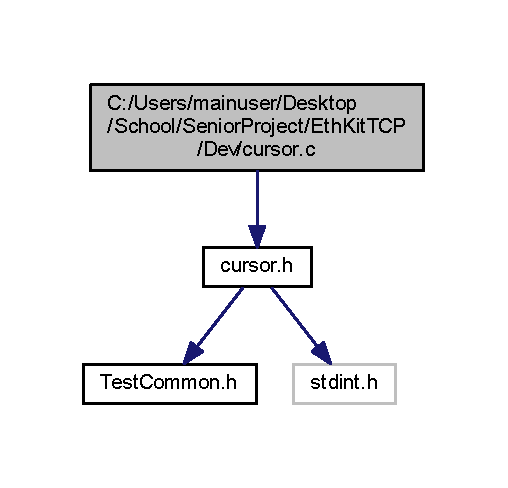
\includegraphics[width=244pt]{cursor_8c__incl}
\end{center}
\end{figure}
\subsection*{Functions}
\begin{DoxyCompactItemize}
\item 
int \hyperlink{cursor_8c_a3a7d62c4f2983e6e2e2f4da56f36befc}{setandget\+Cursor\+Location} (int newcursor\+Location)
\item 
int \hyperlink{cursor_8c_a95873c61ca346ba3ad63577fec99fe15}{get\+Cursor\+Location} (void)
\item 
void \hyperlink{cursor_8c_acd4b06887a4337467e744f693a2df6a9}{set\+Cursor\+Location} (int new\+Cursor\+Location)
\item 
void \hyperlink{cursor_8c_a7804524381705ec22e0efc3a1326dd69}{Move\+Cursor\+Left} (void)
\item 
void \hyperlink{cursor_8c_ac177699cfeda15e4b887864f6eacc5e3}{Move\+Cursor\+Right} (void)
\item 
void \hyperlink{cursor_8c_ae9337ec3c6ea47f10d329cd99d7a29f9}{Move\+Cursor\+Up} (void)
\item 
void \hyperlink{cursor_8c_ac8e40e0b08b773c5f3fc0b303fe562de}{Move\+Cursor\+Down} (void)
\item 
void \hyperlink{cursor_8c_a467458fc0085539f52030fabf3dd9286}{interpret\+\_\+keypress} (char temp)
\item 
void \hyperlink{cursor_8c_aeca62116778bb6c13245089867ded8d9}{reset\+Place\+Char\+Location} (void)
\item 
void \hyperlink{cursor_8c_a9d645a8f1ad2b03ad027accb3bcf0db4}{set\+Text\+Line\+Index} (int newtextlineindex)
\item 
int \hyperlink{cursor_8c_a5c5543d701a9dae494df5b00cc931377}{get\+Text\+Line\+Index} (void)
\item 
void \hyperlink{cursor_8c_aee82caceba560f01202c4459ba4497c7}{process\+Line} (uint8\+\_\+t $\ast$text\+Line\+Ptr)
\item 
void \hyperlink{cursor_8c_a8b0ba534e7681966289c491064e9cdc8}{press\+\_\+\+F1} (void)
\item 
void \hyperlink{cursor_8c_afb368b3eb12755cae8787b96e467e0e3}{press\+\_\+backspace} (void)
\item 
char $\ast$ \hyperlink{cursor_8c_abe73bcf82b19d9727d29850864eac8b8}{get\+I\+P\+Target} ()
\item 
void \hyperlink{cursor_8c_a29bab149333c107091c1b286e05ac315}{place\+Char} (uint8\+\_\+t $\ast$character)
\item 
uint8\+\_\+t $\ast$ \hyperlink{cursor_8c_a3a060fca8f2dde6562e2f243414d47d7}{gettext\+Line} (void)
\item 
void \hyperlink{cursor_8c_a8f55cca82244df1cf78f0a826f816f75}{Compare\+Text\+Lines} (char $\ast$\hyperlink{cursor_8h_a4eddb259269e1401df5b56698f231263}{newtext\+Line})
\item 
void \hyperlink{cursor_8c_a53ebfe2e3649276643adf8647c8a5821}{clear\+Text\+Line} (void)
\item 
void \hyperlink{cursor_8c_a41c92fd026b99457236bf755ee517e55}{add\+Char\+To\+Text\+Line} (char temp2)
\end{DoxyCompactItemize}


\subsection{Function Documentation}
\hypertarget{cursor_8c_a41c92fd026b99457236bf755ee517e55}{}\index{cursor.\+c@{cursor.\+c}!add\+Char\+To\+Text\+Line@{add\+Char\+To\+Text\+Line}}
\index{add\+Char\+To\+Text\+Line@{add\+Char\+To\+Text\+Line}!cursor.\+c@{cursor.\+c}}
\subsubsection[{add\+Char\+To\+Text\+Line}]{\setlength{\rightskip}{0pt plus 5cm}void add\+Char\+To\+Text\+Line (
\begin{DoxyParamCaption}
\item[{char}]{temp2}
\end{DoxyParamCaption}
)}\label{cursor_8c_a41c92fd026b99457236bf755ee517e55}


Definition at line 369 of file cursor.\+c.



Here is the call graph for this function\+:\nopagebreak
\begin{figure}[H]
\begin{center}
\leavevmode
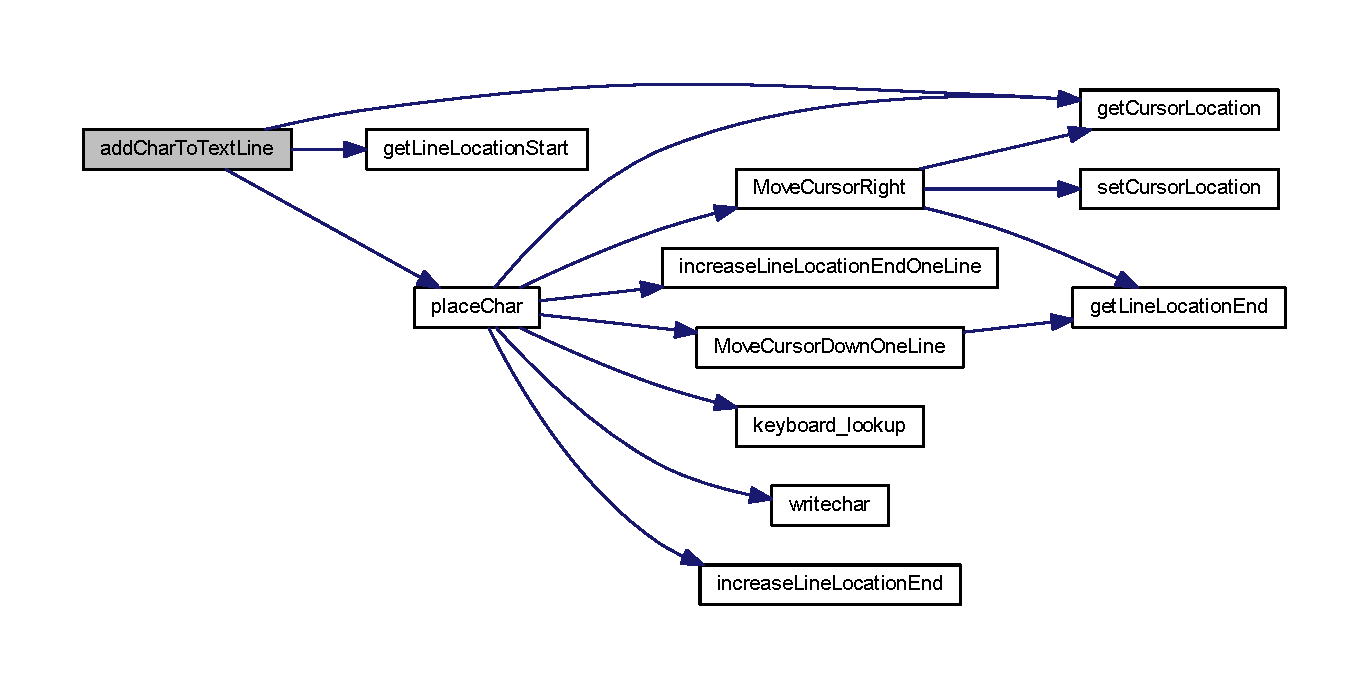
\includegraphics[width=350pt]{cursor_8c_a41c92fd026b99457236bf755ee517e55_cgraph}
\end{center}
\end{figure}




Here is the caller graph for this function\+:\nopagebreak
\begin{figure}[H]
\begin{center}
\leavevmode
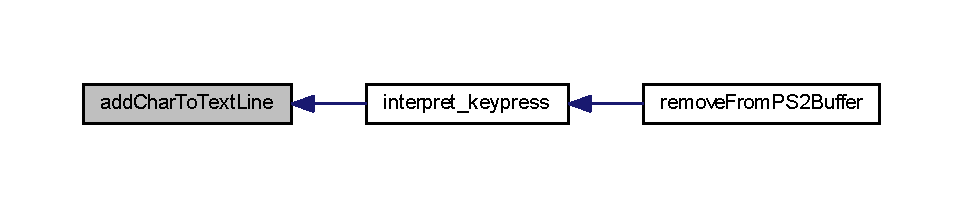
\includegraphics[width=350pt]{cursor_8c_a41c92fd026b99457236bf755ee517e55_icgraph}
\end{center}
\end{figure}


\hypertarget{cursor_8c_a53ebfe2e3649276643adf8647c8a5821}{}\index{cursor.\+c@{cursor.\+c}!clear\+Text\+Line@{clear\+Text\+Line}}
\index{clear\+Text\+Line@{clear\+Text\+Line}!cursor.\+c@{cursor.\+c}}
\subsubsection[{clear\+Text\+Line}]{\setlength{\rightskip}{0pt plus 5cm}void clear\+Text\+Line (
\begin{DoxyParamCaption}
\item[{void}]{}
\end{DoxyParamCaption}
)}\label{cursor_8c_a53ebfe2e3649276643adf8647c8a5821}


Definition at line 360 of file cursor.\+c.



Here is the caller graph for this function\+:\nopagebreak
\begin{figure}[H]
\begin{center}
\leavevmode
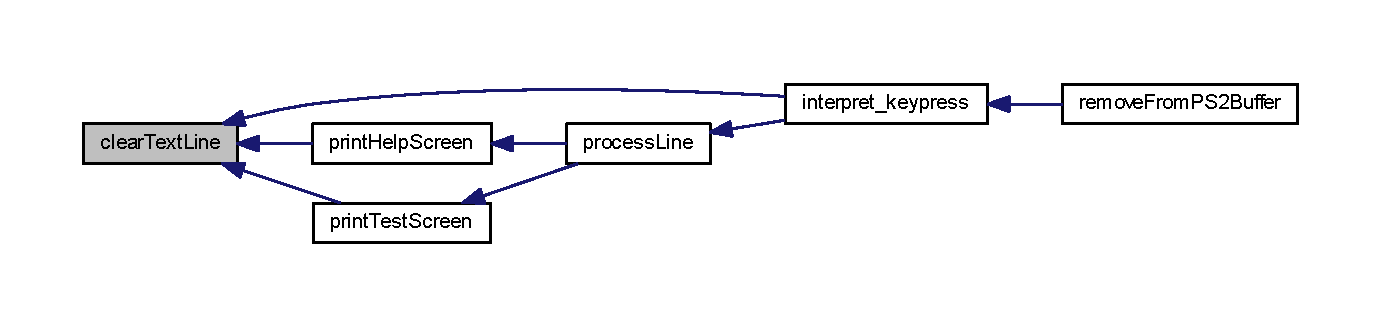
\includegraphics[width=350pt]{cursor_8c_a53ebfe2e3649276643adf8647c8a5821_icgraph}
\end{center}
\end{figure}


\hypertarget{cursor_8c_a8f55cca82244df1cf78f0a826f816f75}{}\index{cursor.\+c@{cursor.\+c}!Compare\+Text\+Lines@{Compare\+Text\+Lines}}
\index{Compare\+Text\+Lines@{Compare\+Text\+Lines}!cursor.\+c@{cursor.\+c}}
\subsubsection[{Compare\+Text\+Lines}]{\setlength{\rightskip}{0pt plus 5cm}void Compare\+Text\+Lines (
\begin{DoxyParamCaption}
\item[{char $\ast$}]{newtext\+Line}
\end{DoxyParamCaption}
)}\label{cursor_8c_a8f55cca82244df1cf78f0a826f816f75}


Definition at line 305 of file cursor.\+c.



Here is the call graph for this function\+:\nopagebreak
\begin{figure}[H]
\begin{center}
\leavevmode
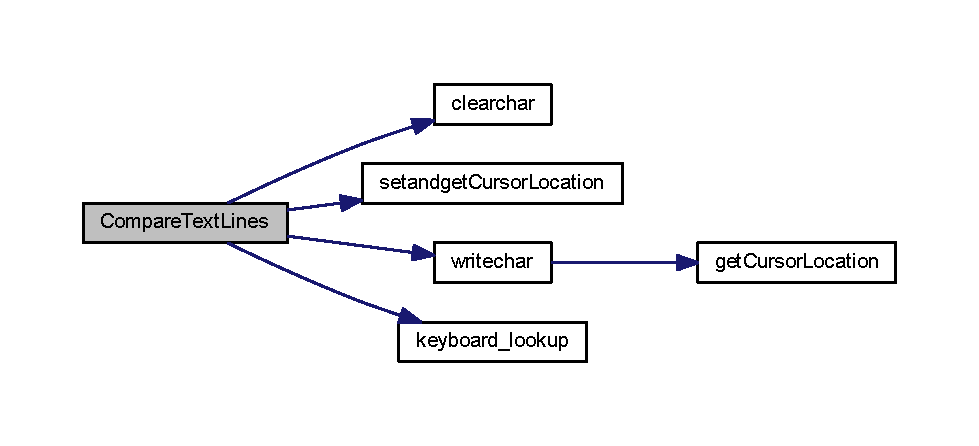
\includegraphics[width=339pt]{cursor_8c_a8f55cca82244df1cf78f0a826f816f75_cgraph}
\end{center}
\end{figure}




Here is the caller graph for this function\+:\nopagebreak
\begin{figure}[H]
\begin{center}
\leavevmode
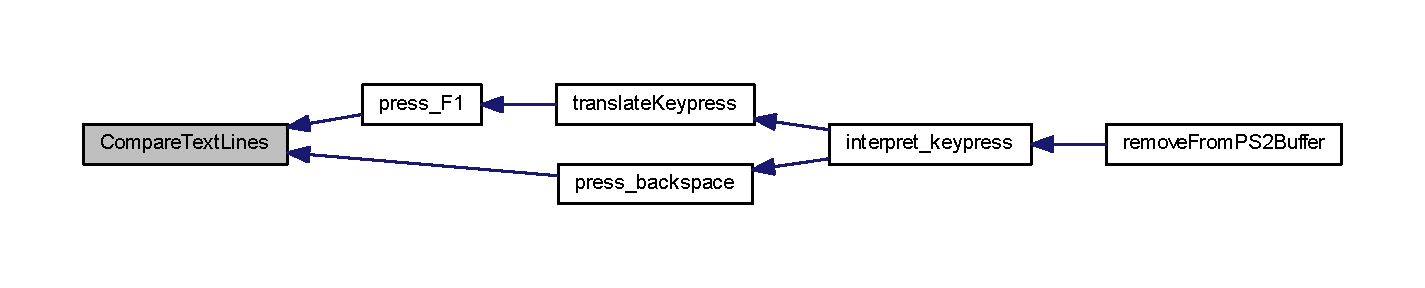
\includegraphics[width=350pt]{cursor_8c_a8f55cca82244df1cf78f0a826f816f75_icgraph}
\end{center}
\end{figure}


\hypertarget{cursor_8c_a95873c61ca346ba3ad63577fec99fe15}{}\index{cursor.\+c@{cursor.\+c}!get\+Cursor\+Location@{get\+Cursor\+Location}}
\index{get\+Cursor\+Location@{get\+Cursor\+Location}!cursor.\+c@{cursor.\+c}}
\subsubsection[{get\+Cursor\+Location}]{\setlength{\rightskip}{0pt plus 5cm}int get\+Cursor\+Location (
\begin{DoxyParamCaption}
\item[{void}]{}
\end{DoxyParamCaption}
)}\label{cursor_8c_a95873c61ca346ba3ad63577fec99fe15}


Definition at line 9 of file cursor.\+c.



Here is the caller graph for this function\+:\nopagebreak
\begin{figure}[H]
\begin{center}
\leavevmode
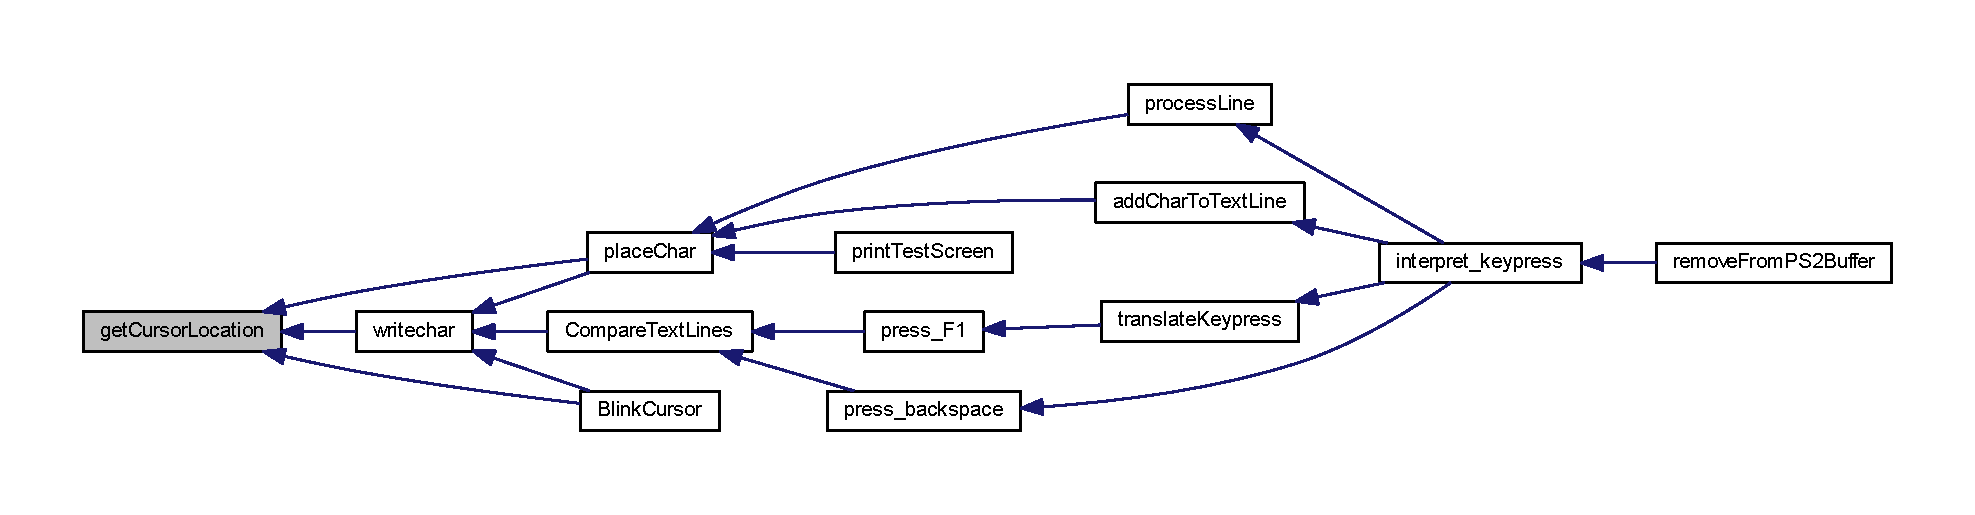
\includegraphics[width=350pt]{cursor_8c_a95873c61ca346ba3ad63577fec99fe15_icgraph}
\end{center}
\end{figure}


\hypertarget{cursor_8c_abe73bcf82b19d9727d29850864eac8b8}{}\index{cursor.\+c@{cursor.\+c}!get\+I\+P\+Target@{get\+I\+P\+Target}}
\index{get\+I\+P\+Target@{get\+I\+P\+Target}!cursor.\+c@{cursor.\+c}}
\subsubsection[{get\+I\+P\+Target}]{\setlength{\rightskip}{0pt plus 5cm}char$\ast$ get\+I\+P\+Target (
\begin{DoxyParamCaption}
{}
\end{DoxyParamCaption}
)}\label{cursor_8c_abe73bcf82b19d9727d29850864eac8b8}


Definition at line 274 of file cursor.\+c.

\hypertarget{cursor_8c_a3a060fca8f2dde6562e2f243414d47d7}{}\index{cursor.\+c@{cursor.\+c}!gettext\+Line@{gettext\+Line}}
\index{gettext\+Line@{gettext\+Line}!cursor.\+c@{cursor.\+c}}
\subsubsection[{gettext\+Line}]{\setlength{\rightskip}{0pt plus 5cm}uint8\+\_\+t$\ast$ gettext\+Line (
\begin{DoxyParamCaption}
\item[{void}]{}
\end{DoxyParamCaption}
)}\label{cursor_8c_a3a060fca8f2dde6562e2f243414d47d7}


Definition at line 297 of file cursor.\+c.

\hypertarget{cursor_8c_a5c5543d701a9dae494df5b00cc931377}{}\index{cursor.\+c@{cursor.\+c}!get\+Text\+Line\+Index@{get\+Text\+Line\+Index}}
\index{get\+Text\+Line\+Index@{get\+Text\+Line\+Index}!cursor.\+c@{cursor.\+c}}
\subsubsection[{get\+Text\+Line\+Index}]{\setlength{\rightskip}{0pt plus 5cm}int get\+Text\+Line\+Index (
\begin{DoxyParamCaption}
\item[{void}]{}
\end{DoxyParamCaption}
)}\label{cursor_8c_a5c5543d701a9dae494df5b00cc931377}


Definition at line 143 of file cursor.\+c.



Here is the caller graph for this function\+:\nopagebreak
\begin{figure}[H]
\begin{center}
\leavevmode
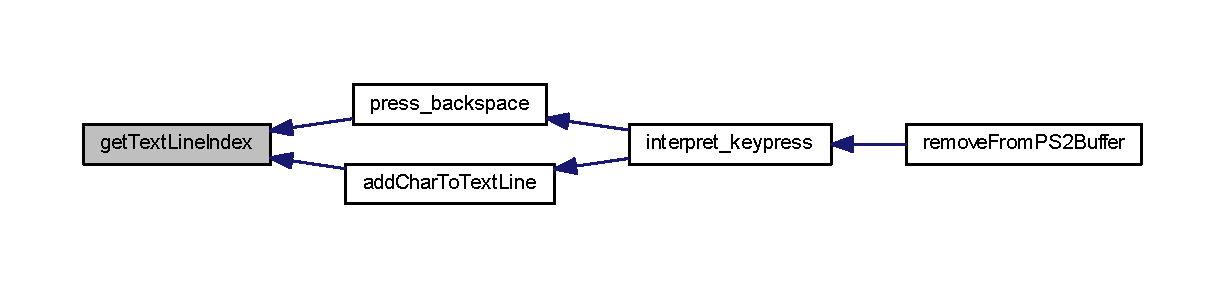
\includegraphics[width=350pt]{cursor_8c_a5c5543d701a9dae494df5b00cc931377_icgraph}
\end{center}
\end{figure}


\hypertarget{cursor_8c_a467458fc0085539f52030fabf3dd9286}{}\index{cursor.\+c@{cursor.\+c}!interpret\+\_\+keypress@{interpret\+\_\+keypress}}
\index{interpret\+\_\+keypress@{interpret\+\_\+keypress}!cursor.\+c@{cursor.\+c}}
\subsubsection[{interpret\+\_\+keypress}]{\setlength{\rightskip}{0pt plus 5cm}void interpret\+\_\+keypress (
\begin{DoxyParamCaption}
\item[{char}]{temp}
\end{DoxyParamCaption}
)}\label{cursor_8c_a467458fc0085539f52030fabf3dd9286}


Definition at line 96 of file cursor.\+c.



Here is the call graph for this function\+:\nopagebreak
\begin{figure}[H]
\begin{center}
\leavevmode
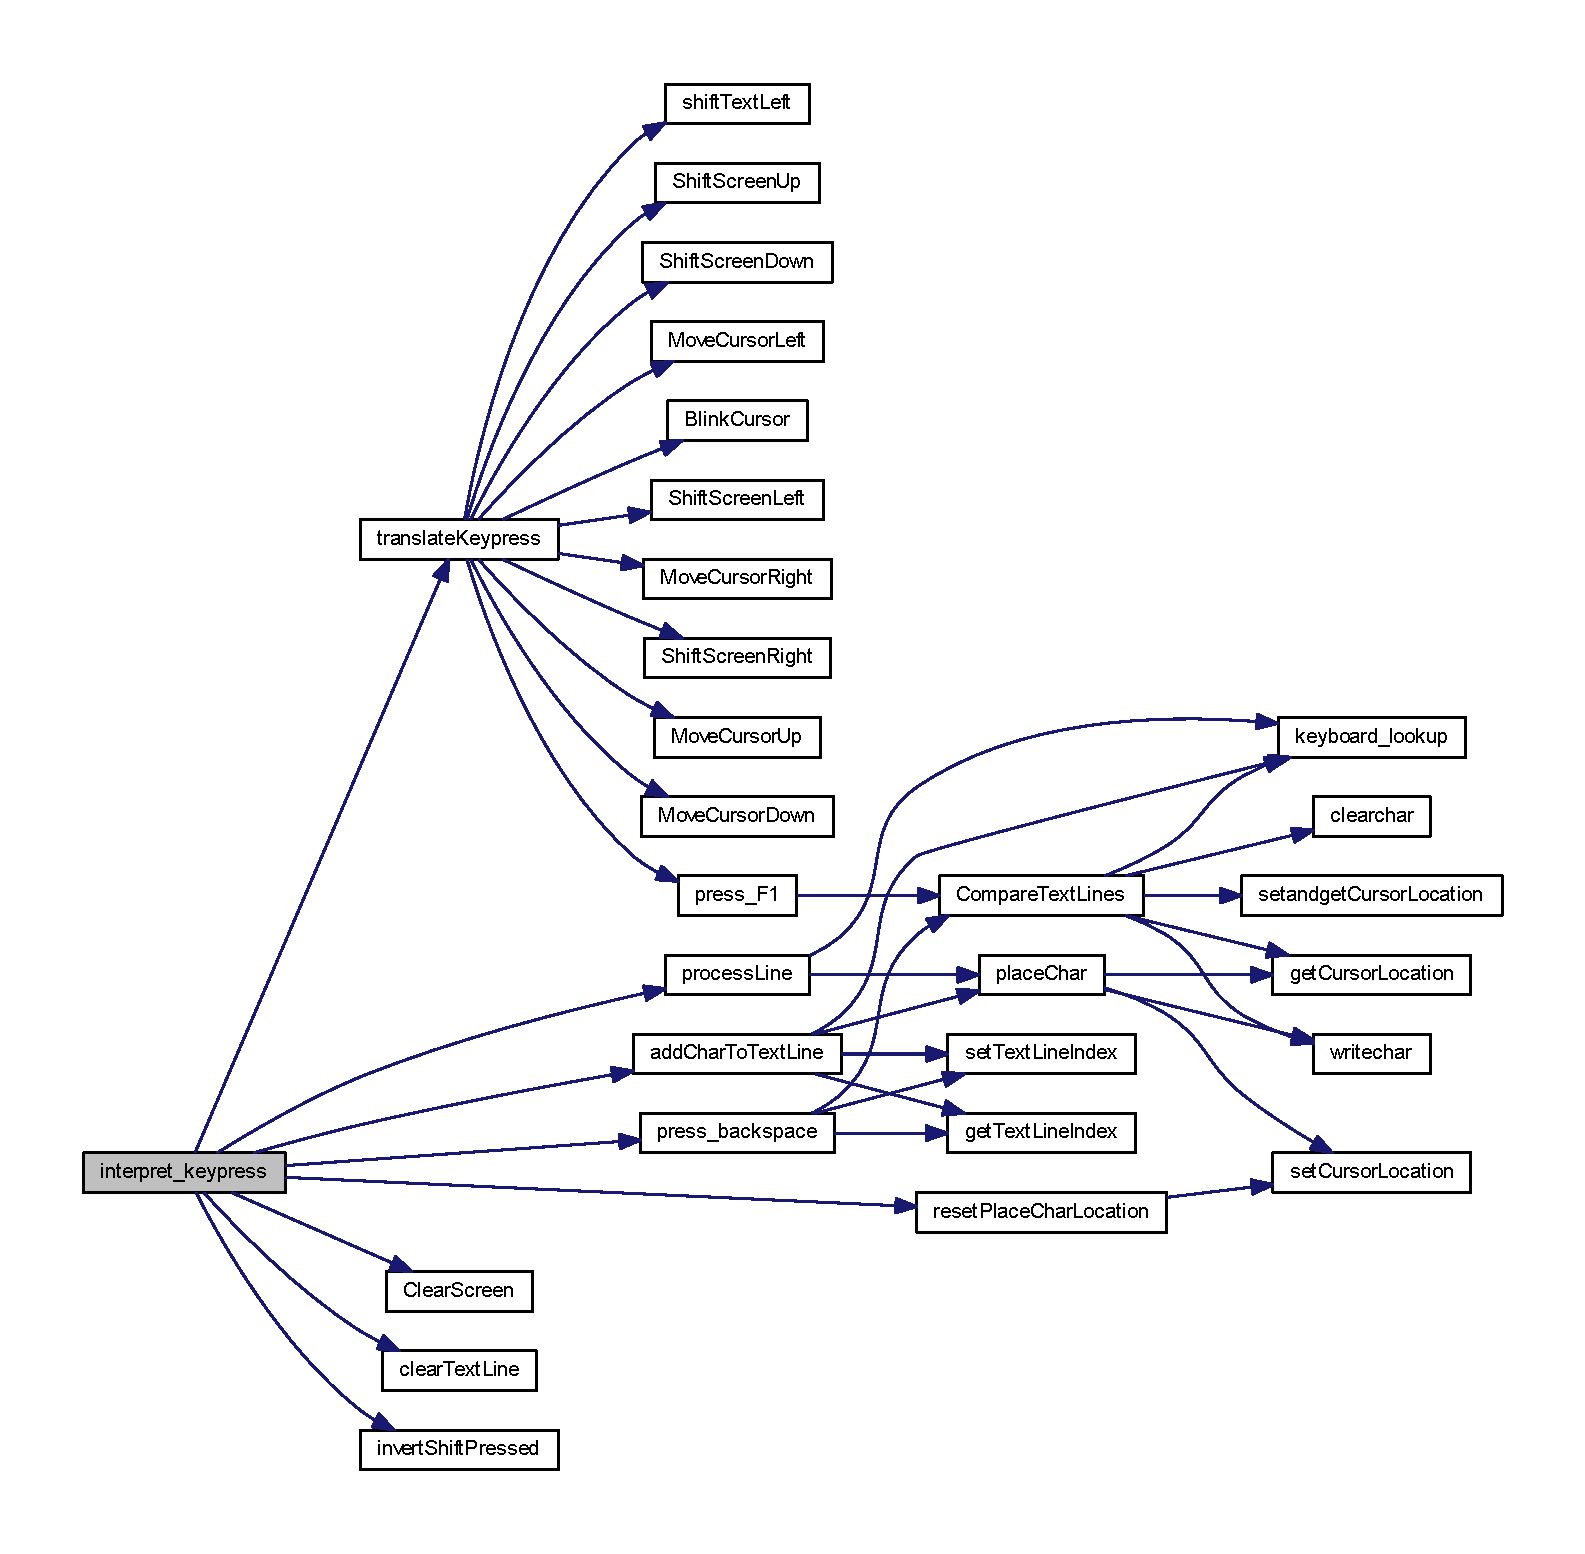
\includegraphics[width=350pt]{cursor_8c_a467458fc0085539f52030fabf3dd9286_cgraph}
\end{center}
\end{figure}




Here is the caller graph for this function\+:\nopagebreak
\begin{figure}[H]
\begin{center}
\leavevmode
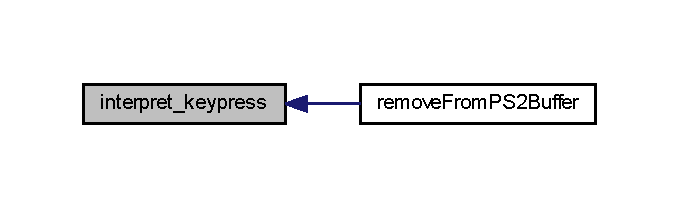
\includegraphics[width=326pt]{cursor_8c_a467458fc0085539f52030fabf3dd9286_icgraph}
\end{center}
\end{figure}


\hypertarget{cursor_8c_ac8e40e0b08b773c5f3fc0b303fe562de}{}\index{cursor.\+c@{cursor.\+c}!Move\+Cursor\+Down@{Move\+Cursor\+Down}}
\index{Move\+Cursor\+Down@{Move\+Cursor\+Down}!cursor.\+c@{cursor.\+c}}
\subsubsection[{Move\+Cursor\+Down}]{\setlength{\rightskip}{0pt plus 5cm}void Move\+Cursor\+Down (
\begin{DoxyParamCaption}
\item[{void}]{}
\end{DoxyParamCaption}
)}\label{cursor_8c_ac8e40e0b08b773c5f3fc0b303fe562de}


Definition at line 72 of file cursor.\+c.



Here is the caller graph for this function\+:\nopagebreak
\begin{figure}[H]
\begin{center}
\leavevmode
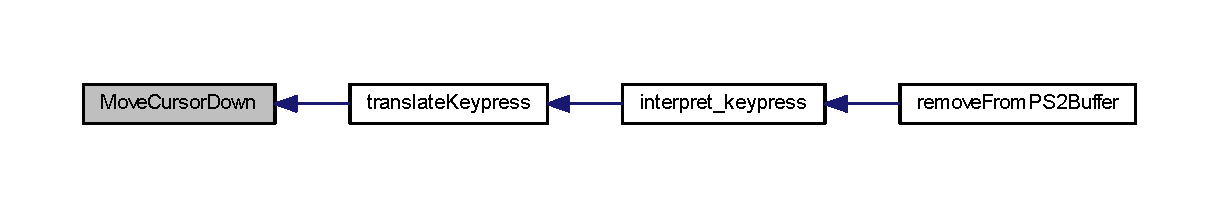
\includegraphics[width=350pt]{cursor_8c_ac8e40e0b08b773c5f3fc0b303fe562de_icgraph}
\end{center}
\end{figure}


\hypertarget{cursor_8c_a7804524381705ec22e0efc3a1326dd69}{}\index{cursor.\+c@{cursor.\+c}!Move\+Cursor\+Left@{Move\+Cursor\+Left}}
\index{Move\+Cursor\+Left@{Move\+Cursor\+Left}!cursor.\+c@{cursor.\+c}}
\subsubsection[{Move\+Cursor\+Left}]{\setlength{\rightskip}{0pt plus 5cm}void Move\+Cursor\+Left (
\begin{DoxyParamCaption}
\item[{void}]{}
\end{DoxyParamCaption}
)}\label{cursor_8c_a7804524381705ec22e0efc3a1326dd69}


Definition at line 19 of file cursor.\+c.



Here is the caller graph for this function\+:\nopagebreak
\begin{figure}[H]
\begin{center}
\leavevmode
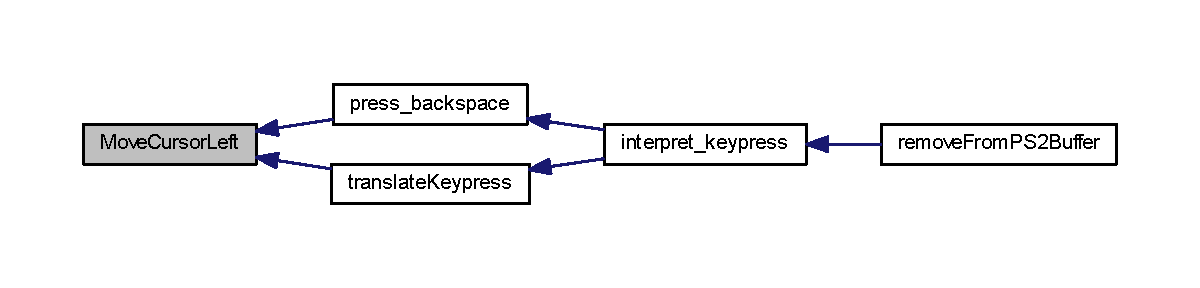
\includegraphics[width=350pt]{cursor_8c_a7804524381705ec22e0efc3a1326dd69_icgraph}
\end{center}
\end{figure}


\hypertarget{cursor_8c_ac177699cfeda15e4b887864f6eacc5e3}{}\index{cursor.\+c@{cursor.\+c}!Move\+Cursor\+Right@{Move\+Cursor\+Right}}
\index{Move\+Cursor\+Right@{Move\+Cursor\+Right}!cursor.\+c@{cursor.\+c}}
\subsubsection[{Move\+Cursor\+Right}]{\setlength{\rightskip}{0pt plus 5cm}void Move\+Cursor\+Right (
\begin{DoxyParamCaption}
\item[{void}]{}
\end{DoxyParamCaption}
)}\label{cursor_8c_ac177699cfeda15e4b887864f6eacc5e3}


Definition at line 40 of file cursor.\+c.



Here is the caller graph for this function\+:\nopagebreak
\begin{figure}[H]
\begin{center}
\leavevmode
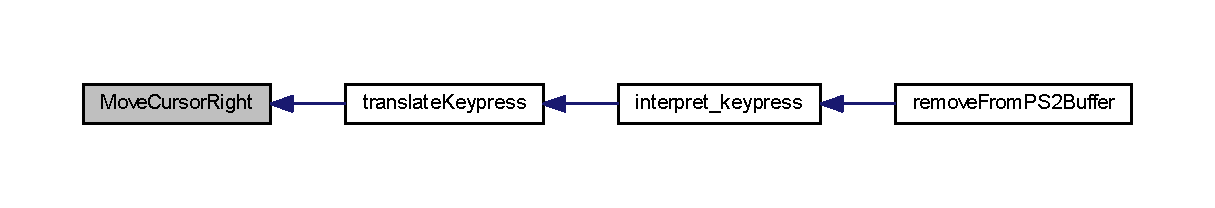
\includegraphics[width=350pt]{cursor_8c_ac177699cfeda15e4b887864f6eacc5e3_icgraph}
\end{center}
\end{figure}


\hypertarget{cursor_8c_ae9337ec3c6ea47f10d329cd99d7a29f9}{}\index{cursor.\+c@{cursor.\+c}!Move\+Cursor\+Up@{Move\+Cursor\+Up}}
\index{Move\+Cursor\+Up@{Move\+Cursor\+Up}!cursor.\+c@{cursor.\+c}}
\subsubsection[{Move\+Cursor\+Up}]{\setlength{\rightskip}{0pt plus 5cm}void Move\+Cursor\+Up (
\begin{DoxyParamCaption}
\item[{void}]{}
\end{DoxyParamCaption}
)}\label{cursor_8c_ae9337ec3c6ea47f10d329cd99d7a29f9}


Definition at line 56 of file cursor.\+c.



Here is the caller graph for this function\+:\nopagebreak
\begin{figure}[H]
\begin{center}
\leavevmode
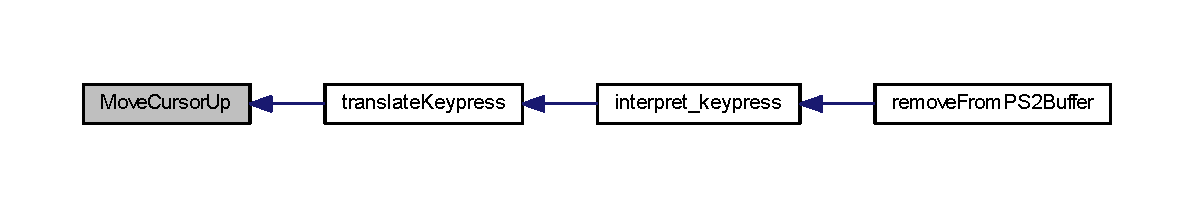
\includegraphics[width=350pt]{cursor_8c_ae9337ec3c6ea47f10d329cd99d7a29f9_icgraph}
\end{center}
\end{figure}


\hypertarget{cursor_8c_a29bab149333c107091c1b286e05ac315}{}\index{cursor.\+c@{cursor.\+c}!place\+Char@{place\+Char}}
\index{place\+Char@{place\+Char}!cursor.\+c@{cursor.\+c}}
\subsubsection[{place\+Char}]{\setlength{\rightskip}{0pt plus 5cm}void place\+Char (
\begin{DoxyParamCaption}
\item[{uint8\+\_\+t $\ast$}]{character}
\end{DoxyParamCaption}
)}\label{cursor_8c_a29bab149333c107091c1b286e05ac315}


Definition at line 279 of file cursor.\+c.



Here is the call graph for this function\+:\nopagebreak
\begin{figure}[H]
\begin{center}
\leavevmode
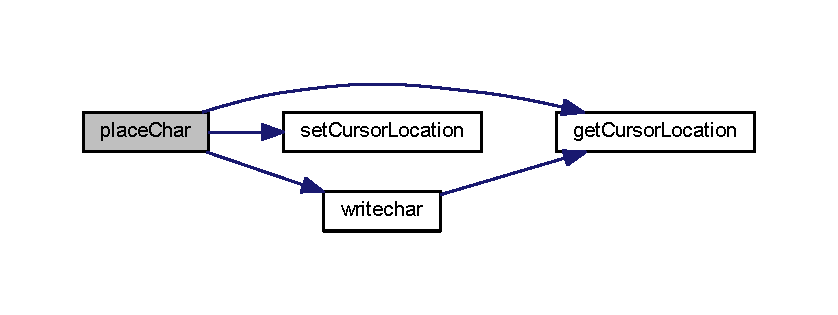
\includegraphics[width=271pt]{cursor_8c_a29bab149333c107091c1b286e05ac315_cgraph}
\end{center}
\end{figure}




Here is the caller graph for this function\+:\nopagebreak
\begin{figure}[H]
\begin{center}
\leavevmode
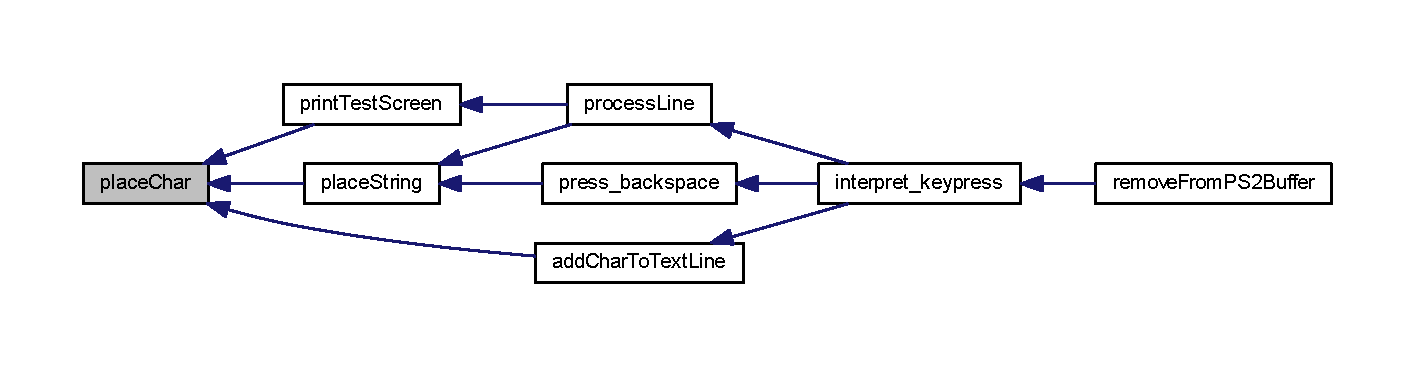
\includegraphics[width=350pt]{cursor_8c_a29bab149333c107091c1b286e05ac315_icgraph}
\end{center}
\end{figure}


\hypertarget{cursor_8c_afb368b3eb12755cae8787b96e467e0e3}{}\index{cursor.\+c@{cursor.\+c}!press\+\_\+backspace@{press\+\_\+backspace}}
\index{press\+\_\+backspace@{press\+\_\+backspace}!cursor.\+c@{cursor.\+c}}
\subsubsection[{press\+\_\+backspace}]{\setlength{\rightskip}{0pt plus 5cm}void press\+\_\+backspace (
\begin{DoxyParamCaption}
\item[{void}]{}
\end{DoxyParamCaption}
)}\label{cursor_8c_afb368b3eb12755cae8787b96e467e0e3}


Definition at line 248 of file cursor.\+c.



Here is the call graph for this function\+:\nopagebreak
\begin{figure}[H]
\begin{center}
\leavevmode
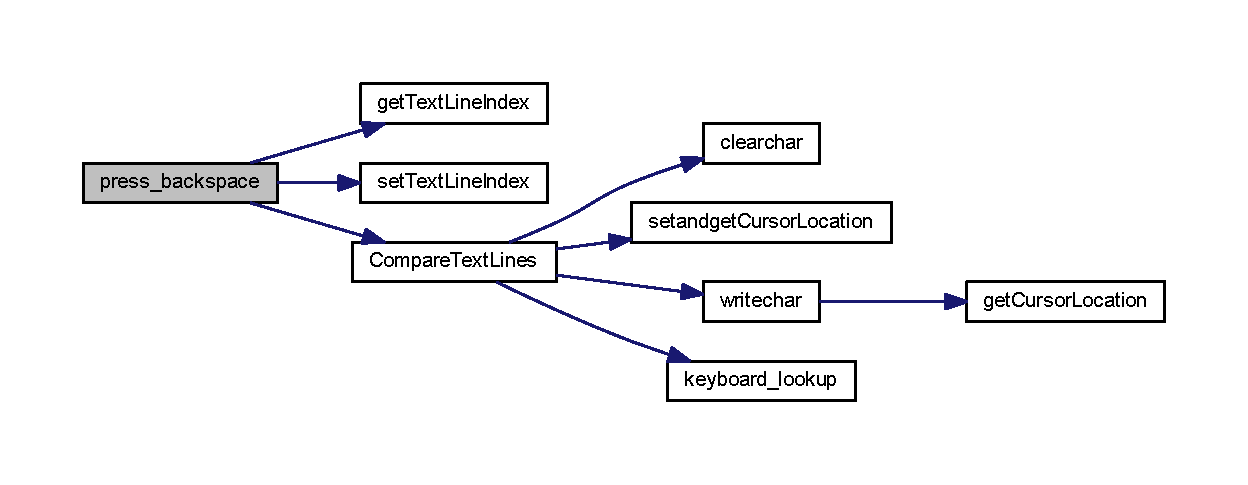
\includegraphics[width=350pt]{cursor_8c_afb368b3eb12755cae8787b96e467e0e3_cgraph}
\end{center}
\end{figure}




Here is the caller graph for this function\+:\nopagebreak
\begin{figure}[H]
\begin{center}
\leavevmode
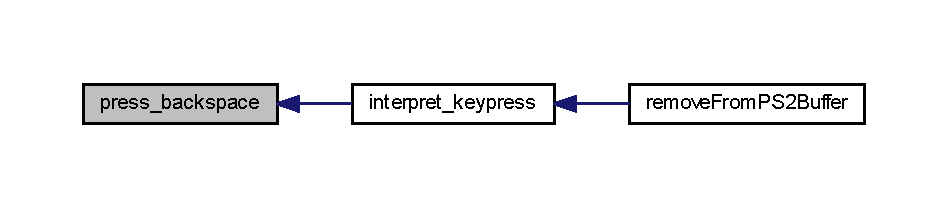
\includegraphics[width=350pt]{cursor_8c_afb368b3eb12755cae8787b96e467e0e3_icgraph}
\end{center}
\end{figure}


\hypertarget{cursor_8c_a8b0ba534e7681966289c491064e9cdc8}{}\index{cursor.\+c@{cursor.\+c}!press\+\_\+\+F1@{press\+\_\+\+F1}}
\index{press\+\_\+\+F1@{press\+\_\+\+F1}!cursor.\+c@{cursor.\+c}}
\subsubsection[{press\+\_\+\+F1}]{\setlength{\rightskip}{0pt plus 5cm}void press\+\_\+\+F1 (
\begin{DoxyParamCaption}
\item[{void}]{}
\end{DoxyParamCaption}
)}\label{cursor_8c_a8b0ba534e7681966289c491064e9cdc8}


Definition at line 234 of file cursor.\+c.



Here is the call graph for this function\+:\nopagebreak
\begin{figure}[H]
\begin{center}
\leavevmode
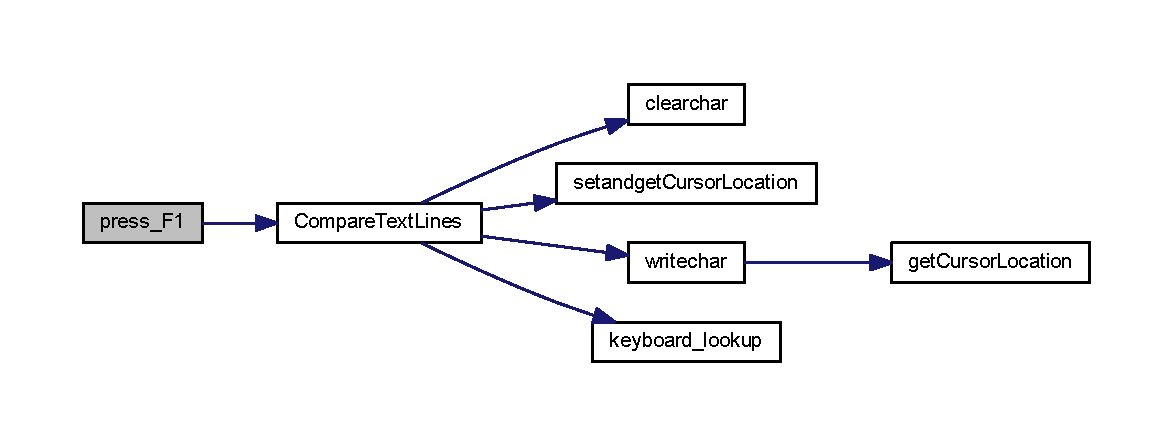
\includegraphics[width=350pt]{cursor_8c_a8b0ba534e7681966289c491064e9cdc8_cgraph}
\end{center}
\end{figure}




Here is the caller graph for this function\+:\nopagebreak
\begin{figure}[H]
\begin{center}
\leavevmode
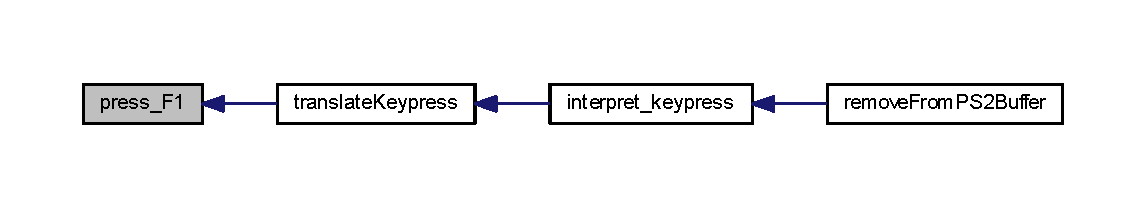
\includegraphics[width=350pt]{cursor_8c_a8b0ba534e7681966289c491064e9cdc8_icgraph}
\end{center}
\end{figure}


\hypertarget{cursor_8c_aee82caceba560f01202c4459ba4497c7}{}\index{cursor.\+c@{cursor.\+c}!process\+Line@{process\+Line}}
\index{process\+Line@{process\+Line}!cursor.\+c@{cursor.\+c}}
\subsubsection[{process\+Line}]{\setlength{\rightskip}{0pt plus 5cm}void process\+Line (
\begin{DoxyParamCaption}
\item[{uint8\+\_\+t $\ast$}]{text\+Line\+Ptr}
\end{DoxyParamCaption}
)}\label{cursor_8c_aee82caceba560f01202c4459ba4497c7}


Definition at line 149 of file cursor.\+c.



Here is the call graph for this function\+:\nopagebreak
\begin{figure}[H]
\begin{center}
\leavevmode
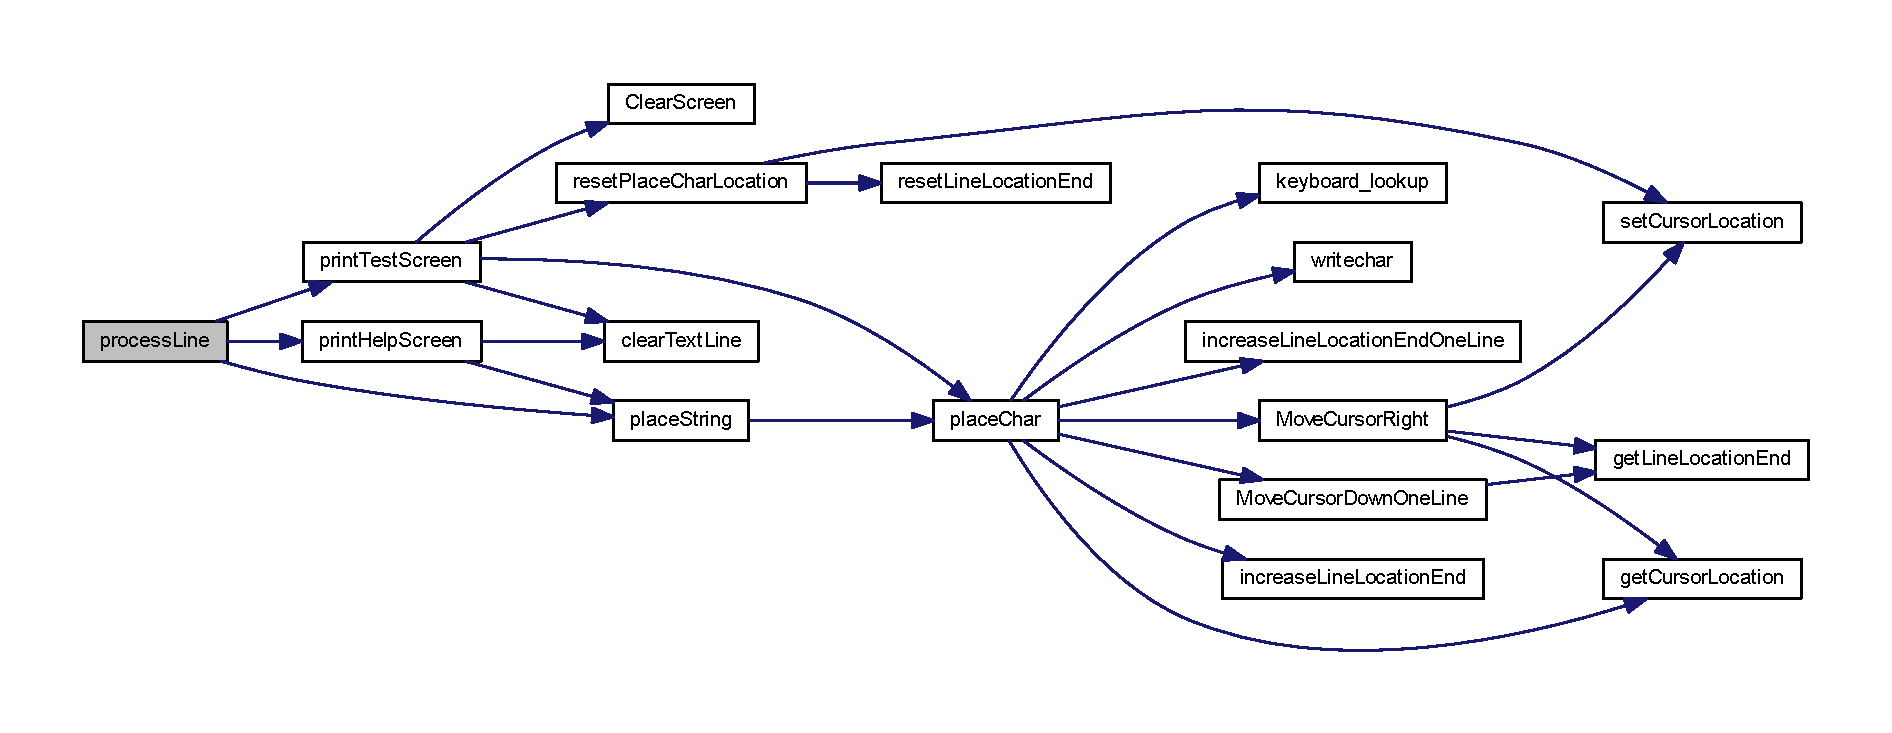
\includegraphics[width=350pt]{cursor_8c_aee82caceba560f01202c4459ba4497c7_cgraph}
\end{center}
\end{figure}




Here is the caller graph for this function\+:\nopagebreak
\begin{figure}[H]
\begin{center}
\leavevmode
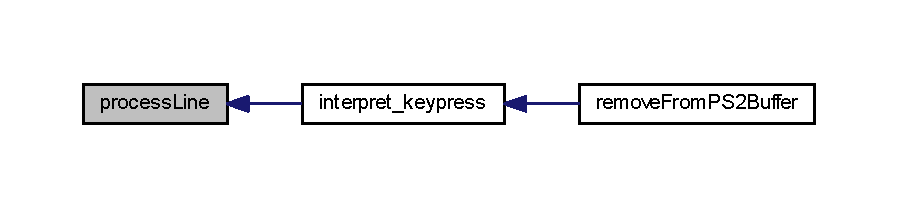
\includegraphics[width=350pt]{cursor_8c_aee82caceba560f01202c4459ba4497c7_icgraph}
\end{center}
\end{figure}


\hypertarget{cursor_8c_aeca62116778bb6c13245089867ded8d9}{}\index{cursor.\+c@{cursor.\+c}!reset\+Place\+Char\+Location@{reset\+Place\+Char\+Location}}
\index{reset\+Place\+Char\+Location@{reset\+Place\+Char\+Location}!cursor.\+c@{cursor.\+c}}
\subsubsection[{reset\+Place\+Char\+Location}]{\setlength{\rightskip}{0pt plus 5cm}void reset\+Place\+Char\+Location (
\begin{DoxyParamCaption}
\item[{void}]{}
\end{DoxyParamCaption}
)}\label{cursor_8c_aeca62116778bb6c13245089867ded8d9}


Definition at line 132 of file cursor.\+c.



Here is the call graph for this function\+:\nopagebreak
\begin{figure}[H]
\begin{center}
\leavevmode
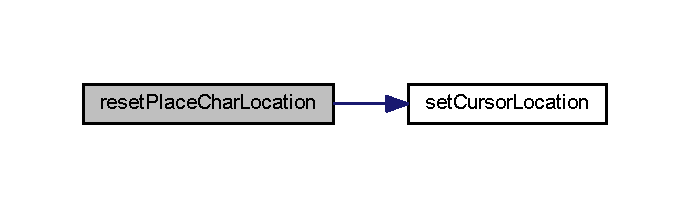
\includegraphics[width=331pt]{cursor_8c_aeca62116778bb6c13245089867ded8d9_cgraph}
\end{center}
\end{figure}




Here is the caller graph for this function\+:\nopagebreak
\begin{figure}[H]
\begin{center}
\leavevmode
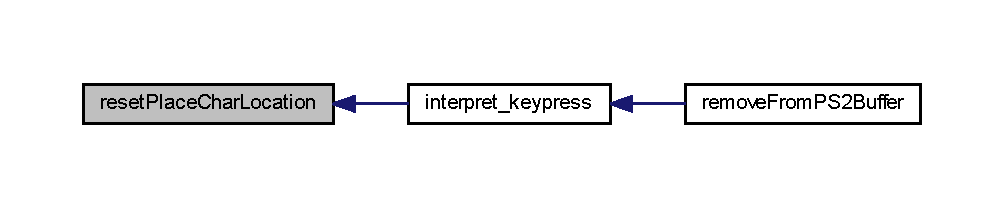
\includegraphics[width=350pt]{cursor_8c_aeca62116778bb6c13245089867ded8d9_icgraph}
\end{center}
\end{figure}


\hypertarget{cursor_8c_a3a7d62c4f2983e6e2e2f4da56f36befc}{}\index{cursor.\+c@{cursor.\+c}!setandget\+Cursor\+Location@{setandget\+Cursor\+Location}}
\index{setandget\+Cursor\+Location@{setandget\+Cursor\+Location}!cursor.\+c@{cursor.\+c}}
\subsubsection[{setandget\+Cursor\+Location}]{\setlength{\rightskip}{0pt plus 5cm}int setandget\+Cursor\+Location (
\begin{DoxyParamCaption}
\item[{int}]{newcursor\+Location}
\end{DoxyParamCaption}
)}\label{cursor_8c_a3a7d62c4f2983e6e2e2f4da56f36befc}


Definition at line 3 of file cursor.\+c.



Here is the caller graph for this function\+:\nopagebreak
\begin{figure}[H]
\begin{center}
\leavevmode
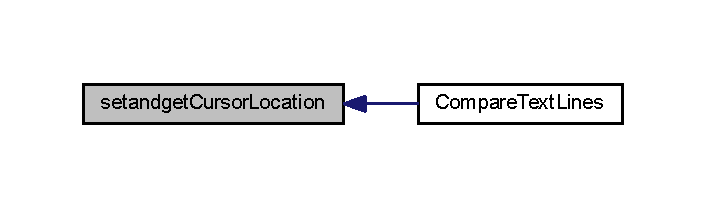
\includegraphics[width=350pt]{cursor_8c_a3a7d62c4f2983e6e2e2f4da56f36befc_icgraph}
\end{center}
\end{figure}


\hypertarget{cursor_8c_acd4b06887a4337467e744f693a2df6a9}{}\index{cursor.\+c@{cursor.\+c}!set\+Cursor\+Location@{set\+Cursor\+Location}}
\index{set\+Cursor\+Location@{set\+Cursor\+Location}!cursor.\+c@{cursor.\+c}}
\subsubsection[{set\+Cursor\+Location}]{\setlength{\rightskip}{0pt plus 5cm}void set\+Cursor\+Location (
\begin{DoxyParamCaption}
\item[{int}]{new\+Cursor\+Location}
\end{DoxyParamCaption}
)}\label{cursor_8c_acd4b06887a4337467e744f693a2df6a9}


Definition at line 14 of file cursor.\+c.



Here is the caller graph for this function\+:\nopagebreak
\begin{figure}[H]
\begin{center}
\leavevmode
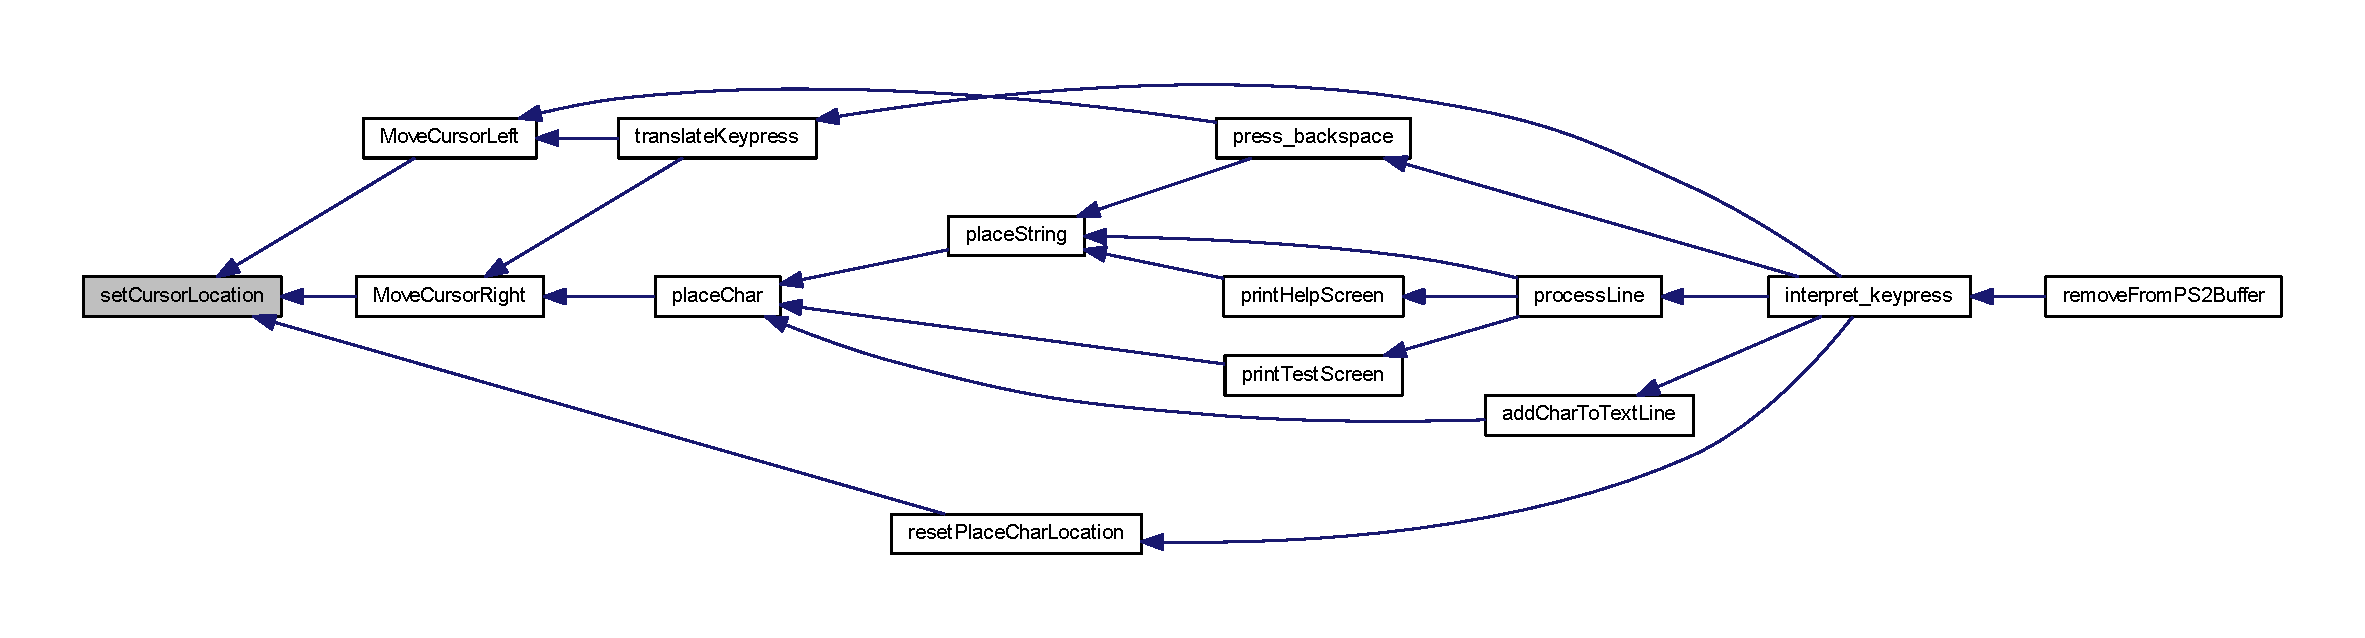
\includegraphics[width=350pt]{cursor_8c_acd4b06887a4337467e744f693a2df6a9_icgraph}
\end{center}
\end{figure}


\hypertarget{cursor_8c_a9d645a8f1ad2b03ad027accb3bcf0db4}{}\index{cursor.\+c@{cursor.\+c}!set\+Text\+Line\+Index@{set\+Text\+Line\+Index}}
\index{set\+Text\+Line\+Index@{set\+Text\+Line\+Index}!cursor.\+c@{cursor.\+c}}
\subsubsection[{set\+Text\+Line\+Index}]{\setlength{\rightskip}{0pt plus 5cm}void set\+Text\+Line\+Index (
\begin{DoxyParamCaption}
\item[{int}]{newtextlineindex}
\end{DoxyParamCaption}
)}\label{cursor_8c_a9d645a8f1ad2b03ad027accb3bcf0db4}


Definition at line 138 of file cursor.\+c.



Here is the caller graph for this function\+:\nopagebreak
\begin{figure}[H]
\begin{center}
\leavevmode
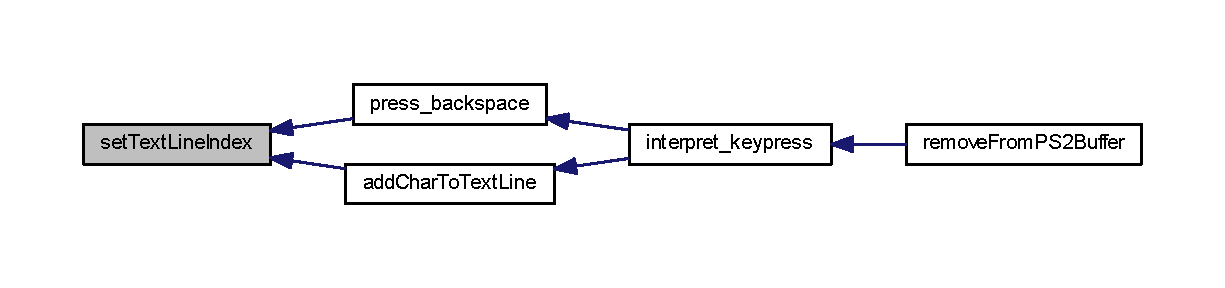
\includegraphics[width=350pt]{cursor_8c_a9d645a8f1ad2b03ad027accb3bcf0db4_icgraph}
\end{center}
\end{figure}



\hypertarget{cursor_8h}{}\section{D\+:/\+School/\+Senior\+Project/\+Eth\+Kit\+T\+C\+P/\+Dev/cursor.h File Reference}
\label{cursor_8h}\index{D\+:/\+School/\+Senior\+Project/\+Eth\+Kit\+T\+C\+P/\+Dev/cursor.\+h@{D\+:/\+School/\+Senior\+Project/\+Eth\+Kit\+T\+C\+P/\+Dev/cursor.\+h}}
{\ttfamily \#include \char`\"{}Test\+Common.\+h\char`\"{}}\\*
{\ttfamily \#include $<$stdint.\+h$>$}\\*
Include dependency graph for cursor.\+h\+:\nopagebreak
\begin{figure}[H]
\begin{center}
\leavevmode
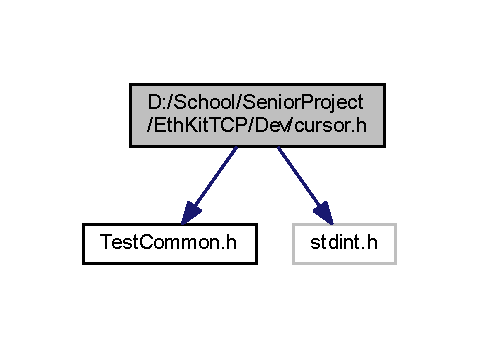
\includegraphics[width=230pt]{cursor_8h__incl}
\end{center}
\end{figure}
This graph shows which files directly or indirectly include this file\+:\nopagebreak
\begin{figure}[H]
\begin{center}
\leavevmode
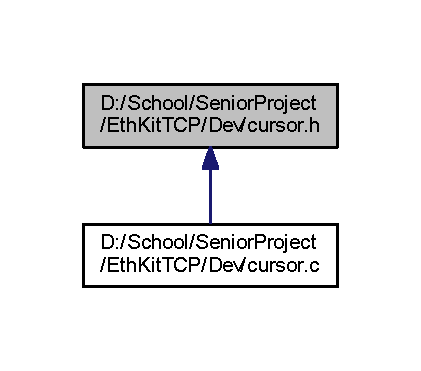
\includegraphics[width=202pt]{cursor_8h__dep__incl}
\end{center}
\end{figure}
\subsection*{Macros}
\begin{DoxyCompactItemize}
\item 
\#define \hyperlink{cursor_8h_a01882b20b26727e0c233e94a4c863459}{T\+E\+X\+T\+L\+I\+N\+E\+L\+E\+N\+G\+T\+H}~7500
\end{DoxyCompactItemize}
\subsection*{Functions}
\begin{DoxyCompactItemize}
\item 
int \hyperlink{cursor_8h_a3a7d62c4f2983e6e2e2f4da56f36befc}{setandget\+Cursor\+Location} (int newcursor\+Location)
\item 
int \hyperlink{cursor_8h_a5a986a90cba784aeb2039295362a6282}{get\+Cursor\+Location} ()
\item 
void \hyperlink{cursor_8h_acd4b06887a4337467e744f693a2df6a9}{set\+Cursor\+Location} (int new\+Cursor\+Location)
\item 
void \hyperlink{cursor_8h_a06559067271121a8ba77c7e7f387a8f3}{increase\+Line\+Location\+End} (void)
\item 
void \hyperlink{cursor_8h_ad74454a9d14ccfe37bfa622791fa47e8}{increase\+Line\+Location\+End\+One\+Line} (void)
\item 
void \hyperlink{cursor_8h_aa510ca0bb56c03148f3392c28433dc45}{decrease\+Line\+Location\+End} (void)
\item 
int \hyperlink{cursor_8h_a52e93559a57ee99d14ce6d275cbb47a6}{get\+Line\+Location\+Start} (void)
\item 
void \hyperlink{cursor_8h_a453e2db022d7de17533e1509906065c9}{set\+Line\+Location\+Start} (int new\+Line\+Location\+Start)
\item 
void \hyperlink{cursor_8h_a7804524381705ec22e0efc3a1326dd69}{Move\+Cursor\+Left} (void)
\item 
void \hyperlink{cursor_8h_ac177699cfeda15e4b887864f6eacc5e3}{Move\+Cursor\+Right} (void)
\item 
void \hyperlink{cursor_8h_ae9337ec3c6ea47f10d329cd99d7a29f9}{Move\+Cursor\+Up} (void)
\item 
void \hyperlink{cursor_8h_ac8e40e0b08b773c5f3fc0b303fe562de}{Move\+Cursor\+Down} (void)
\item 
void \hyperlink{cursor_8h_aa0d5d4e3acd447e87fdab37d7388df23}{Move\+Cursor\+Down\+One\+Line} (void)
\item 
void \hyperlink{cursor_8h_a467458fc0085539f52030fabf3dd9286}{interpret\+\_\+keypress} (char temp)
\item 
void \hyperlink{cursor_8h_aeca62116778bb6c13245089867ded8d9}{reset\+Place\+Char\+Location} (void)
\item 
void \hyperlink{cursor_8h_aee82caceba560f01202c4459ba4497c7}{process\+Line} (uint8\+\_\+t $\ast$text\+Line\+Ptr)
\item 
void \hyperlink{cursor_8h_afb368b3eb12755cae8787b96e467e0e3}{press\+\_\+backspace} (void)
\item 
char $\ast$ \hyperlink{cursor_8h_abe73bcf82b19d9727d29850864eac8b8}{get\+I\+P\+Target} ()
\item 
void \hyperlink{cursor_8h_a8d48f16d45338842dc6cbb3256eb7dae}{place\+Char} (uint8\+\_\+t character)
\item 
void \hyperlink{cursor_8h_a02936826fc9c1380ef1e42ae18940c9a}{place\+String} (char $\ast$string)
\item 
uint8\+\_\+t $\ast$ \hyperlink{cursor_8h_a3a060fca8f2dde6562e2f243414d47d7}{gettext\+Line} (void)
\item 
void \hyperlink{cursor_8h_a8f55cca82244df1cf78f0a826f816f75}{Compare\+Text\+Lines} (char $\ast$\hyperlink{cursor_8h_a4eddb259269e1401df5b56698f231263}{newtext\+Line})
\item 
void \hyperlink{cursor_8h_aa68556b6a4e7315e031e8f18361d283e}{print\+Help\+Screen} (void)
\item 
void \hyperlink{cursor_8h_ab66a8865de62d9daefab9f8abf026478}{print\+Test\+Screen} (void)
\end{DoxyCompactItemize}
\subsection*{Variables}
\begin{DoxyCompactItemize}
\item 
int \hyperlink{cursor_8h_a06590bd84e8fca8ad5292a6e5ca50890}{Cursor\+Location}
\item 
int \hyperlink{cursor_8h_a96a71abb37405cb6ad878a4adac6d177}{Line\+Location\+Start}
\item 
int \hyperlink{cursor_8h_a9edd5050c7ee33f44c008e98933880e0}{Line\+Location\+End}
\item 
char \hyperlink{cursor_8h_aa4e0d20faf2f41acbf49d137715ba813}{I\+P\+Target} \mbox{[}16\mbox{]}
\item 
uint8\+\_\+t \hyperlink{cursor_8h_a78a502c5ea8364e4c06aea5ff4361c8f}{text\+Line} \mbox{[}\hyperlink{cursor_8h_a01882b20b26727e0c233e94a4c863459}{T\+E\+X\+T\+L\+I\+N\+E\+L\+E\+N\+G\+T\+H}\mbox{]}
\item 
uint8\+\_\+t \hyperlink{cursor_8h_a4eddb259269e1401df5b56698f231263}{newtext\+Line} \mbox{[}\hyperlink{cursor_8h_a01882b20b26727e0c233e94a4c863459}{T\+E\+X\+T\+L\+I\+N\+E\+L\+E\+N\+G\+T\+H}\mbox{]}
\end{DoxyCompactItemize}


\subsection{Macro Definition Documentation}
\hypertarget{cursor_8h_a01882b20b26727e0c233e94a4c863459}{}\index{cursor.\+h@{cursor.\+h}!T\+E\+X\+T\+L\+I\+N\+E\+L\+E\+N\+G\+T\+H@{T\+E\+X\+T\+L\+I\+N\+E\+L\+E\+N\+G\+T\+H}}
\index{T\+E\+X\+T\+L\+I\+N\+E\+L\+E\+N\+G\+T\+H@{T\+E\+X\+T\+L\+I\+N\+E\+L\+E\+N\+G\+T\+H}!cursor.\+h@{cursor.\+h}}
\subsubsection[{T\+E\+X\+T\+L\+I\+N\+E\+L\+E\+N\+G\+T\+H}]{\setlength{\rightskip}{0pt plus 5cm}\#define T\+E\+X\+T\+L\+I\+N\+E\+L\+E\+N\+G\+T\+H~7500}\label{cursor_8h_a01882b20b26727e0c233e94a4c863459}


Definition at line 76 of file cursor.\+h.



\subsection{Function Documentation}
\hypertarget{cursor_8h_a8f55cca82244df1cf78f0a826f816f75}{}\index{cursor.\+h@{cursor.\+h}!Compare\+Text\+Lines@{Compare\+Text\+Lines}}
\index{Compare\+Text\+Lines@{Compare\+Text\+Lines}!cursor.\+h@{cursor.\+h}}
\subsubsection[{Compare\+Text\+Lines}]{\setlength{\rightskip}{0pt plus 5cm}void Compare\+Text\+Lines (
\begin{DoxyParamCaption}
\item[{char $\ast$}]{newtext\+Line}
\end{DoxyParamCaption}
)}\label{cursor_8h_a8f55cca82244df1cf78f0a826f816f75}


Definition at line 514 of file cursor.\+c.



Here is the call graph for this function\+:\nopagebreak
\begin{figure}[H]
\begin{center}
\leavevmode
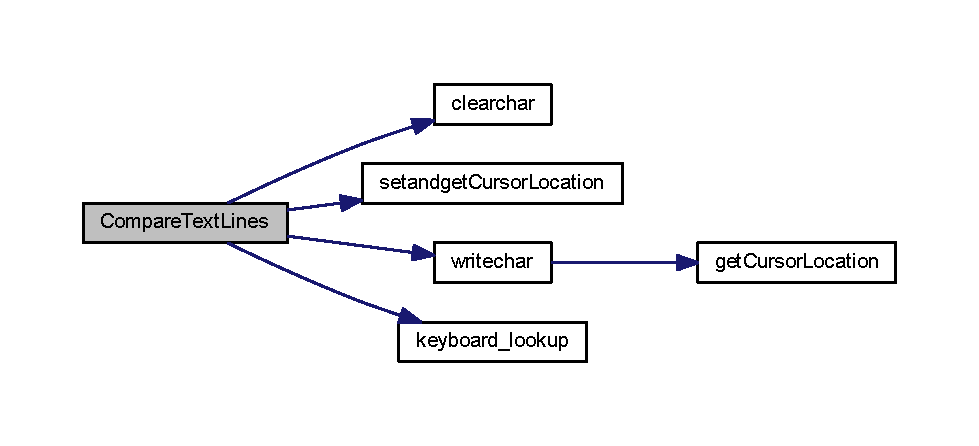
\includegraphics[width=339pt]{cursor_8h_a8f55cca82244df1cf78f0a826f816f75_cgraph}
\end{center}
\end{figure}




Here is the caller graph for this function\+:\nopagebreak
\begin{figure}[H]
\begin{center}
\leavevmode
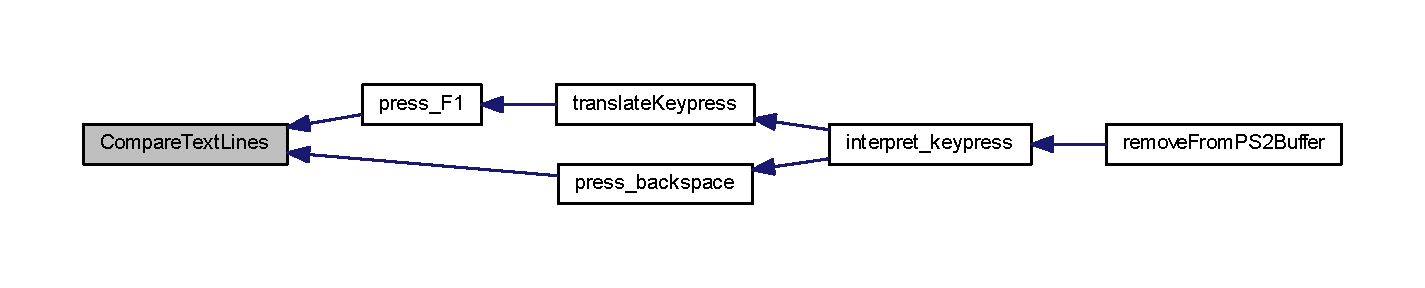
\includegraphics[width=350pt]{cursor_8h_a8f55cca82244df1cf78f0a826f816f75_icgraph}
\end{center}
\end{figure}


\hypertarget{cursor_8h_aa510ca0bb56c03148f3392c28433dc45}{}\index{cursor.\+h@{cursor.\+h}!decrease\+Line\+Location\+End@{decrease\+Line\+Location\+End}}
\index{decrease\+Line\+Location\+End@{decrease\+Line\+Location\+End}!cursor.\+h@{cursor.\+h}}
\subsubsection[{decrease\+Line\+Location\+End}]{\setlength{\rightskip}{0pt plus 5cm}void decrease\+Line\+Location\+End (
\begin{DoxyParamCaption}
\item[{void}]{}
\end{DoxyParamCaption}
)}\label{cursor_8h_aa510ca0bb56c03148f3392c28433dc45}


Definition at line 129 of file cursor.\+c.



Here is the caller graph for this function\+:\nopagebreak
\begin{figure}[H]
\begin{center}
\leavevmode
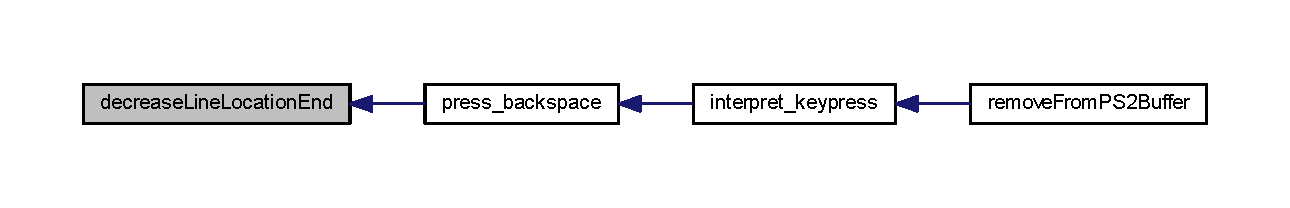
\includegraphics[width=350pt]{cursor_8h_aa510ca0bb56c03148f3392c28433dc45_icgraph}
\end{center}
\end{figure}


\hypertarget{cursor_8h_a5a986a90cba784aeb2039295362a6282}{}\index{cursor.\+h@{cursor.\+h}!get\+Cursor\+Location@{get\+Cursor\+Location}}
\index{get\+Cursor\+Location@{get\+Cursor\+Location}!cursor.\+h@{cursor.\+h}}
\subsubsection[{get\+Cursor\+Location}]{\setlength{\rightskip}{0pt plus 5cm}int get\+Cursor\+Location (
\begin{DoxyParamCaption}
\item[{void}]{}
\end{DoxyParamCaption}
)}\label{cursor_8h_a5a986a90cba784aeb2039295362a6282}
Gets the cursor location \begin{DoxyReturn}{Returns}
Cursor\+Location 
\end{DoxyReturn}


Definition at line 16 of file cursor.\+c.



Here is the caller graph for this function\+:\nopagebreak
\begin{figure}[H]
\begin{center}
\leavevmode
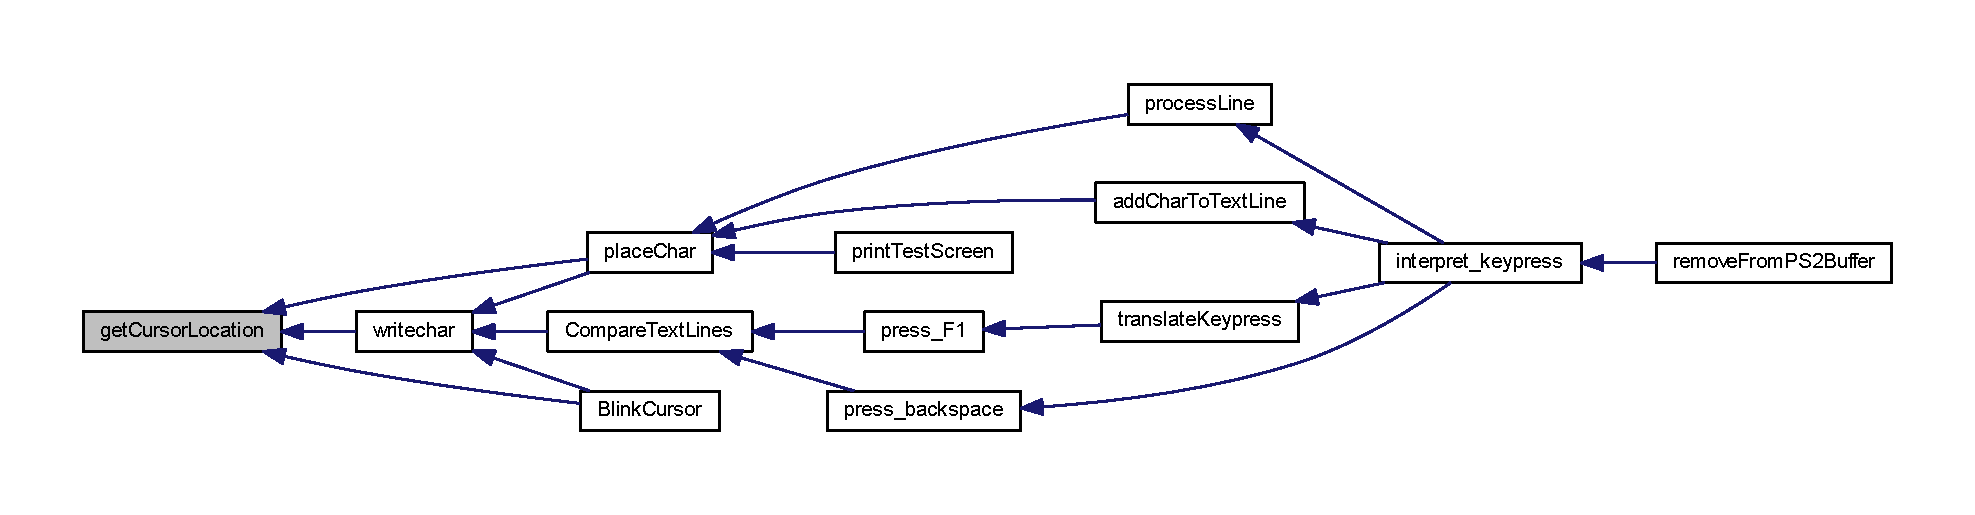
\includegraphics[width=350pt]{cursor_8h_a5a986a90cba784aeb2039295362a6282_icgraph}
\end{center}
\end{figure}


\hypertarget{cursor_8h_abe73bcf82b19d9727d29850864eac8b8}{}\index{cursor.\+h@{cursor.\+h}!get\+I\+P\+Target@{get\+I\+P\+Target}}
\index{get\+I\+P\+Target@{get\+I\+P\+Target}!cursor.\+h@{cursor.\+h}}
\subsubsection[{get\+I\+P\+Target}]{\setlength{\rightskip}{0pt plus 5cm}char$\ast$ get\+I\+P\+Target (
\begin{DoxyParamCaption}
{}
\end{DoxyParamCaption}
)}\label{cursor_8h_abe73bcf82b19d9727d29850864eac8b8}


Definition at line 435 of file cursor.\+c.

\hypertarget{cursor_8h_a52e93559a57ee99d14ce6d275cbb47a6}{}\index{cursor.\+h@{cursor.\+h}!get\+Line\+Location\+Start@{get\+Line\+Location\+Start}}
\index{get\+Line\+Location\+Start@{get\+Line\+Location\+Start}!cursor.\+h@{cursor.\+h}}
\subsubsection[{get\+Line\+Location\+Start}]{\setlength{\rightskip}{0pt plus 5cm}int get\+Line\+Location\+Start (
\begin{DoxyParamCaption}
\item[{void}]{}
\end{DoxyParamCaption}
)}\label{cursor_8h_a52e93559a57ee99d14ce6d275cbb47a6}


Definition at line 146 of file cursor.\+c.



Here is the caller graph for this function\+:\nopagebreak
\begin{figure}[H]
\begin{center}
\leavevmode
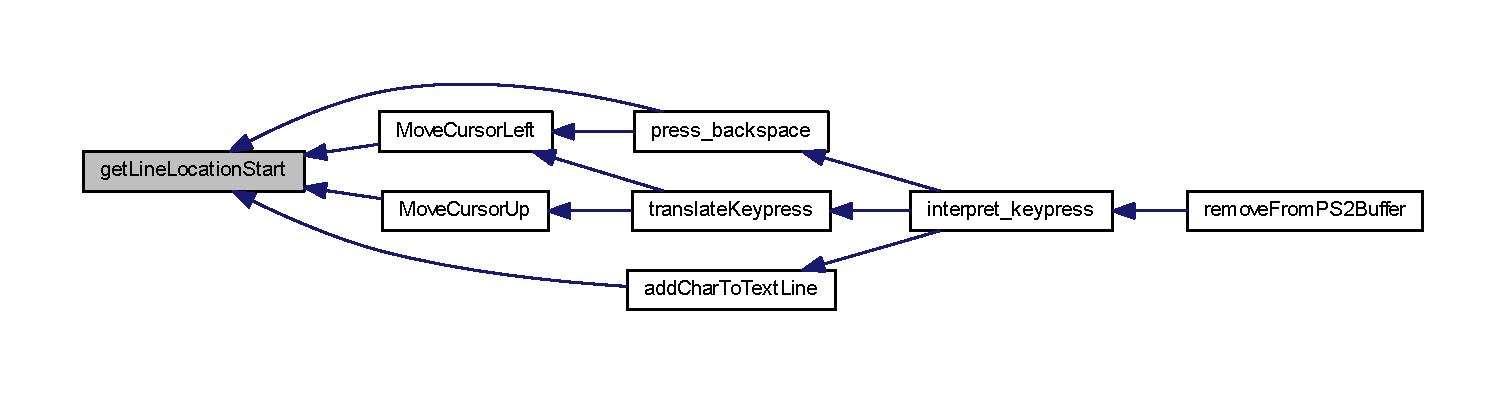
\includegraphics[width=350pt]{cursor_8h_a52e93559a57ee99d14ce6d275cbb47a6_icgraph}
\end{center}
\end{figure}


\hypertarget{cursor_8h_a3a060fca8f2dde6562e2f243414d47d7}{}\index{cursor.\+h@{cursor.\+h}!gettext\+Line@{gettext\+Line}}
\index{gettext\+Line@{gettext\+Line}!cursor.\+h@{cursor.\+h}}
\subsubsection[{gettext\+Line}]{\setlength{\rightskip}{0pt plus 5cm}uint8\+\_\+t$\ast$ gettext\+Line (
\begin{DoxyParamCaption}
\item[{void}]{}
\end{DoxyParamCaption}
)}\label{cursor_8h_a3a060fca8f2dde6562e2f243414d47d7}


Definition at line 506 of file cursor.\+c.

\hypertarget{cursor_8h_a06559067271121a8ba77c7e7f387a8f3}{}\index{cursor.\+h@{cursor.\+h}!increase\+Line\+Location\+End@{increase\+Line\+Location\+End}}
\index{increase\+Line\+Location\+End@{increase\+Line\+Location\+End}!cursor.\+h@{cursor.\+h}}
\subsubsection[{increase\+Line\+Location\+End}]{\setlength{\rightskip}{0pt plus 5cm}void increase\+Line\+Location\+End (
\begin{DoxyParamCaption}
\item[{void}]{}
\end{DoxyParamCaption}
)}\label{cursor_8h_a06559067271121a8ba77c7e7f387a8f3}


Definition at line 118 of file cursor.\+c.



Here is the caller graph for this function\+:\nopagebreak
\begin{figure}[H]
\begin{center}
\leavevmode
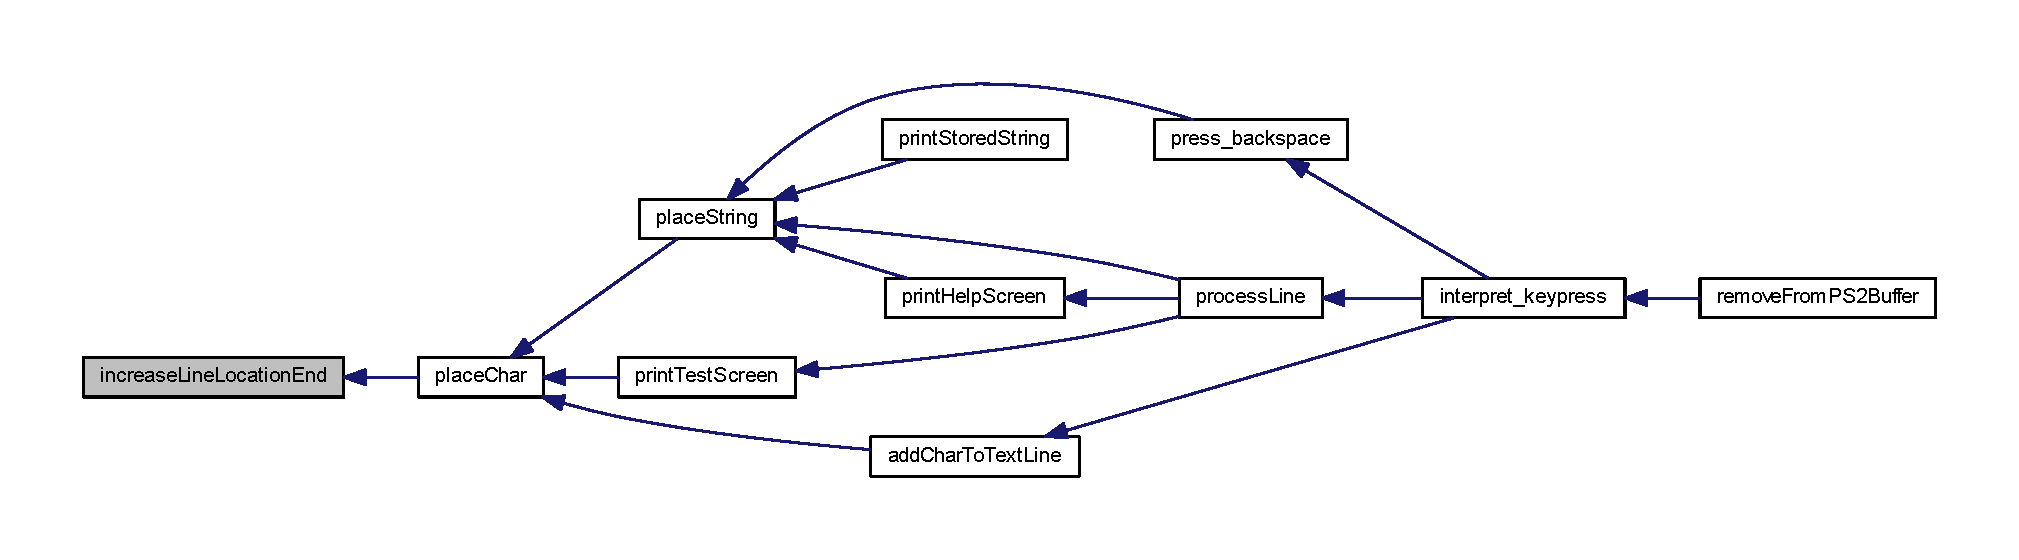
\includegraphics[width=350pt]{cursor_8h_a06559067271121a8ba77c7e7f387a8f3_icgraph}
\end{center}
\end{figure}


\hypertarget{cursor_8h_ad74454a9d14ccfe37bfa622791fa47e8}{}\index{cursor.\+h@{cursor.\+h}!increase\+Line\+Location\+End\+One\+Line@{increase\+Line\+Location\+End\+One\+Line}}
\index{increase\+Line\+Location\+End\+One\+Line@{increase\+Line\+Location\+End\+One\+Line}!cursor.\+h@{cursor.\+h}}
\subsubsection[{increase\+Line\+Location\+End\+One\+Line}]{\setlength{\rightskip}{0pt plus 5cm}void increase\+Line\+Location\+End\+One\+Line (
\begin{DoxyParamCaption}
\item[{void}]{}
\end{DoxyParamCaption}
)}\label{cursor_8h_ad74454a9d14ccfe37bfa622791fa47e8}


Definition at line 124 of file cursor.\+c.



Here is the caller graph for this function\+:\nopagebreak
\begin{figure}[H]
\begin{center}
\leavevmode
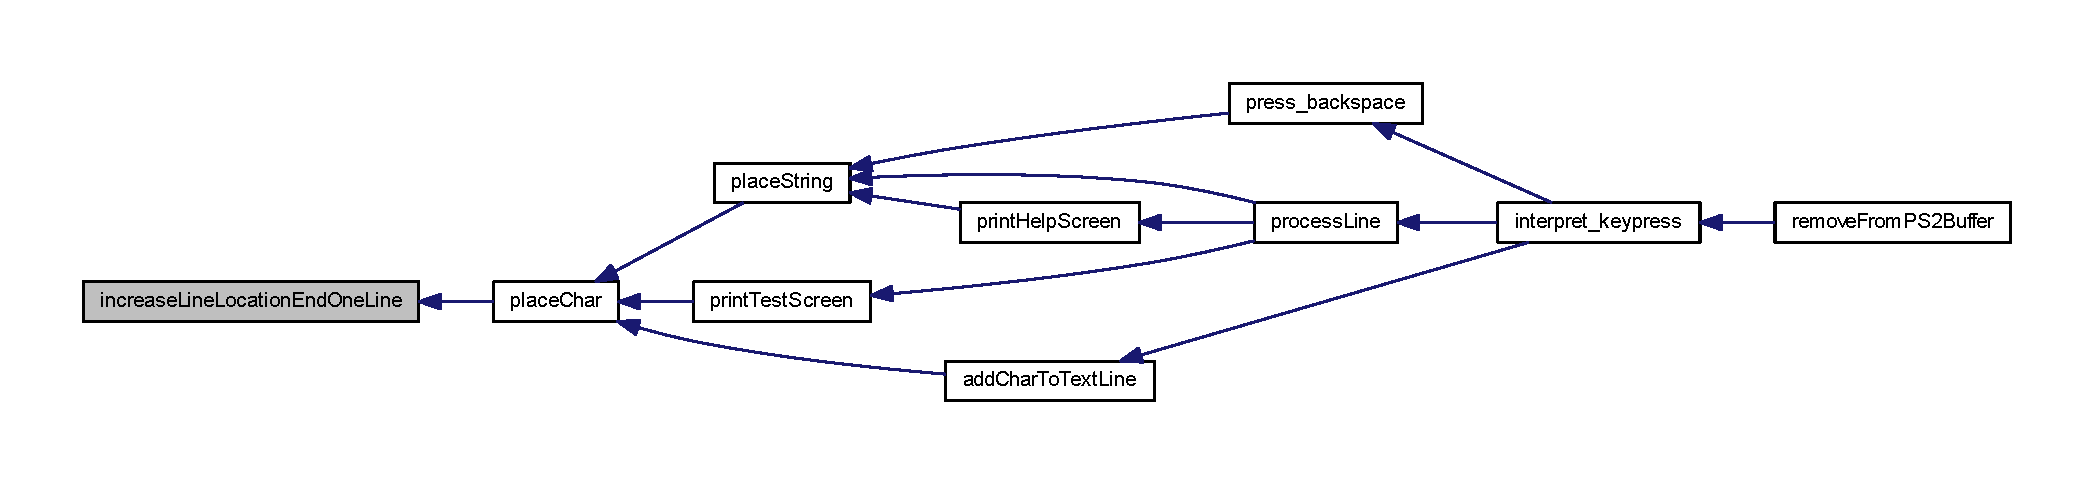
\includegraphics[width=350pt]{cursor_8h_ad74454a9d14ccfe37bfa622791fa47e8_icgraph}
\end{center}
\end{figure}


\hypertarget{cursor_8h_a467458fc0085539f52030fabf3dd9286}{}\index{cursor.\+h@{cursor.\+h}!interpret\+\_\+keypress@{interpret\+\_\+keypress}}
\index{interpret\+\_\+keypress@{interpret\+\_\+keypress}!cursor.\+h@{cursor.\+h}}
\subsubsection[{interpret\+\_\+keypress}]{\setlength{\rightskip}{0pt plus 5cm}void interpret\+\_\+keypress (
\begin{DoxyParamCaption}
\item[{char}]{temp}
\end{DoxyParamCaption}
)}\label{cursor_8h_a467458fc0085539f52030fabf3dd9286}


Definition at line 156 of file cursor.\+c.



Here is the call graph for this function\+:\nopagebreak
\begin{figure}[H]
\begin{center}
\leavevmode
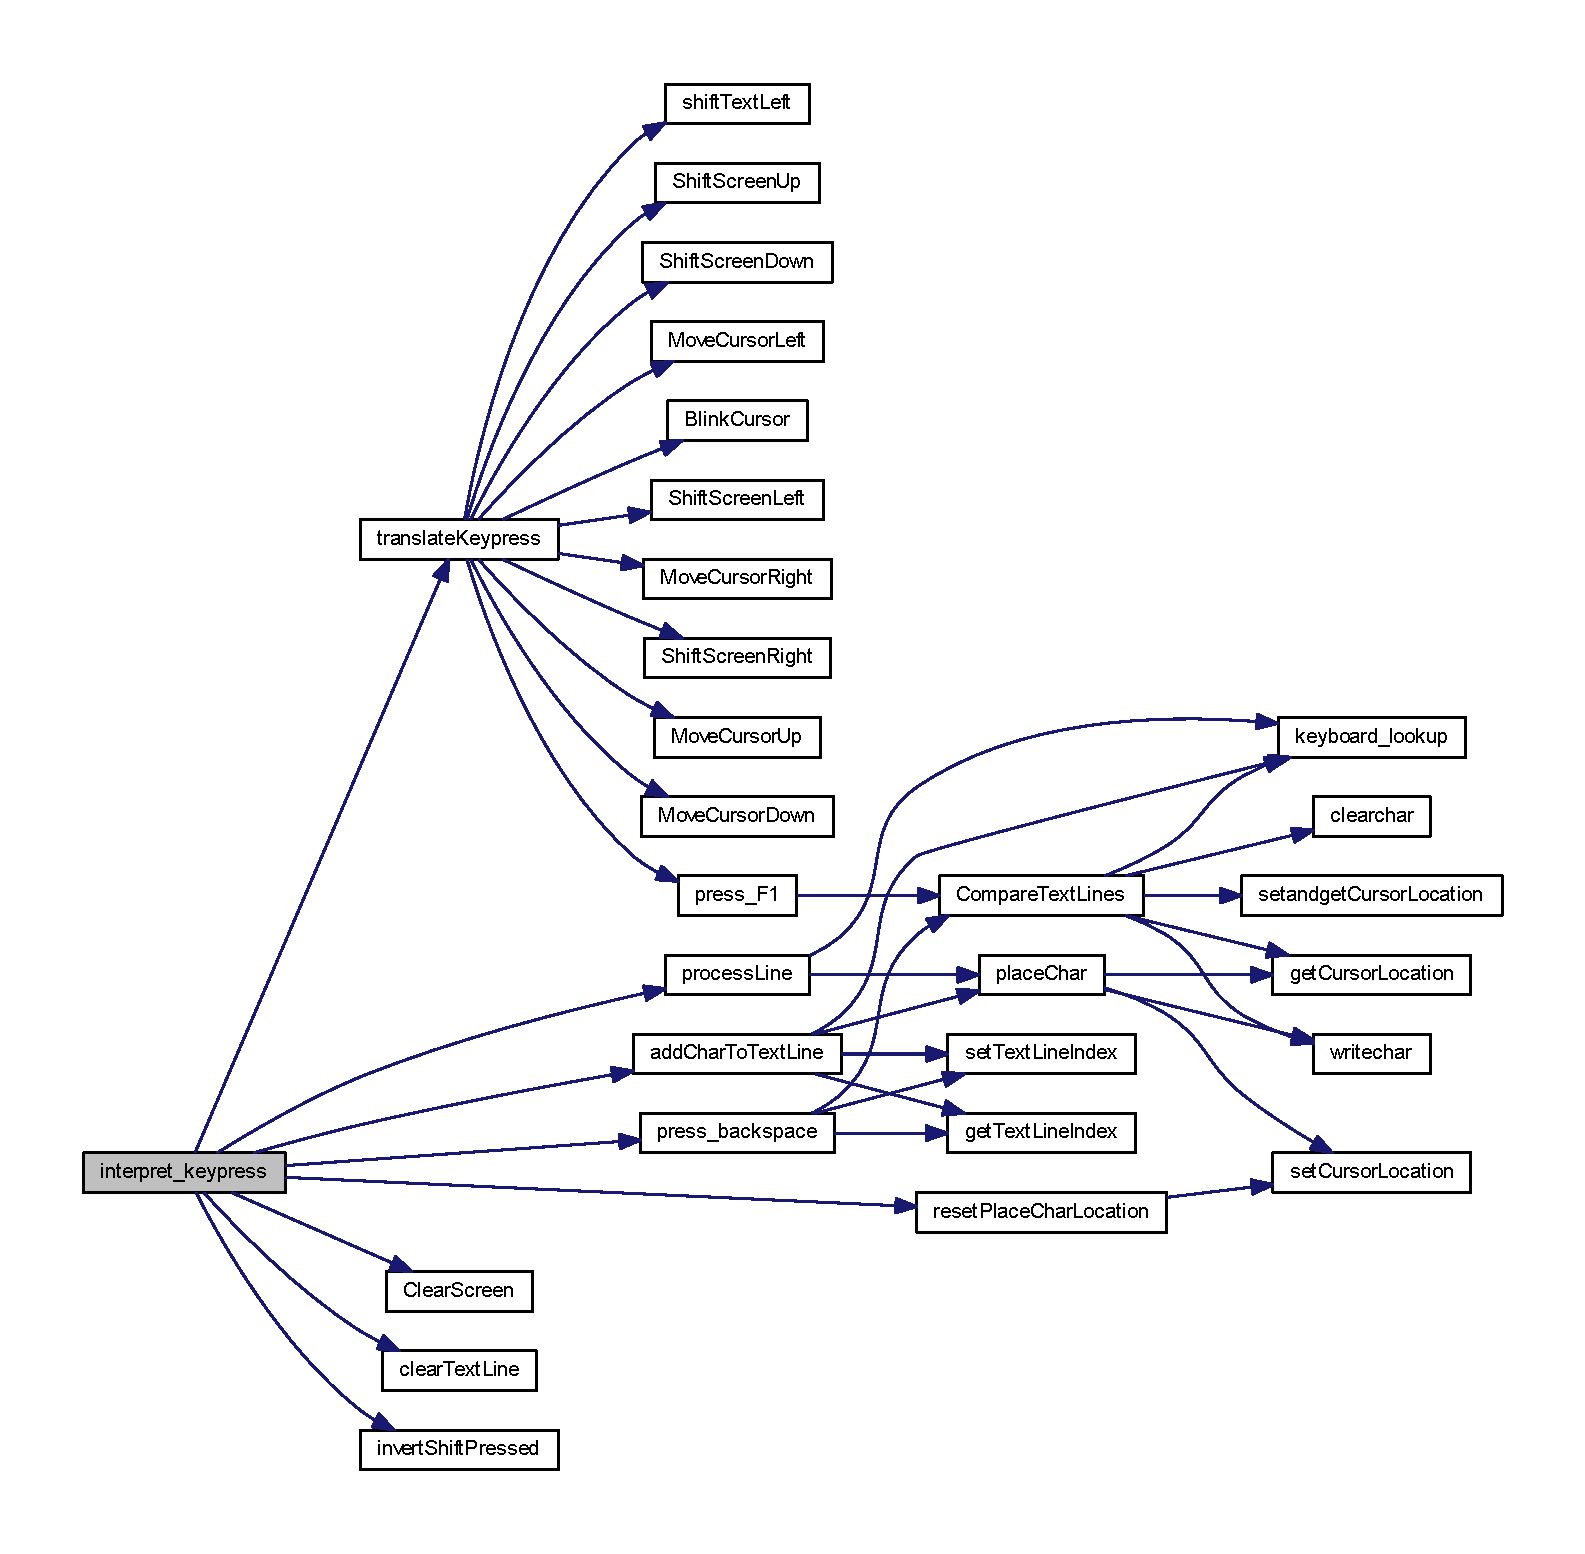
\includegraphics[width=350pt]{cursor_8h_a467458fc0085539f52030fabf3dd9286_cgraph}
\end{center}
\end{figure}




Here is the caller graph for this function\+:\nopagebreak
\begin{figure}[H]
\begin{center}
\leavevmode
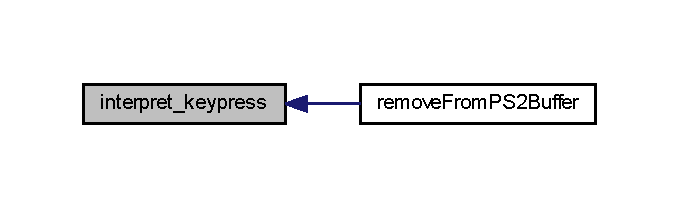
\includegraphics[width=326pt]{cursor_8h_a467458fc0085539f52030fabf3dd9286_icgraph}
\end{center}
\end{figure}


\hypertarget{cursor_8h_ac8e40e0b08b773c5f3fc0b303fe562de}{}\index{cursor.\+h@{cursor.\+h}!Move\+Cursor\+Down@{Move\+Cursor\+Down}}
\index{Move\+Cursor\+Down@{Move\+Cursor\+Down}!cursor.\+h@{cursor.\+h}}
\subsubsection[{Move\+Cursor\+Down}]{\setlength{\rightskip}{0pt plus 5cm}void Move\+Cursor\+Down (
\begin{DoxyParamCaption}
\item[{void}]{}
\end{DoxyParamCaption}
)}\label{cursor_8h_ac8e40e0b08b773c5f3fc0b303fe562de}


Definition at line 86 of file cursor.\+c.

\hypertarget{cursor_8h_aa0d5d4e3acd447e87fdab37d7388df23}{}\index{cursor.\+h@{cursor.\+h}!Move\+Cursor\+Down\+One\+Line@{Move\+Cursor\+Down\+One\+Line}}
\index{Move\+Cursor\+Down\+One\+Line@{Move\+Cursor\+Down\+One\+Line}!cursor.\+h@{cursor.\+h}}
\subsubsection[{Move\+Cursor\+Down\+One\+Line}]{\setlength{\rightskip}{0pt plus 5cm}void Move\+Cursor\+Down\+One\+Line (
\begin{DoxyParamCaption}
\item[{void}]{}
\end{DoxyParamCaption}
)}\label{cursor_8h_aa0d5d4e3acd447e87fdab37d7388df23}


Definition at line 102 of file cursor.\+c.



Here is the call graph for this function\+:\nopagebreak
\begin{figure}[H]
\begin{center}
\leavevmode
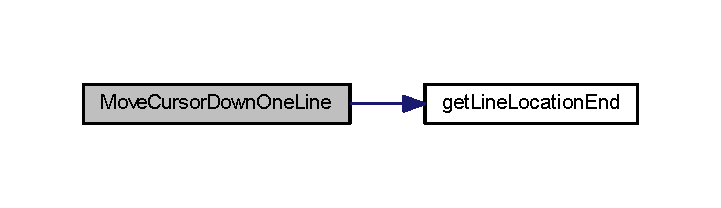
\includegraphics[width=346pt]{cursor_8h_aa0d5d4e3acd447e87fdab37d7388df23_cgraph}
\end{center}
\end{figure}




Here is the caller graph for this function\+:\nopagebreak
\begin{figure}[H]
\begin{center}
\leavevmode
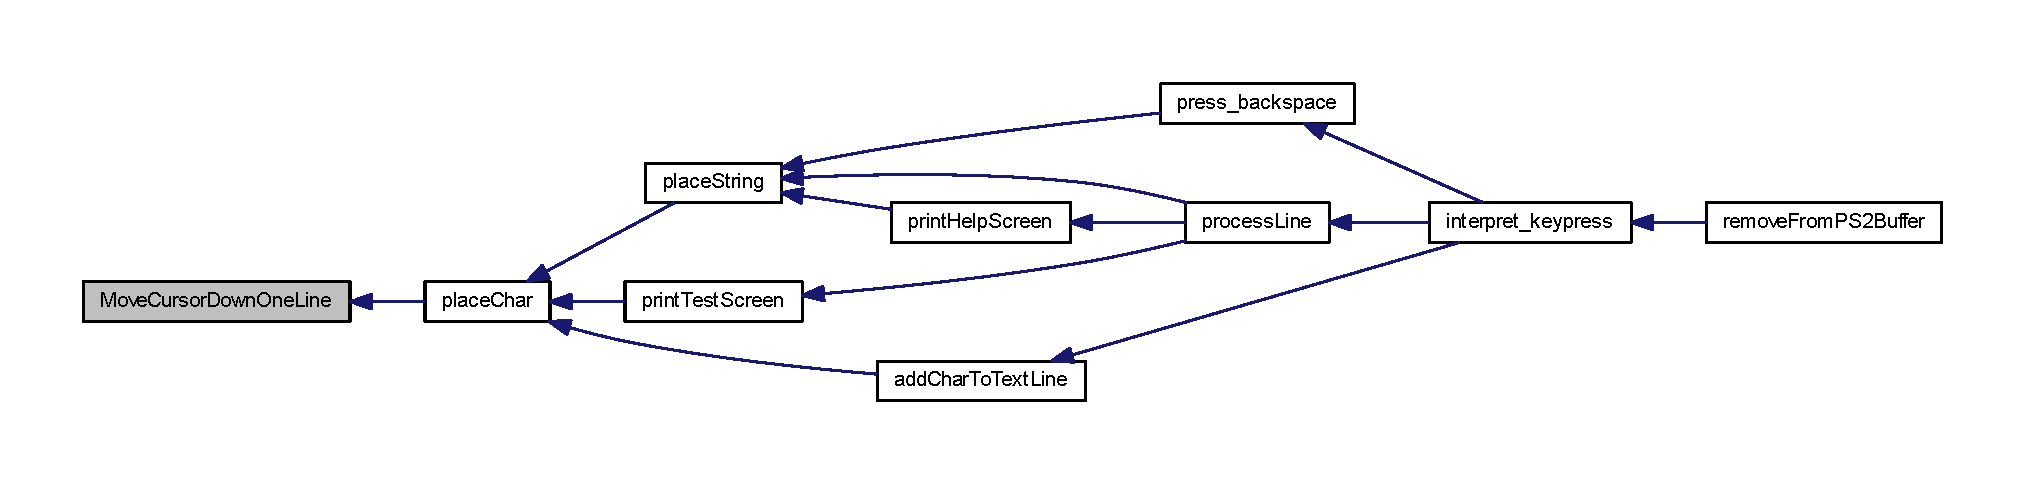
\includegraphics[width=350pt]{cursor_8h_aa0d5d4e3acd447e87fdab37d7388df23_icgraph}
\end{center}
\end{figure}


\hypertarget{cursor_8h_a7804524381705ec22e0efc3a1326dd69}{}\index{cursor.\+h@{cursor.\+h}!Move\+Cursor\+Left@{Move\+Cursor\+Left}}
\index{Move\+Cursor\+Left@{Move\+Cursor\+Left}!cursor.\+h@{cursor.\+h}}
\subsubsection[{Move\+Cursor\+Left}]{\setlength{\rightskip}{0pt plus 5cm}void Move\+Cursor\+Left (
\begin{DoxyParamCaption}
\item[{void}]{}
\end{DoxyParamCaption}
)}\label{cursor_8h_a7804524381705ec22e0efc3a1326dd69}


Definition at line 31 of file cursor.\+c.

\hypertarget{cursor_8h_ac177699cfeda15e4b887864f6eacc5e3}{}\index{cursor.\+h@{cursor.\+h}!Move\+Cursor\+Right@{Move\+Cursor\+Right}}
\index{Move\+Cursor\+Right@{Move\+Cursor\+Right}!cursor.\+h@{cursor.\+h}}
\subsubsection[{Move\+Cursor\+Right}]{\setlength{\rightskip}{0pt plus 5cm}void Move\+Cursor\+Right (
\begin{DoxyParamCaption}
\item[{void}]{}
\end{DoxyParamCaption}
)}\label{cursor_8h_ac177699cfeda15e4b887864f6eacc5e3}


Definition at line 53 of file cursor.\+c.

\hypertarget{cursor_8h_ae9337ec3c6ea47f10d329cd99d7a29f9}{}\index{cursor.\+h@{cursor.\+h}!Move\+Cursor\+Up@{Move\+Cursor\+Up}}
\index{Move\+Cursor\+Up@{Move\+Cursor\+Up}!cursor.\+h@{cursor.\+h}}
\subsubsection[{Move\+Cursor\+Up}]{\setlength{\rightskip}{0pt plus 5cm}void Move\+Cursor\+Up (
\begin{DoxyParamCaption}
\item[{void}]{}
\end{DoxyParamCaption}
)}\label{cursor_8h_ae9337ec3c6ea47f10d329cd99d7a29f9}


Definition at line 70 of file cursor.\+c.

\hypertarget{cursor_8h_a8d48f16d45338842dc6cbb3256eb7dae}{}\index{cursor.\+h@{cursor.\+h}!place\+Char@{place\+Char}}
\index{place\+Char@{place\+Char}!cursor.\+h@{cursor.\+h}}
\subsubsection[{place\+Char}]{\setlength{\rightskip}{0pt plus 5cm}void place\+Char (
\begin{DoxyParamCaption}
\item[{uint8\+\_\+t}]{character}
\end{DoxyParamCaption}
)}\label{cursor_8h_a8d48f16d45338842dc6cbb3256eb7dae}


Definition at line 455 of file cursor.\+c.



Here is the call graph for this function\+:\nopagebreak
\begin{figure}[H]
\begin{center}
\leavevmode
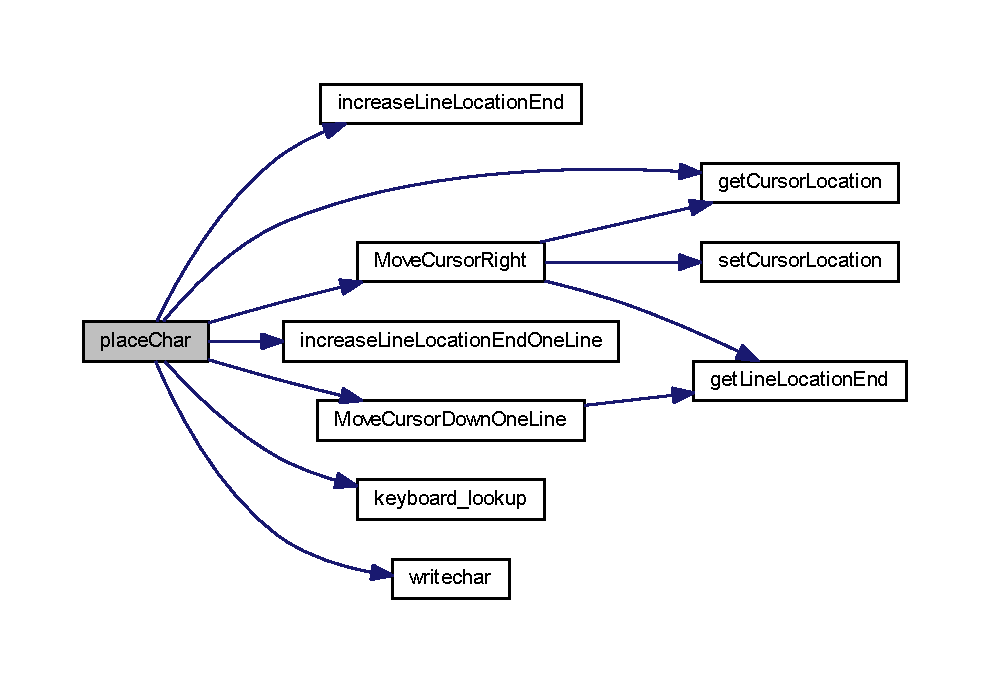
\includegraphics[width=350pt]{cursor_8h_a8d48f16d45338842dc6cbb3256eb7dae_cgraph}
\end{center}
\end{figure}




Here is the caller graph for this function\+:\nopagebreak
\begin{figure}[H]
\begin{center}
\leavevmode
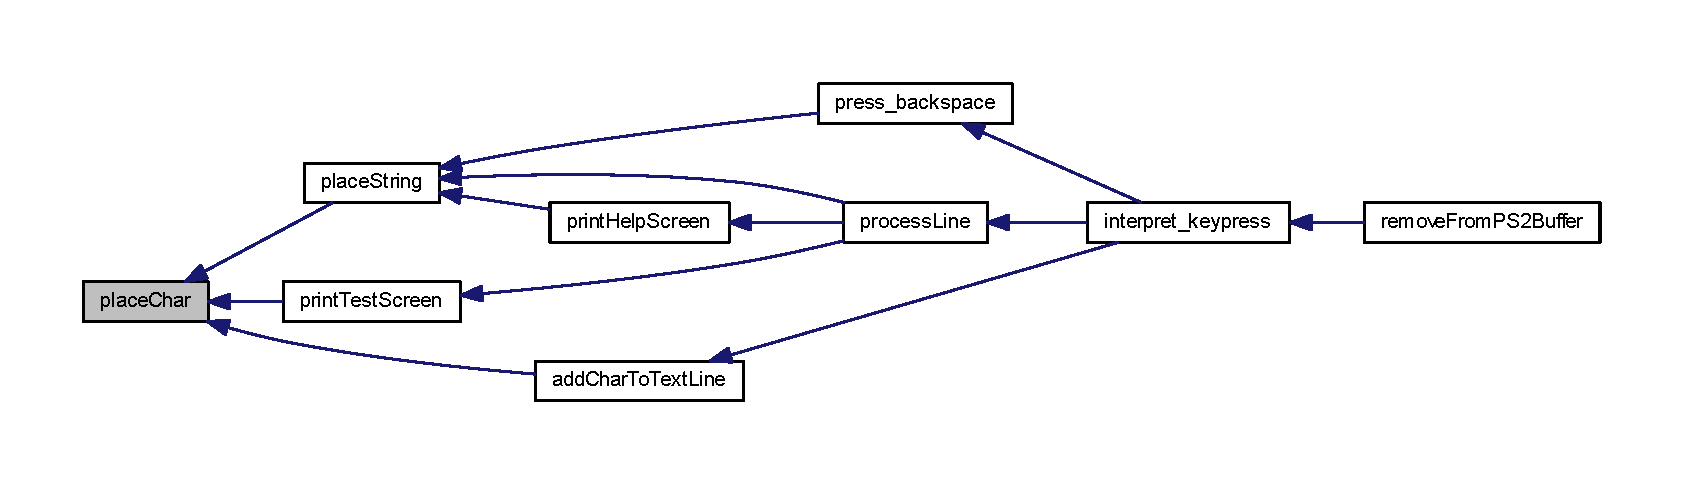
\includegraphics[width=350pt]{cursor_8h_a8d48f16d45338842dc6cbb3256eb7dae_icgraph}
\end{center}
\end{figure}


\hypertarget{cursor_8h_a02936826fc9c1380ef1e42ae18940c9a}{}\index{cursor.\+h@{cursor.\+h}!place\+String@{place\+String}}
\index{place\+String@{place\+String}!cursor.\+h@{cursor.\+h}}
\subsubsection[{place\+String}]{\setlength{\rightskip}{0pt plus 5cm}void place\+String (
\begin{DoxyParamCaption}
\item[{char $\ast$}]{string}
\end{DoxyParamCaption}
)}\label{cursor_8h_a02936826fc9c1380ef1e42ae18940c9a}
Places a null terminated string on the screen. 
\begin{DoxyParams}{Parameters}
{\em string} & -\/ string that gets placed on screen. \\
\hline
\end{DoxyParams}


Definition at line 444 of file cursor.\+c.



Here is the call graph for this function\+:\nopagebreak
\begin{figure}[H]
\begin{center}
\leavevmode
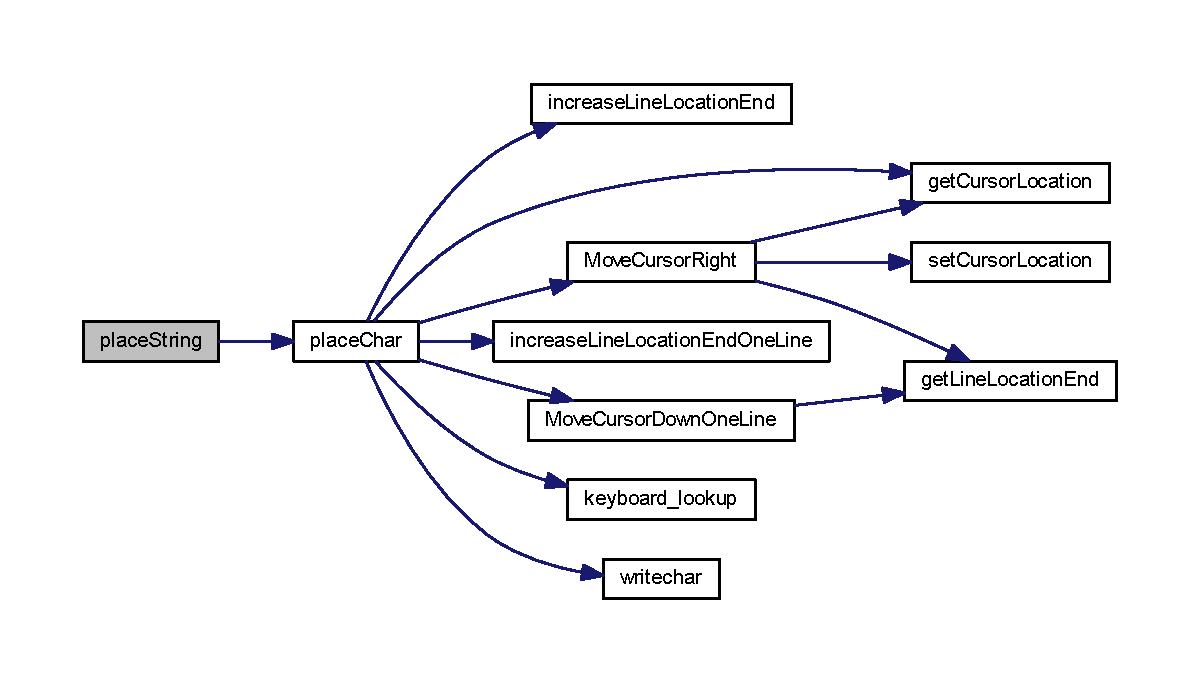
\includegraphics[width=350pt]{cursor_8h_a02936826fc9c1380ef1e42ae18940c9a_cgraph}
\end{center}
\end{figure}




Here is the caller graph for this function\+:\nopagebreak
\begin{figure}[H]
\begin{center}
\leavevmode
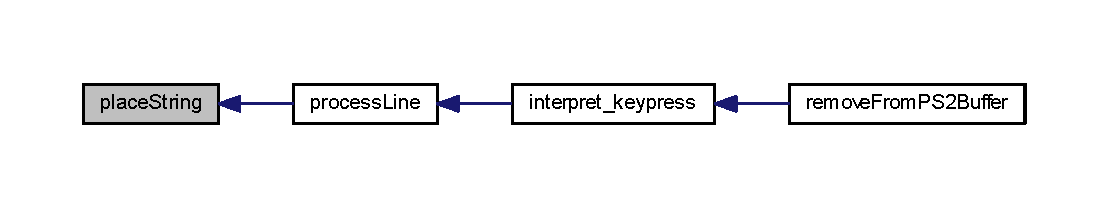
\includegraphics[width=350pt]{cursor_8h_a02936826fc9c1380ef1e42ae18940c9a_icgraph}
\end{center}
\end{figure}


\hypertarget{cursor_8h_afb368b3eb12755cae8787b96e467e0e3}{}\index{cursor.\+h@{cursor.\+h}!press\+\_\+backspace@{press\+\_\+backspace}}
\index{press\+\_\+backspace@{press\+\_\+backspace}!cursor.\+h@{cursor.\+h}}
\subsubsection[{press\+\_\+backspace}]{\setlength{\rightskip}{0pt plus 5cm}void press\+\_\+backspace (
\begin{DoxyParamCaption}
\item[{void}]{}
\end{DoxyParamCaption}
)}\label{cursor_8h_afb368b3eb12755cae8787b96e467e0e3}


Definition at line 336 of file cursor.\+c.



Here is the call graph for this function\+:\nopagebreak
\begin{figure}[H]
\begin{center}
\leavevmode
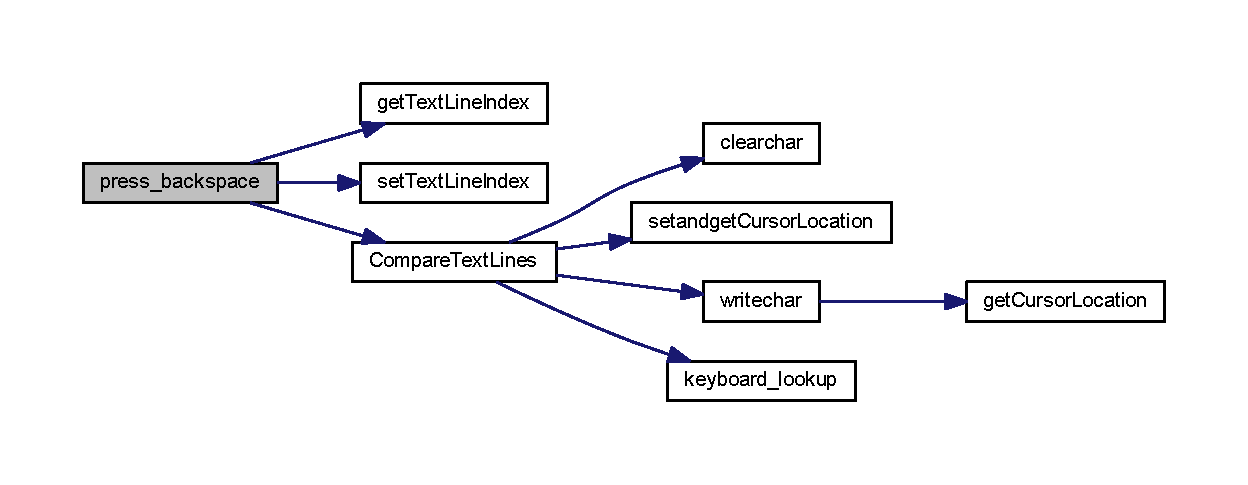
\includegraphics[width=350pt]{cursor_8h_afb368b3eb12755cae8787b96e467e0e3_cgraph}
\end{center}
\end{figure}




Here is the caller graph for this function\+:\nopagebreak
\begin{figure}[H]
\begin{center}
\leavevmode
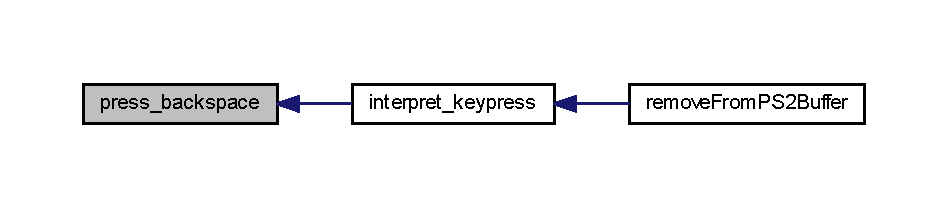
\includegraphics[width=350pt]{cursor_8h_afb368b3eb12755cae8787b96e467e0e3_icgraph}
\end{center}
\end{figure}


\hypertarget{cursor_8h_aa68556b6a4e7315e031e8f18361d283e}{}\index{cursor.\+h@{cursor.\+h}!print\+Help\+Screen@{print\+Help\+Screen}}
\index{print\+Help\+Screen@{print\+Help\+Screen}!cursor.\+h@{cursor.\+h}}
\subsubsection[{print\+Help\+Screen}]{\setlength{\rightskip}{0pt plus 5cm}void print\+Help\+Screen (
\begin{DoxyParamCaption}
\item[{void}]{}
\end{DoxyParamCaption}
)}\label{cursor_8h_aa68556b6a4e7315e031e8f18361d283e}


Definition at line 596 of file cursor.\+c.



Here is the call graph for this function\+:\nopagebreak
\begin{figure}[H]
\begin{center}
\leavevmode
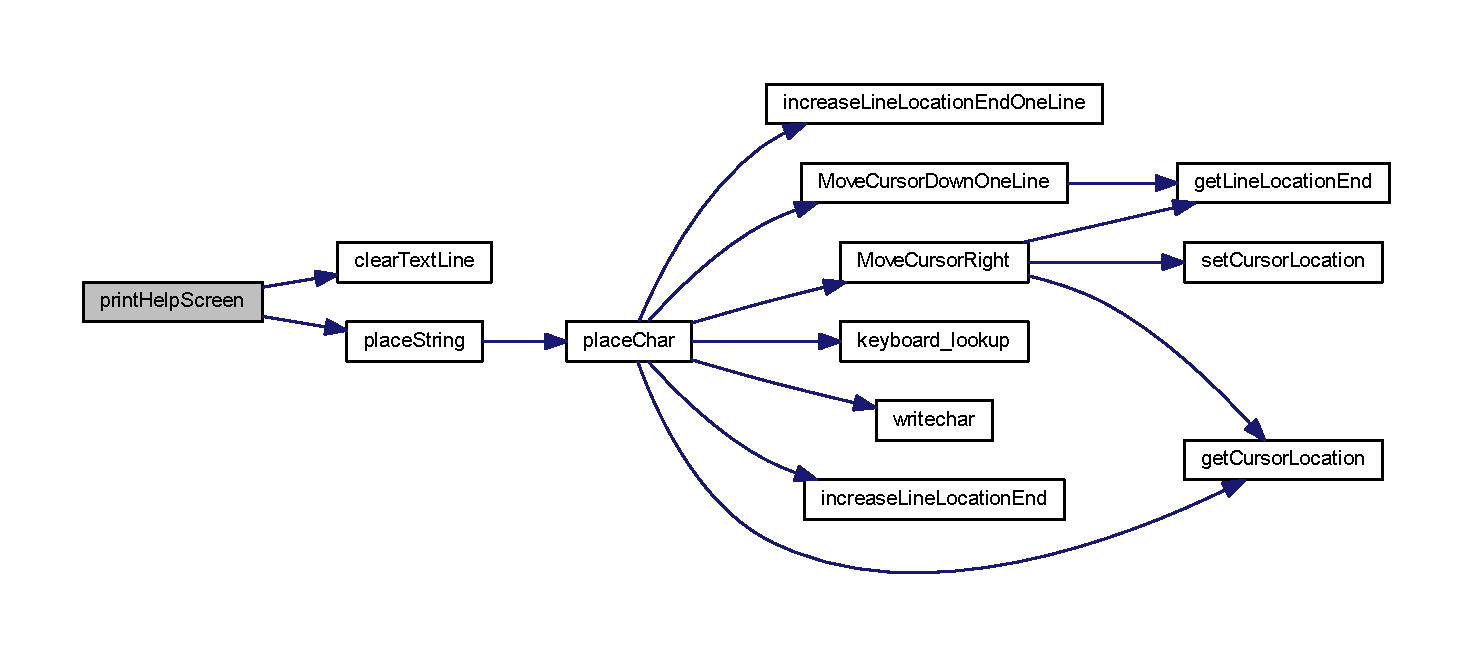
\includegraphics[width=350pt]{cursor_8h_aa68556b6a4e7315e031e8f18361d283e_cgraph}
\end{center}
\end{figure}




Here is the caller graph for this function\+:\nopagebreak
\begin{figure}[H]
\begin{center}
\leavevmode
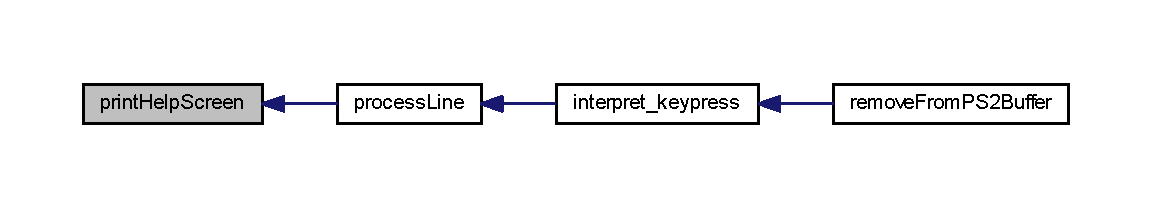
\includegraphics[width=350pt]{cursor_8h_aa68556b6a4e7315e031e8f18361d283e_icgraph}
\end{center}
\end{figure}


\hypertarget{cursor_8h_ab66a8865de62d9daefab9f8abf026478}{}\index{cursor.\+h@{cursor.\+h}!print\+Test\+Screen@{print\+Test\+Screen}}
\index{print\+Test\+Screen@{print\+Test\+Screen}!cursor.\+h@{cursor.\+h}}
\subsubsection[{print\+Test\+Screen}]{\setlength{\rightskip}{0pt plus 5cm}void print\+Test\+Screen (
\begin{DoxyParamCaption}
\item[{void}]{}
\end{DoxyParamCaption}
)}\label{cursor_8h_ab66a8865de62d9daefab9f8abf026478}


Definition at line 602 of file cursor.\+c.



Here is the call graph for this function\+:\nopagebreak
\begin{figure}[H]
\begin{center}
\leavevmode
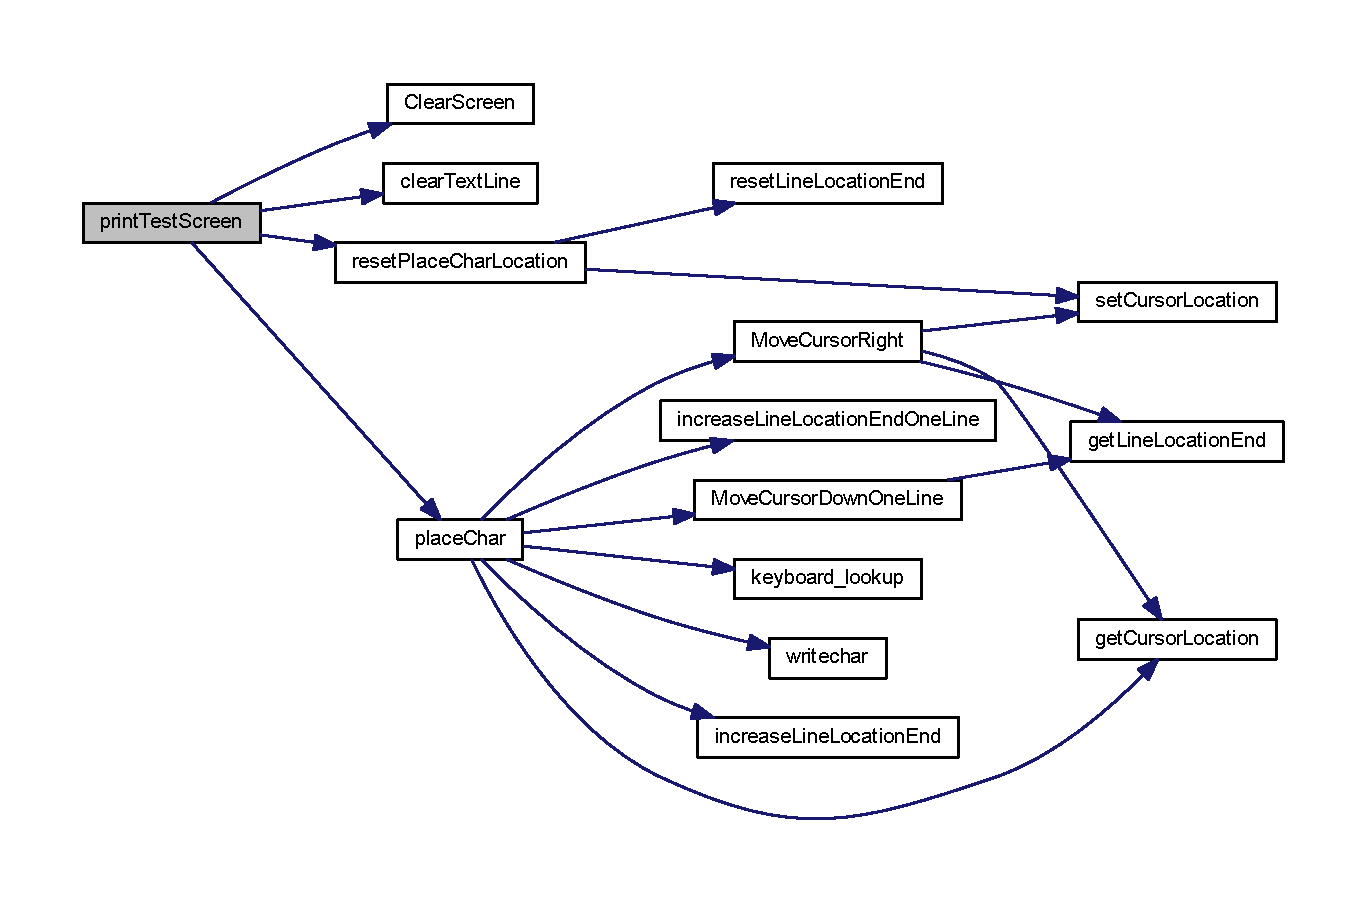
\includegraphics[width=350pt]{cursor_8h_ab66a8865de62d9daefab9f8abf026478_cgraph}
\end{center}
\end{figure}




Here is the caller graph for this function\+:\nopagebreak
\begin{figure}[H]
\begin{center}
\leavevmode
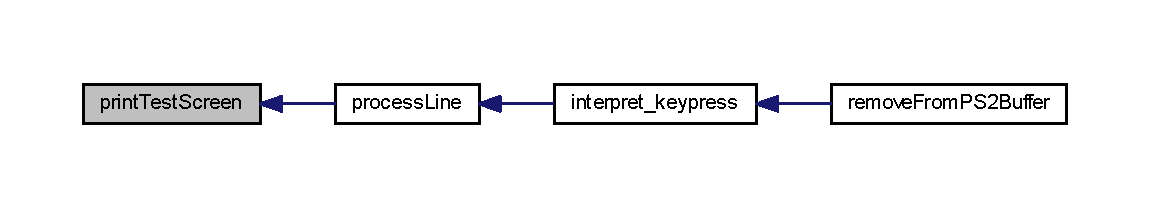
\includegraphics[width=350pt]{cursor_8h_ab66a8865de62d9daefab9f8abf026478_icgraph}
\end{center}
\end{figure}


\hypertarget{cursor_8h_aee82caceba560f01202c4459ba4497c7}{}\index{cursor.\+h@{cursor.\+h}!process\+Line@{process\+Line}}
\index{process\+Line@{process\+Line}!cursor.\+h@{cursor.\+h}}
\subsubsection[{process\+Line}]{\setlength{\rightskip}{0pt plus 5cm}void process\+Line (
\begin{DoxyParamCaption}
\item[{uint8\+\_\+t $\ast$}]{text\+Line\+Ptr}
\end{DoxyParamCaption}
)}\label{cursor_8h_aee82caceba560f01202c4459ba4497c7}


Definition at line 205 of file cursor.\+c.



Here is the call graph for this function\+:\nopagebreak
\begin{figure}[H]
\begin{center}
\leavevmode
\includegraphics[width=350pt]{cursor_8h_aee82caceba560f01202c4459ba4497c7_cgraph}
\end{center}
\end{figure}




Here is the caller graph for this function\+:\nopagebreak
\begin{figure}[H]
\begin{center}
\leavevmode
\includegraphics[width=350pt]{cursor_8h_aee82caceba560f01202c4459ba4497c7_icgraph}
\end{center}
\end{figure}


\hypertarget{cursor_8h_aeca62116778bb6c13245089867ded8d9}{}\index{cursor.\+h@{cursor.\+h}!reset\+Place\+Char\+Location@{reset\+Place\+Char\+Location}}
\index{reset\+Place\+Char\+Location@{reset\+Place\+Char\+Location}!cursor.\+h@{cursor.\+h}}
\subsubsection[{reset\+Place\+Char\+Location}]{\setlength{\rightskip}{0pt plus 5cm}void reset\+Place\+Char\+Location (
\begin{DoxyParamCaption}
\item[{void}]{}
\end{DoxyParamCaption}
)}\label{cursor_8h_aeca62116778bb6c13245089867ded8d9}


Definition at line 197 of file cursor.\+c.

\hypertarget{cursor_8h_a3a7d62c4f2983e6e2e2f4da56f36befc}{}\index{cursor.\+h@{cursor.\+h}!setandget\+Cursor\+Location@{setandget\+Cursor\+Location}}
\index{setandget\+Cursor\+Location@{setandget\+Cursor\+Location}!cursor.\+h@{cursor.\+h}}
\subsubsection[{setandget\+Cursor\+Location}]{\setlength{\rightskip}{0pt plus 5cm}int setandget\+Cursor\+Location (
\begin{DoxyParamCaption}
\item[{int}]{newcursor\+Location}
\end{DoxyParamCaption}
)}\label{cursor_8h_a3a7d62c4f2983e6e2e2f4da56f36befc}


Definition at line 6 of file cursor.\+c.



Here is the caller graph for this function\+:\nopagebreak
\begin{figure}[H]
\begin{center}
\leavevmode
\includegraphics[width=350pt]{cursor_8h_a3a7d62c4f2983e6e2e2f4da56f36befc_icgraph}
\end{center}
\end{figure}


\hypertarget{cursor_8h_acd4b06887a4337467e744f693a2df6a9}{}\index{cursor.\+h@{cursor.\+h}!set\+Cursor\+Location@{set\+Cursor\+Location}}
\index{set\+Cursor\+Location@{set\+Cursor\+Location}!cursor.\+h@{cursor.\+h}}
\subsubsection[{set\+Cursor\+Location}]{\setlength{\rightskip}{0pt plus 5cm}void set\+Cursor\+Location (
\begin{DoxyParamCaption}
\item[{int}]{new\+Cursor\+Location}
\end{DoxyParamCaption}
)}\label{cursor_8h_acd4b06887a4337467e744f693a2df6a9}
Sets the cursor location manually. Not suggested for normal use. No parameter checking. 
\begin{DoxyParams}{Parameters}
{\em new\+Cursor\+Location} & -\/ int that the cursor will be set to. \\
\hline
\end{DoxyParams}


Definition at line 26 of file cursor.\+c.



Here is the caller graph for this function\+:\nopagebreak
\begin{figure}[H]
\begin{center}
\leavevmode
\includegraphics[width=350pt]{cursor_8h_acd4b06887a4337467e744f693a2df6a9_icgraph}
\end{center}
\end{figure}


\hypertarget{cursor_8h_a453e2db022d7de17533e1509906065c9}{}\index{cursor.\+h@{cursor.\+h}!set\+Line\+Location\+Start@{set\+Line\+Location\+Start}}
\index{set\+Line\+Location\+Start@{set\+Line\+Location\+Start}!cursor.\+h@{cursor.\+h}}
\subsubsection[{set\+Line\+Location\+Start}]{\setlength{\rightskip}{0pt plus 5cm}void set\+Line\+Location\+Start (
\begin{DoxyParamCaption}
\item[{int}]{new\+Line\+Location\+Start}
\end{DoxyParamCaption}
)}\label{cursor_8h_a453e2db022d7de17533e1509906065c9}


Definition at line 150 of file cursor.\+c.



Here is the caller graph for this function\+:\nopagebreak
\begin{figure}[H]
\begin{center}
\leavevmode
\includegraphics[width=350pt]{cursor_8h_a453e2db022d7de17533e1509906065c9_icgraph}
\end{center}
\end{figure}




\subsection{Variable Documentation}
\hypertarget{cursor_8h_a06590bd84e8fca8ad5292a6e5ca50890}{}\index{cursor.\+h@{cursor.\+h}!Cursor\+Location@{Cursor\+Location}}
\index{Cursor\+Location@{Cursor\+Location}!cursor.\+h@{cursor.\+h}}
\subsubsection[{Cursor\+Location}]{\setlength{\rightskip}{0pt plus 5cm}int Cursor\+Location}\label{cursor_8h_a06590bd84e8fca8ad5292a6e5ca50890}


Definition at line 32 of file cursor.\+h.

\hypertarget{cursor_8h_aa4e0d20faf2f41acbf49d137715ba813}{}\index{cursor.\+h@{cursor.\+h}!I\+P\+Target@{I\+P\+Target}}
\index{I\+P\+Target@{I\+P\+Target}!cursor.\+h@{cursor.\+h}}
\subsubsection[{I\+P\+Target}]{\setlength{\rightskip}{0pt plus 5cm}char I\+P\+Target\mbox{[}16\mbox{]}}\label{cursor_8h_aa4e0d20faf2f41acbf49d137715ba813}


Definition at line 70 of file cursor.\+h.

\hypertarget{cursor_8h_a9edd5050c7ee33f44c008e98933880e0}{}\index{cursor.\+h@{cursor.\+h}!Line\+Location\+End@{Line\+Location\+End}}
\index{Line\+Location\+End@{Line\+Location\+End}!cursor.\+h@{cursor.\+h}}
\subsubsection[{Line\+Location\+End}]{\setlength{\rightskip}{0pt plus 5cm}int Line\+Location\+End}\label{cursor_8h_a9edd5050c7ee33f44c008e98933880e0}


Definition at line 37 of file cursor.\+h.

\hypertarget{cursor_8h_a96a71abb37405cb6ad878a4adac6d177}{}\index{cursor.\+h@{cursor.\+h}!Line\+Location\+Start@{Line\+Location\+Start}}
\index{Line\+Location\+Start@{Line\+Location\+Start}!cursor.\+h@{cursor.\+h}}
\subsubsection[{Line\+Location\+Start}]{\setlength{\rightskip}{0pt plus 5cm}int Line\+Location\+Start}\label{cursor_8h_a96a71abb37405cb6ad878a4adac6d177}


Definition at line 35 of file cursor.\+h.

\hypertarget{cursor_8h_a4eddb259269e1401df5b56698f231263}{}\index{cursor.\+h@{cursor.\+h}!newtext\+Line@{newtext\+Line}}
\index{newtext\+Line@{newtext\+Line}!cursor.\+h@{cursor.\+h}}
\subsubsection[{newtext\+Line}]{\setlength{\rightskip}{0pt plus 5cm}uint8\+\_\+t newtext\+Line\mbox{[}{\bf T\+E\+X\+T\+L\+I\+N\+E\+L\+E\+N\+G\+T\+H}\mbox{]}}\label{cursor_8h_a4eddb259269e1401df5b56698f231263}


Definition at line 80 of file cursor.\+h.

\hypertarget{cursor_8h_a78a502c5ea8364e4c06aea5ff4361c8f}{}\index{cursor.\+h@{cursor.\+h}!text\+Line@{text\+Line}}
\index{text\+Line@{text\+Line}!cursor.\+h@{cursor.\+h}}
\subsubsection[{text\+Line}]{\setlength{\rightskip}{0pt plus 5cm}uint8\+\_\+t text\+Line\mbox{[}{\bf T\+E\+X\+T\+L\+I\+N\+E\+L\+E\+N\+G\+T\+H}\mbox{]}}\label{cursor_8h_a78a502c5ea8364e4c06aea5ff4361c8f}


Definition at line 79 of file cursor.\+h.


\hypertarget{_p_s2_8c}{}\section{D\+:/\+School/\+Senior\+Project/\+Eth\+Kit\+T\+C\+P/\+Dev/\+P\+S2.c File Reference}
\label{_p_s2_8c}\index{D\+:/\+School/\+Senior\+Project/\+Eth\+Kit\+T\+C\+P/\+Dev/\+P\+S2.\+c@{D\+:/\+School/\+Senior\+Project/\+Eth\+Kit\+T\+C\+P/\+Dev/\+P\+S2.\+c}}
{\ttfamily \#include \char`\"{}P\+S2.\+h\char`\"{}}\\*
Include dependency graph for P\+S2.\+c\+:\nopagebreak
\begin{figure}[H]
\begin{center}
\leavevmode
\includegraphics[width=331pt]{_p_s2_8c__incl}
\end{center}
\end{figure}
\subsection*{Functions}
\begin{DoxyCompactItemize}
\item 
uint8\+\_\+t $\ast$ \hyperlink{_p_s2_8c_ae311e9417c9347d550643de4daea45e5}{keyboard\+\_\+lookup} (uint8\+\_\+t number)
\item 
void \hyperlink{_p_s2_8c_aab6a9276acf7260f4f6dfcd5a4c92e4a}{remove\+From\+P\+S2\+Buffer} (void)
\item 
uint8\+\_\+t \hyperlink{_p_s2_8c_a8ab149b8e337f892e4c07286e094ee54}{translate\+Keypress} (uint8\+\_\+t translate)
\item 
void \hyperlink{_p_s2_8c_a5391d4586620db9cb2c8e96627f37f7e}{test\+Keyboard\+Agitator} (uint8\+\_\+t scan\+Code)
\item 
void \hyperlink{_p_s2_8c_a6d4d2e35c21e102669b9fdf8a3858e99}{invert\+Shift\+Pressed} (void)
\end{DoxyCompactItemize}
\subsection*{Variables}
\begin{DoxyCompactItemize}
\item 
uint8\+\_\+t \hyperlink{_p_s2_8c_a7cda0ad58ffd2ffb3ab59b7cad3a947c}{font\+\_\+map} \mbox{[}128\mbox{]}\mbox{[}8\mbox{]}
\end{DoxyCompactItemize}


\subsection{Function Documentation}
\hypertarget{_p_s2_8c_a6d4d2e35c21e102669b9fdf8a3858e99}{}\index{P\+S2.\+c@{P\+S2.\+c}!invert\+Shift\+Pressed@{invert\+Shift\+Pressed}}
\index{invert\+Shift\+Pressed@{invert\+Shift\+Pressed}!P\+S2.\+c@{P\+S2.\+c}}
\subsubsection[{invert\+Shift\+Pressed}]{\setlength{\rightskip}{0pt plus 5cm}void invert\+Shift\+Pressed (
\begin{DoxyParamCaption}
\item[{void}]{}
\end{DoxyParamCaption}
)}\label{_p_s2_8c_a6d4d2e35c21e102669b9fdf8a3858e99}


Definition at line 1082 of file P\+S2.\+c.



Here is the caller graph for this function\+:\nopagebreak
\begin{figure}[H]
\begin{center}
\leavevmode
\includegraphics[width=350pt]{_p_s2_8c_a6d4d2e35c21e102669b9fdf8a3858e99_icgraph}
\end{center}
\end{figure}


\hypertarget{_p_s2_8c_ae311e9417c9347d550643de4daea45e5}{}\index{P\+S2.\+c@{P\+S2.\+c}!keyboard\+\_\+lookup@{keyboard\+\_\+lookup}}
\index{keyboard\+\_\+lookup@{keyboard\+\_\+lookup}!P\+S2.\+c@{P\+S2.\+c}}
\subsubsection[{keyboard\+\_\+lookup}]{\setlength{\rightskip}{0pt plus 5cm}uint8\+\_\+t$\ast$ keyboard\+\_\+lookup (
\begin{DoxyParamCaption}
\item[{uint8\+\_\+t}]{number}
\end{DoxyParamCaption}
)}\label{_p_s2_8c_ae311e9417c9347d550643de4daea45e5}
Checks if the keyboard scan code is within ascii range. If it is, it returns an 8x8 bitmap. 
\begin{DoxyParams}{Parameters}
{\em number} & -\/ Scan code to look up \\
\hline
\end{DoxyParams}
\begin{DoxyReturn}{Returns}
-\/ An 8 unit array of 8bit values that make an 8x8 bitmap 
\end{DoxyReturn}


Definition at line 143 of file P\+S2.\+c.



Here is the caller graph for this function\+:\nopagebreak
\begin{figure}[H]
\begin{center}
\leavevmode
\includegraphics[width=350pt]{_p_s2_8c_ae311e9417c9347d550643de4daea45e5_icgraph}
\end{center}
\end{figure}


\hypertarget{_p_s2_8c_aab6a9276acf7260f4f6dfcd5a4c92e4a}{}\index{P\+S2.\+c@{P\+S2.\+c}!remove\+From\+P\+S2\+Buffer@{remove\+From\+P\+S2\+Buffer}}
\index{remove\+From\+P\+S2\+Buffer@{remove\+From\+P\+S2\+Buffer}!P\+S2.\+c@{P\+S2.\+c}}
\subsubsection[{remove\+From\+P\+S2\+Buffer}]{\setlength{\rightskip}{0pt plus 5cm}void remove\+From\+P\+S2\+Buffer (
\begin{DoxyParamCaption}
\item[{void}]{}
\end{DoxyParamCaption}
)}\label{_p_s2_8c_aab6a9276acf7260f4f6dfcd5a4c92e4a}


Definition at line 295 of file P\+S2.\+c.



Here is the call graph for this function\+:\nopagebreak
\begin{figure}[H]
\begin{center}
\leavevmode
\includegraphics[width=350pt]{_p_s2_8c_aab6a9276acf7260f4f6dfcd5a4c92e4a_cgraph}
\end{center}
\end{figure}


\hypertarget{_p_s2_8c_a5391d4586620db9cb2c8e96627f37f7e}{}\index{P\+S2.\+c@{P\+S2.\+c}!test\+Keyboard\+Agitator@{test\+Keyboard\+Agitator}}
\index{test\+Keyboard\+Agitator@{test\+Keyboard\+Agitator}!P\+S2.\+c@{P\+S2.\+c}}
\subsubsection[{test\+Keyboard\+Agitator}]{\setlength{\rightskip}{0pt plus 5cm}void test\+Keyboard\+Agitator (
\begin{DoxyParamCaption}
\item[{uint8\+\_\+t}]{scan\+Code}
\end{DoxyParamCaption}
)}\label{_p_s2_8c_a5391d4586620db9cb2c8e96627f37f7e}


Definition at line 1058 of file P\+S2.\+c.

\hypertarget{_p_s2_8c_a8ab149b8e337f892e4c07286e094ee54}{}\index{P\+S2.\+c@{P\+S2.\+c}!translate\+Keypress@{translate\+Keypress}}
\index{translate\+Keypress@{translate\+Keypress}!P\+S2.\+c@{P\+S2.\+c}}
\subsubsection[{translate\+Keypress}]{\setlength{\rightskip}{0pt plus 5cm}uint8\+\_\+t translate\+Keypress (
\begin{DoxyParamCaption}
\item[{uint8\+\_\+t}]{translate}
\end{DoxyParamCaption}
)}\label{_p_s2_8c_a8ab149b8e337f892e4c07286e094ee54}


Definition at line 378 of file P\+S2.\+c.



Here is the call graph for this function\+:\nopagebreak
\begin{figure}[H]
\begin{center}
\leavevmode
\includegraphics[width=350pt]{_p_s2_8c_a8ab149b8e337f892e4c07286e094ee54_cgraph}
\end{center}
\end{figure}




Here is the caller graph for this function\+:\nopagebreak
\begin{figure}[H]
\begin{center}
\leavevmode
\includegraphics[width=350pt]{_p_s2_8c_a8ab149b8e337f892e4c07286e094ee54_icgraph}
\end{center}
\end{figure}




\subsection{Variable Documentation}
\hypertarget{_p_s2_8c_a7cda0ad58ffd2ffb3ab59b7cad3a947c}{}\index{P\+S2.\+c@{P\+S2.\+c}!font\+\_\+map@{font\+\_\+map}}
\index{font\+\_\+map@{font\+\_\+map}!P\+S2.\+c@{P\+S2.\+c}}
\subsubsection[{font\+\_\+map}]{\setlength{\rightskip}{0pt plus 5cm}uint8\+\_\+t font\+\_\+map\mbox{[}128\mbox{]}\mbox{[}8\mbox{]}}\label{_p_s2_8c_a7cda0ad58ffd2ffb3ab59b7cad3a947c}
A chunk of 128 8x8 bitmaps that are arranged in ascii order. 

Definition at line 6 of file P\+S2.\+c.


\hypertarget{_p_s2_8h}{}\section{D\+:/\+School/\+Senior\+Project/\+Eth\+Kit\+T\+C\+P/\+Dev/\+P\+S2.h File Reference}
\label{_p_s2_8h}\index{D\+:/\+School/\+Senior\+Project/\+Eth\+Kit\+T\+C\+P/\+Dev/\+P\+S2.\+h@{D\+:/\+School/\+Senior\+Project/\+Eth\+Kit\+T\+C\+P/\+Dev/\+P\+S2.\+h}}
{\ttfamily \#include $<$stdint.\+h$>$}\\*
{\ttfamily \#include \char`\"{}P\+S2\+Common.\+h\char`\"{}}\\*
{\ttfamily \#include \char`\"{}Test\+Common.\+h\char`\"{}}\\*
Include dependency graph for P\+S2.\+h\+:
% FIG 0
This graph shows which files directly or indirectly include this file\+:\nopagebreak
\begin{figure}[H]
\begin{center}
\leavevmode
\includegraphics[width=201pt]{_p_s2_8h__dep__incl}
\end{center}
\end{figure}
\subsection*{Macros}
\begin{DoxyCompactItemize}
\item 
\#define \hyperlink{_p_s2_8h_a4b8578b52cb39af2122c5047a8520757}{ps2\+Buffer\+Size}~100
\end{DoxyCompactItemize}
\subsection*{Functions}
\begin{DoxyCompactItemize}
\item 
void \hyperlink{_p_s2_8h_a6d4d2e35c21e102669b9fdf8a3858e99}{invert\+Shift\+Pressed} (void)
\item 
void \hyperlink{_p_s2_8h_a0f63d5a4267ee5aef23c951d50458049}{Temp\+Process\+Line\+Wrapper} (void)
\item 
uint8\+\_\+t $\ast$ \hyperlink{_p_s2_8h_ae311e9417c9347d550643de4daea45e5}{keyboard\+\_\+lookup} (uint8\+\_\+t number)
\item 
void \hyperlink{_p_s2_8h_a1c9949e161f05ecf2ba74181c4fdd1af}{keyboard\+\_\+setup} (void)
\item 
void \hyperlink{_p_s2_8h_aab6a9276acf7260f4f6dfcd5a4c92e4a}{remove\+From\+P\+S2\+Buffer} (void)
\item 
uint8\+\_\+t \hyperlink{_p_s2_8h_a01ddbbb07d07e31ed7bce301ba934d43}{translate\+Keypress} (uint8\+\_\+t)
\item 
void \hyperlink{_p_s2_8h_a467458fc0085539f52030fabf3dd9286}{interpret\+\_\+keypress} (char temp)
\item 
void \hyperlink{_p_s2_8h_a8d48f16d45338842dc6cbb3256eb7dae}{place\+Char} (uint8\+\_\+t character)
\item 
void \hyperlink{_p_s2_8h_a819307bdf0c8c8a841a2305637d102c2}{Shift\+Screen\+Up} (void)
\item 
void \hyperlink{_p_s2_8h_a030e6b6983ff846d9cca945c743c40b2}{Shift\+Screen\+Down} (void)
\item 
void \hyperlink{_p_s2_8h_a16432961ed8b60a6197456a6d92e4ddc}{Shift\+Screen\+Left} (void)
\item 
void \hyperlink{_p_s2_8h_a9c1bdbae316b73cb3580823f20c413f3}{Shift\+Screen\+Right} (void)
\item 
void \hyperlink{_p_s2_8h_a7804524381705ec22e0efc3a1326dd69}{Move\+Cursor\+Left} (void)
\item 
void \hyperlink{_p_s2_8h_ac177699cfeda15e4b887864f6eacc5e3}{Move\+Cursor\+Right} (void)
\item 
void \hyperlink{_p_s2_8h_ae9337ec3c6ea47f10d329cd99d7a29f9}{Move\+Cursor\+Up} (void)
\item 
void \hyperlink{_p_s2_8h_ac8e40e0b08b773c5f3fc0b303fe562de}{Move\+Cursor\+Down} (void)
\item 
void \hyperlink{_p_s2_8h_acea8175bc07b5d0ba9f3f78d0c00c4a7}{Blink\+Cursor} (void)
\item 
void \hyperlink{_p_s2_8h_a5473c6cfd6c580642133754e141ca556}{Clear\+Screen} (void)
\item 
void \hyperlink{_p_s2_8h_aeca62116778bb6c13245089867ded8d9}{reset\+Place\+Char\+Location} (void)
\item 
void \hyperlink{_p_s2_8h_a5391d4586620db9cb2c8e96627f37f7e}{test\+Keyboard\+Agitator} (uint8\+\_\+t scan\+Code)
\end{DoxyCompactItemize}
\subsection*{Variables}
\begin{DoxyCompactItemize}
\item 
int \hyperlink{_p_s2_8h_a2725544e7a06f2eb04622b77b3b57ac7}{values} \mbox{[}23\mbox{]}
\item 
int \hyperlink{_p_s2_8h_a54e2cac8504e2abd41419a6177c97344}{I\+C1\+State}
\item 
int \hyperlink{_p_s2_8h_ab100c3940bcc51c739758e8ab77b5330}{scancode}
\item 
int \hyperlink{_p_s2_8h_a7d0767b3a211317df10f5b01f5402d18}{ps2\+Buffer\+End\+Index}
\item 
int \hyperlink{_p_s2_8h_a8631eed927347d2af2042273a5e835e8}{ps2\+Buffer} \mbox{[}100\mbox{]}
\item 
int \hyperlink{_p_s2_8h_a4b47033f07f05416b1337b1c3469df6c}{Keys\+To\+Process}
\item 
int \hyperlink{_p_s2_8h_adb5fec5145465bea5af5eec1e194a1b7}{ps2\+Buffer\+Start}
\item 
int \hyperlink{_p_s2_8h_a6191505e87fa160d36f50dfb2f69233e}{ps2\+Buffer\+Num\+Items}
\item 
int \hyperlink{_p_s2_8h_a2083ba3e6f9cee8c4694d88b456e6d24}{Shift\+Pressed}
\item 
uint8\+\_\+t \hyperlink{_p_s2_8h_a7cda0ad58ffd2ffb3ab59b7cad3a947c}{font\+\_\+map} \mbox{[}128\mbox{]}\mbox{[}8\mbox{]}
\end{DoxyCompactItemize}


\subsection{Macro Definition Documentation}
\hypertarget{_p_s2_8h_a4b8578b52cb39af2122c5047a8520757}{}\index{P\+S2.\+h@{P\+S2.\+h}!ps2\+Buffer\+Size@{ps2\+Buffer\+Size}}
\index{ps2\+Buffer\+Size@{ps2\+Buffer\+Size}!P\+S2.\+h@{P\+S2.\+h}}
\subsubsection[{ps2\+Buffer\+Size}]{\setlength{\rightskip}{0pt plus 5cm}\#define ps2\+Buffer\+Size~100}\label{_p_s2_8h_a4b8578b52cb39af2122c5047a8520757}


Definition at line 49 of file P\+S2.\+h.



\subsection{Function Documentation}
\hypertarget{_p_s2_8h_acea8175bc07b5d0ba9f3f78d0c00c4a7}{}\index{P\+S2.\+h@{P\+S2.\+h}!Blink\+Cursor@{Blink\+Cursor}}
\index{Blink\+Cursor@{Blink\+Cursor}!P\+S2.\+h@{P\+S2.\+h}}
\subsubsection[{Blink\+Cursor}]{\setlength{\rightskip}{0pt plus 5cm}void Blink\+Cursor (
\begin{DoxyParamCaption}
\item[{void}]{}
\end{DoxyParamCaption}
)}\label{_p_s2_8h_acea8175bc07b5d0ba9f3f78d0c00c4a7}


Definition at line 493 of file V\+G\+A.\+c.



Here is the caller graph for this function\+:
% FIG 1


\hypertarget{_p_s2_8h_a5473c6cfd6c580642133754e141ca556}{}\index{P\+S2.\+h@{P\+S2.\+h}!Clear\+Screen@{Clear\+Screen}}
\index{Clear\+Screen@{Clear\+Screen}!P\+S2.\+h@{P\+S2.\+h}}
\subsubsection[{Clear\+Screen}]{\setlength{\rightskip}{0pt plus 5cm}void Clear\+Screen (
\begin{DoxyParamCaption}
\item[{void}]{}
\end{DoxyParamCaption}
)}\label{_p_s2_8h_a5473c6cfd6c580642133754e141ca556}
clears the entire screen 

Definition at line 481 of file V\+G\+A.\+c.



Here is the caller graph for this function\+:
% FIG 2


\hypertarget{_p_s2_8h_a467458fc0085539f52030fabf3dd9286}{}\index{P\+S2.\+h@{P\+S2.\+h}!interpret\+\_\+keypress@{interpret\+\_\+keypress}}
\index{interpret\+\_\+keypress@{interpret\+\_\+keypress}!P\+S2.\+h@{P\+S2.\+h}}
\subsubsection[{interpret\+\_\+keypress}]{\setlength{\rightskip}{0pt plus 5cm}void interpret\+\_\+keypress (
\begin{DoxyParamCaption}
\item[{char}]{temp}
\end{DoxyParamCaption}
)}\label{_p_s2_8h_a467458fc0085539f52030fabf3dd9286}


Definition at line 156 of file cursor.\+c.



Here is the call graph for this function\+:
% FIG 3




Here is the caller graph for this function\+:
% FIG 4


\hypertarget{_p_s2_8h_a6d4d2e35c21e102669b9fdf8a3858e99}{}\index{P\+S2.\+h@{P\+S2.\+h}!invert\+Shift\+Pressed@{invert\+Shift\+Pressed}}
\index{invert\+Shift\+Pressed@{invert\+Shift\+Pressed}!P\+S2.\+h@{P\+S2.\+h}}
\subsubsection[{invert\+Shift\+Pressed}]{\setlength{\rightskip}{0pt plus 5cm}void invert\+Shift\+Pressed (
\begin{DoxyParamCaption}
\item[{void}]{}
\end{DoxyParamCaption}
)}\label{_p_s2_8h_a6d4d2e35c21e102669b9fdf8a3858e99}


Definition at line 1088 of file P\+S2.\+c.



Here is the caller graph for this function\+:
% FIG 5


\hypertarget{_p_s2_8h_ae311e9417c9347d550643de4daea45e5}{}\index{P\+S2.\+h@{P\+S2.\+h}!keyboard\+\_\+lookup@{keyboard\+\_\+lookup}}
\index{keyboard\+\_\+lookup@{keyboard\+\_\+lookup}!P\+S2.\+h@{P\+S2.\+h}}
\subsubsection[{keyboard\+\_\+lookup}]{\setlength{\rightskip}{0pt plus 5cm}uint8\+\_\+t$\ast$ keyboard\+\_\+lookup (
\begin{DoxyParamCaption}
\item[{uint8\+\_\+t}]{number}
\end{DoxyParamCaption}
)}\label{_p_s2_8h_ae311e9417c9347d550643de4daea45e5}
Checks if the keyboard scan code is within ascii range. If it is, it returns an 8x8 bitmap. 
\begin{DoxyParams}{Parameters}
{\em number} & -\/ Scan code to look up \\
\hline
\end{DoxyParams}
\begin{DoxyReturn}{Returns}
-\/ An 8 unit array of 8bit values that make an 8x8 bitmap 
\end{DoxyReturn}


Definition at line 149 of file P\+S2.\+c.



Here is the caller graph for this function\+:
% FIG 6


\hypertarget{_p_s2_8h_a1c9949e161f05ecf2ba74181c4fdd1af}{}\index{P\+S2.\+h@{P\+S2.\+h}!keyboard\+\_\+setup@{keyboard\+\_\+setup}}
\index{keyboard\+\_\+setup@{keyboard\+\_\+setup}!P\+S2.\+h@{P\+S2.\+h}}
\subsubsection[{keyboard\+\_\+setup}]{\setlength{\rightskip}{0pt plus 5cm}void keyboard\+\_\+setup (
\begin{DoxyParamCaption}
\item[{void}]{}
\end{DoxyParamCaption}
)}\label{_p_s2_8h_a1c9949e161f05ecf2ba74181c4fdd1af}
\hypertarget{_p_s2_8h_ac8e40e0b08b773c5f3fc0b303fe562de}{}\index{P\+S2.\+h@{P\+S2.\+h}!Move\+Cursor\+Down@{Move\+Cursor\+Down}}
\index{Move\+Cursor\+Down@{Move\+Cursor\+Down}!P\+S2.\+h@{P\+S2.\+h}}
\subsubsection[{Move\+Cursor\+Down}]{\setlength{\rightskip}{0pt plus 5cm}void Move\+Cursor\+Down (
\begin{DoxyParamCaption}
\item[{void}]{}
\end{DoxyParamCaption}
)}\label{_p_s2_8h_ac8e40e0b08b773c5f3fc0b303fe562de}


Definition at line 86 of file cursor.\+c.



Here is the call graph for this function\+:\nopagebreak
\begin{figure}[H]
\begin{center}
\leavevmode
\includegraphics[width=310pt]{_p_s2_8h_ac8e40e0b08b773c5f3fc0b303fe562de_cgraph}
\end{center}
\end{figure}




Here is the caller graph for this function\+:
% FIG 7


\hypertarget{_p_s2_8h_a7804524381705ec22e0efc3a1326dd69}{}\index{P\+S2.\+h@{P\+S2.\+h}!Move\+Cursor\+Left@{Move\+Cursor\+Left}}
\index{Move\+Cursor\+Left@{Move\+Cursor\+Left}!P\+S2.\+h@{P\+S2.\+h}}
\subsubsection[{Move\+Cursor\+Left}]{\setlength{\rightskip}{0pt plus 5cm}void Move\+Cursor\+Left (
\begin{DoxyParamCaption}
\item[{void}]{}
\end{DoxyParamCaption}
)}\label{_p_s2_8h_a7804524381705ec22e0efc3a1326dd69}


Definition at line 31 of file cursor.\+c.



Here is the call graph for this function\+:\nopagebreak
\begin{figure}[H]
\begin{center}
\leavevmode
\includegraphics[width=305pt]{_p_s2_8h_a7804524381705ec22e0efc3a1326dd69_cgraph}
\end{center}
\end{figure}




Here is the caller graph for this function\+:
% FIG 8


\hypertarget{_p_s2_8h_ac177699cfeda15e4b887864f6eacc5e3}{}\index{P\+S2.\+h@{P\+S2.\+h}!Move\+Cursor\+Right@{Move\+Cursor\+Right}}
\index{Move\+Cursor\+Right@{Move\+Cursor\+Right}!P\+S2.\+h@{P\+S2.\+h}}
\subsubsection[{Move\+Cursor\+Right}]{\setlength{\rightskip}{0pt plus 5cm}void Move\+Cursor\+Right (
\begin{DoxyParamCaption}
\item[{void}]{}
\end{DoxyParamCaption}
)}\label{_p_s2_8h_ac177699cfeda15e4b887864f6eacc5e3}


Definition at line 53 of file cursor.\+c.



Here is the call graph for this function\+:\nopagebreak
\begin{figure}[H]
\begin{center}
\leavevmode
\includegraphics[width=308pt]{_p_s2_8h_ac177699cfeda15e4b887864f6eacc5e3_cgraph}
\end{center}
\end{figure}




Here is the caller graph for this function\+:
% FIG 9


\hypertarget{_p_s2_8h_ae9337ec3c6ea47f10d329cd99d7a29f9}{}\index{P\+S2.\+h@{P\+S2.\+h}!Move\+Cursor\+Up@{Move\+Cursor\+Up}}
\index{Move\+Cursor\+Up@{Move\+Cursor\+Up}!P\+S2.\+h@{P\+S2.\+h}}
\subsubsection[{Move\+Cursor\+Up}]{\setlength{\rightskip}{0pt plus 5cm}void Move\+Cursor\+Up (
\begin{DoxyParamCaption}
\item[{void}]{}
\end{DoxyParamCaption}
)}\label{_p_s2_8h_ae9337ec3c6ea47f10d329cd99d7a29f9}


Definition at line 70 of file cursor.\+c.



Here is the call graph for this function\+:\nopagebreak
\begin{figure}[H]
\begin{center}
\leavevmode
\includegraphics[width=302pt]{_p_s2_8h_ae9337ec3c6ea47f10d329cd99d7a29f9_cgraph}
\end{center}
\end{figure}




Here is the caller graph for this function\+:
% FIG 10


\hypertarget{_p_s2_8h_a8d48f16d45338842dc6cbb3256eb7dae}{}\index{P\+S2.\+h@{P\+S2.\+h}!place\+Char@{place\+Char}}
\index{place\+Char@{place\+Char}!P\+S2.\+h@{P\+S2.\+h}}
\subsubsection[{place\+Char}]{\setlength{\rightskip}{0pt plus 5cm}void place\+Char (
\begin{DoxyParamCaption}
\item[{uint8\+\_\+t}]{character}
\end{DoxyParamCaption}
)}\label{_p_s2_8h_a8d48f16d45338842dc6cbb3256eb7dae}


Definition at line 456 of file cursor.\+c.



Here is the call graph for this function\+:\nopagebreak
\begin{figure}[H]
\begin{center}
\leavevmode
\includegraphics[width=350pt]{_p_s2_8h_a8d48f16d45338842dc6cbb3256eb7dae_cgraph}
\end{center}
\end{figure}




Here is the caller graph for this function\+:
% FIG 11


\hypertarget{_p_s2_8h_aab6a9276acf7260f4f6dfcd5a4c92e4a}{}\index{P\+S2.\+h@{P\+S2.\+h}!remove\+From\+P\+S2\+Buffer@{remove\+From\+P\+S2\+Buffer}}
\index{remove\+From\+P\+S2\+Buffer@{remove\+From\+P\+S2\+Buffer}!P\+S2.\+h@{P\+S2.\+h}}
\subsubsection[{remove\+From\+P\+S2\+Buffer}]{\setlength{\rightskip}{0pt plus 5cm}void remove\+From\+P\+S2\+Buffer (
\begin{DoxyParamCaption}
\item[{void}]{}
\end{DoxyParamCaption}
)}\label{_p_s2_8h_aab6a9276acf7260f4f6dfcd5a4c92e4a}


Definition at line 301 of file P\+S2.\+c.



Here is the call graph for this function\+:
% FIG 12


\hypertarget{_p_s2_8h_aeca62116778bb6c13245089867ded8d9}{}\index{P\+S2.\+h@{P\+S2.\+h}!reset\+Place\+Char\+Location@{reset\+Place\+Char\+Location}}
\index{reset\+Place\+Char\+Location@{reset\+Place\+Char\+Location}!P\+S2.\+h@{P\+S2.\+h}}
\subsubsection[{reset\+Place\+Char\+Location}]{\setlength{\rightskip}{0pt plus 5cm}void reset\+Place\+Char\+Location (
\begin{DoxyParamCaption}
\item[{void}]{}
\end{DoxyParamCaption}
)}\label{_p_s2_8h_aeca62116778bb6c13245089867ded8d9}


Definition at line 197 of file cursor.\+c.



Here is the call graph for this function\+:\nopagebreak
\begin{figure}[H]
\begin{center}
\leavevmode
\includegraphics[width=346pt]{_p_s2_8h_aeca62116778bb6c13245089867ded8d9_cgraph}
\end{center}
\end{figure}




Here is the caller graph for this function\+:
% FIG 13


\hypertarget{_p_s2_8h_a030e6b6983ff846d9cca945c743c40b2}{}\index{P\+S2.\+h@{P\+S2.\+h}!Shift\+Screen\+Down@{Shift\+Screen\+Down}}
\index{Shift\+Screen\+Down@{Shift\+Screen\+Down}!P\+S2.\+h@{P\+S2.\+h}}
\subsubsection[{Shift\+Screen\+Down}]{\setlength{\rightskip}{0pt plus 5cm}void Shift\+Screen\+Down (
\begin{DoxyParamCaption}
\item[{void}]{}
\end{DoxyParamCaption}
)}\label{_p_s2_8h_a030e6b6983ff846d9cca945c743c40b2}


Definition at line 548 of file V\+G\+A.\+c.



Here is the caller graph for this function\+:
% FIG 14


\hypertarget{_p_s2_8h_a16432961ed8b60a6197456a6d92e4ddc}{}\index{P\+S2.\+h@{P\+S2.\+h}!Shift\+Screen\+Left@{Shift\+Screen\+Left}}
\index{Shift\+Screen\+Left@{Shift\+Screen\+Left}!P\+S2.\+h@{P\+S2.\+h}}
\subsubsection[{Shift\+Screen\+Left}]{\setlength{\rightskip}{0pt plus 5cm}void Shift\+Screen\+Left (
\begin{DoxyParamCaption}
\item[{void}]{}
\end{DoxyParamCaption}
)}\label{_p_s2_8h_a16432961ed8b60a6197456a6d92e4ddc}


Definition at line 574 of file V\+G\+A.\+c.



Here is the caller graph for this function\+:
% FIG 15


\hypertarget{_p_s2_8h_a9c1bdbae316b73cb3580823f20c413f3}{}\index{P\+S2.\+h@{P\+S2.\+h}!Shift\+Screen\+Right@{Shift\+Screen\+Right}}
\index{Shift\+Screen\+Right@{Shift\+Screen\+Right}!P\+S2.\+h@{P\+S2.\+h}}
\subsubsection[{Shift\+Screen\+Right}]{\setlength{\rightskip}{0pt plus 5cm}void Shift\+Screen\+Right (
\begin{DoxyParamCaption}
\item[{void}]{}
\end{DoxyParamCaption}
)}\label{_p_s2_8h_a9c1bdbae316b73cb3580823f20c413f3}


Definition at line 601 of file V\+G\+A.\+c.



Here is the caller graph for this function\+:
% FIG 16


\hypertarget{_p_s2_8h_a819307bdf0c8c8a841a2305637d102c2}{}\index{P\+S2.\+h@{P\+S2.\+h}!Shift\+Screen\+Up@{Shift\+Screen\+Up}}
\index{Shift\+Screen\+Up@{Shift\+Screen\+Up}!P\+S2.\+h@{P\+S2.\+h}}
\subsubsection[{Shift\+Screen\+Up}]{\setlength{\rightskip}{0pt plus 5cm}void Shift\+Screen\+Up (
\begin{DoxyParamCaption}
\item[{void}]{}
\end{DoxyParamCaption}
)}\label{_p_s2_8h_a819307bdf0c8c8a841a2305637d102c2}


Definition at line 522 of file V\+G\+A.\+c.



Here is the caller graph for this function\+:
% FIG 17


\hypertarget{_p_s2_8h_a0f63d5a4267ee5aef23c951d50458049}{}\index{P\+S2.\+h@{P\+S2.\+h}!Temp\+Process\+Line\+Wrapper@{Temp\+Process\+Line\+Wrapper}}
\index{Temp\+Process\+Line\+Wrapper@{Temp\+Process\+Line\+Wrapper}!P\+S2.\+h@{P\+S2.\+h}}
\subsubsection[{Temp\+Process\+Line\+Wrapper}]{\setlength{\rightskip}{0pt plus 5cm}void Temp\+Process\+Line\+Wrapper (
\begin{DoxyParamCaption}
\item[{void}]{}
\end{DoxyParamCaption}
)}\label{_p_s2_8h_a0f63d5a4267ee5aef23c951d50458049}
\hypertarget{_p_s2_8h_a5391d4586620db9cb2c8e96627f37f7e}{}\index{P\+S2.\+h@{P\+S2.\+h}!test\+Keyboard\+Agitator@{test\+Keyboard\+Agitator}}
\index{test\+Keyboard\+Agitator@{test\+Keyboard\+Agitator}!P\+S2.\+h@{P\+S2.\+h}}
\subsubsection[{test\+Keyboard\+Agitator}]{\setlength{\rightskip}{0pt plus 5cm}void test\+Keyboard\+Agitator (
\begin{DoxyParamCaption}
\item[{uint8\+\_\+t}]{scan\+Code}
\end{DoxyParamCaption}
)}\label{_p_s2_8h_a5391d4586620db9cb2c8e96627f37f7e}


Definition at line 1064 of file P\+S2.\+c.

\hypertarget{_p_s2_8h_a01ddbbb07d07e31ed7bce301ba934d43}{}\index{P\+S2.\+h@{P\+S2.\+h}!translate\+Keypress@{translate\+Keypress}}
\index{translate\+Keypress@{translate\+Keypress}!P\+S2.\+h@{P\+S2.\+h}}
\subsubsection[{translate\+Keypress}]{\setlength{\rightskip}{0pt plus 5cm}uint8\+\_\+t translate\+Keypress (
\begin{DoxyParamCaption}
\item[{uint8\+\_\+t}]{}
\end{DoxyParamCaption}
)}\label{_p_s2_8h_a01ddbbb07d07e31ed7bce301ba934d43}


Definition at line 384 of file P\+S2.\+c.



Here is the call graph for this function\+:
% FIG 18




Here is the caller graph for this function\+:
% FIG 19




\subsection{Variable Documentation}
\hypertarget{_p_s2_8h_a7cda0ad58ffd2ffb3ab59b7cad3a947c}{}\index{P\+S2.\+h@{P\+S2.\+h}!font\+\_\+map@{font\+\_\+map}}
\index{font\+\_\+map@{font\+\_\+map}!P\+S2.\+h@{P\+S2.\+h}}
\subsubsection[{font\+\_\+map}]{\setlength{\rightskip}{0pt plus 5cm}uint8\+\_\+t font\+\_\+map\mbox{[}128\mbox{]}\mbox{[}8\mbox{]}}\label{_p_s2_8h_a7cda0ad58ffd2ffb3ab59b7cad3a947c}
font\+\_\+map based on the file \href{http://users.ices.utexas.edu/~lenharth/cs378/fall13/font8x8.h}{\tt http\+://users.\+ices.\+utexas.\+edu/$\sim$lenharth/cs378/fall13/font8x8.\+h} released with comments below\+:

8x8 monochrome bitmap fonts for rendering Author\+: Daniel Hepper \href{mailto:daniel@hepper.net}{\tt daniel@hepper.\+net}

License\+: Public Domain

Based on\+: // Summary\+: font8x8.\+h // 8x8 monochrome bitmap fonts for rendering // // Author\+: // Marcel Sondaar // International Business Machines (public domain V\+G\+A fonts) // // License\+: // Public Domain

Fetched from\+: \href{http://dimensionalrift.homelinux.net/combuster/mos3/?p=viewsource&file=/modules/gfx/font8_8.asm}{\tt http\+://dimensionalrift.\+homelinux.\+net/combuster/mos3/?p=viewsource\&file=/modules/gfx/font8\+\_\+8.\+asm}

A chunk of 128 8x8 bitmaps that are arranged in ascii order. 

Definition at line 12 of file P\+S2.\+c.

\hypertarget{_p_s2_8h_a54e2cac8504e2abd41419a6177c97344}{}\index{P\+S2.\+h@{P\+S2.\+h}!I\+C1\+State@{I\+C1\+State}}
\index{I\+C1\+State@{I\+C1\+State}!P\+S2.\+h@{P\+S2.\+h}}
\subsubsection[{I\+C1\+State}]{\setlength{\rightskip}{0pt plus 5cm}int I\+C1\+State}\label{_p_s2_8h_a54e2cac8504e2abd41419a6177c97344}


Definition at line 37 of file P\+S2.\+h.

\hypertarget{_p_s2_8h_a4b47033f07f05416b1337b1c3469df6c}{}\index{P\+S2.\+h@{P\+S2.\+h}!Keys\+To\+Process@{Keys\+To\+Process}}
\index{Keys\+To\+Process@{Keys\+To\+Process}!P\+S2.\+h@{P\+S2.\+h}}
\subsubsection[{Keys\+To\+Process}]{\setlength{\rightskip}{0pt plus 5cm}int Keys\+To\+Process}\label{_p_s2_8h_a4b47033f07f05416b1337b1c3469df6c}
flag to communicate between the ps2 interrupt and the main loop key interpreting 

Definition at line 43 of file P\+S2.\+h.

\hypertarget{_p_s2_8h_a8631eed927347d2af2042273a5e835e8}{}\index{P\+S2.\+h@{P\+S2.\+h}!ps2\+Buffer@{ps2\+Buffer}}
\index{ps2\+Buffer@{ps2\+Buffer}!P\+S2.\+h@{P\+S2.\+h}}
\subsubsection[{ps2\+Buffer}]{\setlength{\rightskip}{0pt plus 5cm}int ps2\+Buffer\mbox{[}100\mbox{]}}\label{_p_s2_8h_a8631eed927347d2af2042273a5e835e8}


Definition at line 40 of file P\+S2.\+h.

\hypertarget{_p_s2_8h_a7d0767b3a211317df10f5b01f5402d18}{}\index{P\+S2.\+h@{P\+S2.\+h}!ps2\+Buffer\+End\+Index@{ps2\+Buffer\+End\+Index}}
\index{ps2\+Buffer\+End\+Index@{ps2\+Buffer\+End\+Index}!P\+S2.\+h@{P\+S2.\+h}}
\subsubsection[{ps2\+Buffer\+End\+Index}]{\setlength{\rightskip}{0pt plus 5cm}int ps2\+Buffer\+End\+Index}\label{_p_s2_8h_a7d0767b3a211317df10f5b01f5402d18}


Definition at line 39 of file P\+S2.\+h.

\hypertarget{_p_s2_8h_a6191505e87fa160d36f50dfb2f69233e}{}\index{P\+S2.\+h@{P\+S2.\+h}!ps2\+Buffer\+Num\+Items@{ps2\+Buffer\+Num\+Items}}
\index{ps2\+Buffer\+Num\+Items@{ps2\+Buffer\+Num\+Items}!P\+S2.\+h@{P\+S2.\+h}}
\subsubsection[{ps2\+Buffer\+Num\+Items}]{\setlength{\rightskip}{0pt plus 5cm}int ps2\+Buffer\+Num\+Items}\label{_p_s2_8h_a6191505e87fa160d36f50dfb2f69233e}


Definition at line 50 of file P\+S2.\+h.

\hypertarget{_p_s2_8h_adb5fec5145465bea5af5eec1e194a1b7}{}\index{P\+S2.\+h@{P\+S2.\+h}!ps2\+Buffer\+Start@{ps2\+Buffer\+Start}}
\index{ps2\+Buffer\+Start@{ps2\+Buffer\+Start}!P\+S2.\+h@{P\+S2.\+h}}
\subsubsection[{ps2\+Buffer\+Start}]{\setlength{\rightskip}{0pt plus 5cm}int ps2\+Buffer\+Start}\label{_p_s2_8h_adb5fec5145465bea5af5eec1e194a1b7}


Definition at line 47 of file P\+S2.\+h.

\hypertarget{_p_s2_8h_ab100c3940bcc51c739758e8ab77b5330}{}\index{P\+S2.\+h@{P\+S2.\+h}!scancode@{scancode}}
\index{scancode@{scancode}!P\+S2.\+h@{P\+S2.\+h}}
\subsubsection[{scancode}]{\setlength{\rightskip}{0pt plus 5cm}int scancode}\label{_p_s2_8h_ab100c3940bcc51c739758e8ab77b5330}


Definition at line 38 of file P\+S2.\+h.

\hypertarget{_p_s2_8h_a2083ba3e6f9cee8c4694d88b456e6d24}{}\index{P\+S2.\+h@{P\+S2.\+h}!Shift\+Pressed@{Shift\+Pressed}}
\index{Shift\+Pressed@{Shift\+Pressed}!P\+S2.\+h@{P\+S2.\+h}}
\subsubsection[{Shift\+Pressed}]{\setlength{\rightskip}{0pt plus 5cm}int Shift\+Pressed}\label{_p_s2_8h_a2083ba3e6f9cee8c4694d88b456e6d24}


Definition at line 53 of file P\+S2.\+h.

\hypertarget{_p_s2_8h_a2725544e7a06f2eb04622b77b3b57ac7}{}\index{P\+S2.\+h@{P\+S2.\+h}!values@{values}}
\index{values@{values}!P\+S2.\+h@{P\+S2.\+h}}
\subsubsection[{values}]{\setlength{\rightskip}{0pt plus 5cm}int values\mbox{[}23\mbox{]}}\label{_p_s2_8h_a2725544e7a06f2eb04622b77b3b57ac7}


Definition at line 36 of file P\+S2.\+h.


\hypertarget{_p_s2_common_8h}{}\section{C\+:/\+Users/mainuser/\+Desktop/\+School/\+Senior\+Project/\+Eth\+Kit\+T\+C\+P/\+Dev/\+P\+S2\+Common.h File Reference}
\label{_p_s2_common_8h}\index{C\+:/\+Users/mainuser/\+Desktop/\+School/\+Senior\+Project/\+Eth\+Kit\+T\+C\+P/\+Dev/\+P\+S2\+Common.\+h@{C\+:/\+Users/mainuser/\+Desktop/\+School/\+Senior\+Project/\+Eth\+Kit\+T\+C\+P/\+Dev/\+P\+S2\+Common.\+h}}
This graph shows which files directly or indirectly include this file\+:\nopagebreak
\begin{figure}[H]
\begin{center}
\leavevmode
\includegraphics[width=240pt]{_p_s2_common_8h__dep__incl}
\end{center}
\end{figure}
\subsection*{Variables}
\begin{DoxyCompactItemize}
\item 
int \hyperlink{_p_s2_common_8h_a4b47033f07f05416b1337b1c3469df6c}{Keys\+To\+Process}
\end{DoxyCompactItemize}


\subsection{Variable Documentation}
\hypertarget{_p_s2_common_8h_a4b47033f07f05416b1337b1c3469df6c}{}\index{P\+S2\+Common.\+h@{P\+S2\+Common.\+h}!Keys\+To\+Process@{Keys\+To\+Process}}
\index{Keys\+To\+Process@{Keys\+To\+Process}!P\+S2\+Common.\+h@{P\+S2\+Common.\+h}}
\subsubsection[{Keys\+To\+Process}]{\setlength{\rightskip}{0pt plus 5cm}int Keys\+To\+Process}\label{_p_s2_common_8h_a4b47033f07f05416b1337b1c3469df6c}


Definition at line 40 of file P\+S2.\+h.


\hypertarget{_test_common_8h}{}\section{D\+:/\+School/\+Senior\+Project/\+Eth\+Kit\+T\+C\+P/\+Dev/\+Test\+Common.h File Reference}
\label{_test_common_8h}\index{D\+:/\+School/\+Senior\+Project/\+Eth\+Kit\+T\+C\+P/\+Dev/\+Test\+Common.\+h@{D\+:/\+School/\+Senior\+Project/\+Eth\+Kit\+T\+C\+P/\+Dev/\+Test\+Common.\+h}}
This graph shows which files directly or indirectly include this file\+:\nopagebreak
\begin{figure}[H]
\begin{center}
\leavevmode
\includegraphics[width=350pt]{_test_common_8h__dep__incl}
\end{center}
\end{figure}

\hypertarget{_v_g_a_8c}{}\section{D\+:/\+School/\+Senior\+Project/\+Eth\+Kit\+T\+C\+P/\+Dev/\+V\+G\+A.c File Reference}
\label{_v_g_a_8c}\index{D\+:/\+School/\+Senior\+Project/\+Eth\+Kit\+T\+C\+P/\+Dev/\+V\+G\+A.\+c@{D\+:/\+School/\+Senior\+Project/\+Eth\+Kit\+T\+C\+P/\+Dev/\+V\+G\+A.\+c}}
{\ttfamily \#include \char`\"{}V\+G\+A.\+h\char`\"{}}\\*
Include dependency graph for V\+G\+A.\+c\+:\nopagebreak
\begin{figure}[H]
\begin{center}
\leavevmode
\includegraphics[width=230pt]{_v_g_a_8c__incl}
\end{center}
\end{figure}
\subsection*{Functions}
\begin{DoxyCompactItemize}
\item 
uint32\+\_\+t \hyperlink{_v_g_a_8c_a70a1baebed80d9631cc4a999fc3cda5d}{\+\_\+bswap32} (uint32\+\_\+t a)
\item 
void \hyperlink{_v_g_a_8c_a404c4fd746b185b08d63449a9c14049c}{writefullhorizontalline} (int line)
\item 
void \hyperlink{_v_g_a_8c_aa99b12cab66ebdbdf0d5b9c2e00a9c15}{writefullverticalline} (int column)
\item 
void \hyperlink{_v_g_a_8c_a822a698d29ce7edb349352481b65db74}{writehorizontalline} (int y1, int y2)
\item 
void \hyperlink{_v_g_a_8c_a0058c3096abb8e78f7ab293ab42daff8}{writeverticalline} (int x1, int x2)
\item 
void \hyperlink{_v_g_a_8c_ad6061cbae4f54062026bae527e5dee9a}{writepixel} (int x, int y)
\item 
void \hyperlink{_v_g_a_8c_a499c31fd29b2bb4509a35860bde799b6}{writechar} (uint8\+\_\+t $\ast$character, int x, int y)
\item 
void \hyperlink{_v_g_a_8c_a62abd37a46e00ef5754e42fdd601cb9f}{clearchar} (int start, int end)
\item 
void \hyperlink{_v_g_a_8c_a5473c6cfd6c580642133754e141ca556}{Clear\+Screen} (void)
\item 
void \hyperlink{_v_g_a_8c_acea8175bc07b5d0ba9f3f78d0c00c4a7}{Blink\+Cursor} (void)
\item 
void \hyperlink{_v_g_a_8c_ac087c08f80c03fa662b95603afbe19eb}{Shift\+Screen\+Up} ()
\item 
void \hyperlink{_v_g_a_8c_a7658a533b49674fdef8006fdcf6a694b}{Shift\+Screen\+Down} ()
\item 
void \hyperlink{_v_g_a_8c_ac1761d7d3dfc7d3514362f41649c1e93}{Shift\+Screen\+Left} ()
\item 
void \hyperlink{_v_g_a_8c_a3468671ccd9c43681712ba1cd515a7f0}{Shift\+Screen\+Right} ()
\item 
void \hyperlink{_v_g_a_8c_ab5c64bd9429e61e28c56cc7b35fb1f88}{shift\+Text\+Right} (void)
\item 
void \hyperlink{_v_g_a_8c_a1ff9068d637ee1bf5b357186033e3623}{shift\+Text\+Left} (void)
\end{DoxyCompactItemize}
\subsection*{Variables}
\begin{DoxyCompactItemize}
\item 
const long int \hyperlink{_v_g_a_8c_a64539db1fe3ee5a5aee9c5e8ea5b151c}{V\+G\+A\+\_\+\+Back\+Porch} \mbox{[}10\mbox{]} = \{0, 0, 0, 0, 0, 0, 0, 0, 0, 0\}
\end{DoxyCompactItemize}


\subsection{Function Documentation}
\hypertarget{_v_g_a_8c_a70a1baebed80d9631cc4a999fc3cda5d}{}\index{V\+G\+A.\+c@{V\+G\+A.\+c}!\+\_\+bswap32@{\+\_\+bswap32}}
\index{\+\_\+bswap32@{\+\_\+bswap32}!V\+G\+A.\+c@{V\+G\+A.\+c}}
\subsubsection[{\+\_\+bswap32}]{\setlength{\rightskip}{0pt plus 5cm}uint32\+\_\+t \+\_\+bswap32 (
\begin{DoxyParamCaption}
\item[{uint32\+\_\+t}]{a}
\end{DoxyParamCaption}
)}\label{_v_g_a_8c_a70a1baebed80d9631cc4a999fc3cda5d}
replacement code for the bitswapping macro that is included in the pic32 system code the microcontroller needs the other code as it is M\+U\+C\+H faster on the pic32 

Definition at line 255 of file V\+G\+A.\+c.

\hypertarget{_v_g_a_8c_acea8175bc07b5d0ba9f3f78d0c00c4a7}{}\index{V\+G\+A.\+c@{V\+G\+A.\+c}!Blink\+Cursor@{Blink\+Cursor}}
\index{Blink\+Cursor@{Blink\+Cursor}!V\+G\+A.\+c@{V\+G\+A.\+c}}
\subsubsection[{Blink\+Cursor}]{\setlength{\rightskip}{0pt plus 5cm}void Blink\+Cursor (
\begin{DoxyParamCaption}
\item[{void}]{}
\end{DoxyParamCaption}
)}\label{_v_g_a_8c_acea8175bc07b5d0ba9f3f78d0c00c4a7}


Definition at line 493 of file V\+G\+A.\+c.



Here is the call graph for this function\+:\nopagebreak
\begin{figure}[H]
\begin{center}
\leavevmode
\includegraphics[width=278pt]{_v_g_a_8c_acea8175bc07b5d0ba9f3f78d0c00c4a7_cgraph}
\end{center}
\end{figure}




Here is the caller graph for this function\+:\nopagebreak
\begin{figure}[H]
\begin{center}
\leavevmode
\includegraphics[width=350pt]{_v_g_a_8c_acea8175bc07b5d0ba9f3f78d0c00c4a7_icgraph}
\end{center}
\end{figure}


\hypertarget{_v_g_a_8c_a62abd37a46e00ef5754e42fdd601cb9f}{}\index{V\+G\+A.\+c@{V\+G\+A.\+c}!clearchar@{clearchar}}
\index{clearchar@{clearchar}!V\+G\+A.\+c@{V\+G\+A.\+c}}
\subsubsection[{clearchar}]{\setlength{\rightskip}{0pt plus 5cm}void clearchar (
\begin{DoxyParamCaption}
\item[{int}]{start, }
\item[{int}]{end}
\end{DoxyParamCaption}
)}\label{_v_g_a_8c_a62abd37a46e00ef5754e42fdd601cb9f}
clears a series of characters from the cursor location start to the cursor location end 

Definition at line 429 of file V\+G\+A.\+c.



Here is the caller graph for this function\+:\nopagebreak
\begin{figure}[H]
\begin{center}
\leavevmode
\includegraphics[width=350pt]{_v_g_a_8c_a62abd37a46e00ef5754e42fdd601cb9f_icgraph}
\end{center}
\end{figure}


\hypertarget{_v_g_a_8c_a5473c6cfd6c580642133754e141ca556}{}\index{V\+G\+A.\+c@{V\+G\+A.\+c}!Clear\+Screen@{Clear\+Screen}}
\index{Clear\+Screen@{Clear\+Screen}!V\+G\+A.\+c@{V\+G\+A.\+c}}
\subsubsection[{Clear\+Screen}]{\setlength{\rightskip}{0pt plus 5cm}void Clear\+Screen (
\begin{DoxyParamCaption}
\item[{void}]{}
\end{DoxyParamCaption}
)}\label{_v_g_a_8c_a5473c6cfd6c580642133754e141ca556}
clears the entire screen 

Definition at line 481 of file V\+G\+A.\+c.



Here is the caller graph for this function\+:
% FIG 0


\hypertarget{_v_g_a_8c_a7658a533b49674fdef8006fdcf6a694b}{}\index{V\+G\+A.\+c@{V\+G\+A.\+c}!Shift\+Screen\+Down@{Shift\+Screen\+Down}}
\index{Shift\+Screen\+Down@{Shift\+Screen\+Down}!V\+G\+A.\+c@{V\+G\+A.\+c}}
\subsubsection[{Shift\+Screen\+Down}]{\setlength{\rightskip}{0pt plus 5cm}void Shift\+Screen\+Down (
\begin{DoxyParamCaption}
\item[{void}]{}
\end{DoxyParamCaption}
)}\label{_v_g_a_8c_a7658a533b49674fdef8006fdcf6a694b}


Definition at line 548 of file V\+G\+A.\+c.



Here is the caller graph for this function\+:\nopagebreak
\begin{figure}[H]
\begin{center}
\leavevmode
\includegraphics[width=350pt]{_v_g_a_8c_a7658a533b49674fdef8006fdcf6a694b_icgraph}
\end{center}
\end{figure}


\hypertarget{_v_g_a_8c_ac1761d7d3dfc7d3514362f41649c1e93}{}\index{V\+G\+A.\+c@{V\+G\+A.\+c}!Shift\+Screen\+Left@{Shift\+Screen\+Left}}
\index{Shift\+Screen\+Left@{Shift\+Screen\+Left}!V\+G\+A.\+c@{V\+G\+A.\+c}}
\subsubsection[{Shift\+Screen\+Left}]{\setlength{\rightskip}{0pt plus 5cm}void Shift\+Screen\+Left (
\begin{DoxyParamCaption}
\item[{void}]{}
\end{DoxyParamCaption}
)}\label{_v_g_a_8c_ac1761d7d3dfc7d3514362f41649c1e93}


Definition at line 574 of file V\+G\+A.\+c.



Here is the caller graph for this function\+:\nopagebreak
\begin{figure}[H]
\begin{center}
\leavevmode
\includegraphics[width=350pt]{_v_g_a_8c_ac1761d7d3dfc7d3514362f41649c1e93_icgraph}
\end{center}
\end{figure}


\hypertarget{_v_g_a_8c_a3468671ccd9c43681712ba1cd515a7f0}{}\index{V\+G\+A.\+c@{V\+G\+A.\+c}!Shift\+Screen\+Right@{Shift\+Screen\+Right}}
\index{Shift\+Screen\+Right@{Shift\+Screen\+Right}!V\+G\+A.\+c@{V\+G\+A.\+c}}
\subsubsection[{Shift\+Screen\+Right}]{\setlength{\rightskip}{0pt plus 5cm}void Shift\+Screen\+Right (
\begin{DoxyParamCaption}
\item[{void}]{}
\end{DoxyParamCaption}
)}\label{_v_g_a_8c_a3468671ccd9c43681712ba1cd515a7f0}


Definition at line 601 of file V\+G\+A.\+c.



Here is the caller graph for this function\+:\nopagebreak
\begin{figure}[H]
\begin{center}
\leavevmode
\includegraphics[width=350pt]{_v_g_a_8c_a3468671ccd9c43681712ba1cd515a7f0_icgraph}
\end{center}
\end{figure}


\hypertarget{_v_g_a_8c_ac087c08f80c03fa662b95603afbe19eb}{}\index{V\+G\+A.\+c@{V\+G\+A.\+c}!Shift\+Screen\+Up@{Shift\+Screen\+Up}}
\index{Shift\+Screen\+Up@{Shift\+Screen\+Up}!V\+G\+A.\+c@{V\+G\+A.\+c}}
\subsubsection[{Shift\+Screen\+Up}]{\setlength{\rightskip}{0pt plus 5cm}void Shift\+Screen\+Up (
\begin{DoxyParamCaption}
\item[{void}]{}
\end{DoxyParamCaption}
)}\label{_v_g_a_8c_ac087c08f80c03fa662b95603afbe19eb}


Definition at line 522 of file V\+G\+A.\+c.



Here is the caller graph for this function\+:\nopagebreak
\begin{figure}[H]
\begin{center}
\leavevmode
\includegraphics[width=350pt]{_v_g_a_8c_ac087c08f80c03fa662b95603afbe19eb_icgraph}
\end{center}
\end{figure}


\hypertarget{_v_g_a_8c_a1ff9068d637ee1bf5b357186033e3623}{}\index{V\+G\+A.\+c@{V\+G\+A.\+c}!shift\+Text\+Left@{shift\+Text\+Left}}
\index{shift\+Text\+Left@{shift\+Text\+Left}!V\+G\+A.\+c@{V\+G\+A.\+c}}
\subsubsection[{shift\+Text\+Left}]{\setlength{\rightskip}{0pt plus 5cm}void shift\+Text\+Left (
\begin{DoxyParamCaption}
\item[{void}]{}
\end{DoxyParamCaption}
)}\label{_v_g_a_8c_a1ff9068d637ee1bf5b357186033e3623}


Definition at line 708 of file V\+G\+A.\+c.



Here is the caller graph for this function\+:\nopagebreak
\begin{figure}[H]
\begin{center}
\leavevmode
\includegraphics[width=350pt]{_v_g_a_8c_a1ff9068d637ee1bf5b357186033e3623_icgraph}
\end{center}
\end{figure}


\hypertarget{_v_g_a_8c_ab5c64bd9429e61e28c56cc7b35fb1f88}{}\index{V\+G\+A.\+c@{V\+G\+A.\+c}!shift\+Text\+Right@{shift\+Text\+Right}}
\index{shift\+Text\+Right@{shift\+Text\+Right}!V\+G\+A.\+c@{V\+G\+A.\+c}}
\subsubsection[{shift\+Text\+Right}]{\setlength{\rightskip}{0pt plus 5cm}void shift\+Text\+Right (
\begin{DoxyParamCaption}
\item[{void}]{}
\end{DoxyParamCaption}
)}\label{_v_g_a_8c_ab5c64bd9429e61e28c56cc7b35fb1f88}


Definition at line 631 of file V\+G\+A.\+c.

\hypertarget{_v_g_a_8c_a499c31fd29b2bb4509a35860bde799b6}{}\index{V\+G\+A.\+c@{V\+G\+A.\+c}!writechar@{writechar}}
\index{writechar@{writechar}!V\+G\+A.\+c@{V\+G\+A.\+c}}
\subsubsection[{writechar}]{\setlength{\rightskip}{0pt plus 5cm}void writechar (
\begin{DoxyParamCaption}
\item[{uint8\+\_\+t $\ast$}]{character, }
\item[{int}]{x, }
\item[{int}]{y}
\end{DoxyParamCaption}
)}\label{_v_g_a_8c_a499c31fd29b2bb4509a35860bde799b6}


Definition at line 333 of file V\+G\+A.\+c.



Here is the caller graph for this function\+:
% FIG 1


\hypertarget{_v_g_a_8c_a404c4fd746b185b08d63449a9c14049c}{}\index{V\+G\+A.\+c@{V\+G\+A.\+c}!writefullhorizontalline@{writefullhorizontalline}}
\index{writefullhorizontalline@{writefullhorizontalline}!V\+G\+A.\+c@{V\+G\+A.\+c}}
\subsubsection[{writefullhorizontalline}]{\setlength{\rightskip}{0pt plus 5cm}void writefullhorizontalline (
\begin{DoxyParamCaption}
\item[{int}]{line}
\end{DoxyParamCaption}
)}\label{_v_g_a_8c_a404c4fd746b185b08d63449a9c14049c}


Definition at line 267 of file V\+G\+A.\+c.

\hypertarget{_v_g_a_8c_aa99b12cab66ebdbdf0d5b9c2e00a9c15}{}\index{V\+G\+A.\+c@{V\+G\+A.\+c}!writefullverticalline@{writefullverticalline}}
\index{writefullverticalline@{writefullverticalline}!V\+G\+A.\+c@{V\+G\+A.\+c}}
\subsubsection[{writefullverticalline}]{\setlength{\rightskip}{0pt plus 5cm}void writefullverticalline (
\begin{DoxyParamCaption}
\item[{int}]{column}
\end{DoxyParamCaption}
)}\label{_v_g_a_8c_aa99b12cab66ebdbdf0d5b9c2e00a9c15}


Definition at line 277 of file V\+G\+A.\+c.

\hypertarget{_v_g_a_8c_a822a698d29ce7edb349352481b65db74}{}\index{V\+G\+A.\+c@{V\+G\+A.\+c}!writehorizontalline@{writehorizontalline}}
\index{writehorizontalline@{writehorizontalline}!V\+G\+A.\+c@{V\+G\+A.\+c}}
\subsubsection[{writehorizontalline}]{\setlength{\rightskip}{0pt plus 5cm}void writehorizontalline (
\begin{DoxyParamCaption}
\item[{int}]{y1, }
\item[{int}]{y2}
\end{DoxyParamCaption}
)}\label{_v_g_a_8c_a822a698d29ce7edb349352481b65db74}


Definition at line 302 of file V\+G\+A.\+c.

\hypertarget{_v_g_a_8c_ad6061cbae4f54062026bae527e5dee9a}{}\index{V\+G\+A.\+c@{V\+G\+A.\+c}!writepixel@{writepixel}}
\index{writepixel@{writepixel}!V\+G\+A.\+c@{V\+G\+A.\+c}}
\subsubsection[{writepixel}]{\setlength{\rightskip}{0pt plus 5cm}void writepixel (
\begin{DoxyParamCaption}
\item[{int}]{x, }
\item[{int}]{y}
\end{DoxyParamCaption}
)}\label{_v_g_a_8c_ad6061cbae4f54062026bae527e5dee9a}


Definition at line 313 of file V\+G\+A.\+c.

\hypertarget{_v_g_a_8c_a0058c3096abb8e78f7ab293ab42daff8}{}\index{V\+G\+A.\+c@{V\+G\+A.\+c}!writeverticalline@{writeverticalline}}
\index{writeverticalline@{writeverticalline}!V\+G\+A.\+c@{V\+G\+A.\+c}}
\subsubsection[{writeverticalline}]{\setlength{\rightskip}{0pt plus 5cm}void writeverticalline (
\begin{DoxyParamCaption}
\item[{int}]{x1, }
\item[{int}]{x2}
\end{DoxyParamCaption}
)}\label{_v_g_a_8c_a0058c3096abb8e78f7ab293ab42daff8}


Definition at line 307 of file V\+G\+A.\+c.



\subsection{Variable Documentation}
\hypertarget{_v_g_a_8c_a64539db1fe3ee5a5aee9c5e8ea5b151c}{}\index{V\+G\+A.\+c@{V\+G\+A.\+c}!V\+G\+A\+\_\+\+Back\+Porch@{V\+G\+A\+\_\+\+Back\+Porch}}
\index{V\+G\+A\+\_\+\+Back\+Porch@{V\+G\+A\+\_\+\+Back\+Porch}!V\+G\+A.\+c@{V\+G\+A.\+c}}
\subsubsection[{V\+G\+A\+\_\+\+Back\+Porch}]{\setlength{\rightskip}{0pt plus 5cm}const long int V\+G\+A\+\_\+\+Back\+Porch\mbox{[}10\mbox{]} = \{0, 0, 0, 0, 0, 0, 0, 0, 0, 0\}}\label{_v_g_a_8c_a64539db1fe3ee5a5aee9c5e8ea5b151c}


Definition at line 5 of file V\+G\+A.\+c.


\hypertarget{_v_g_a_8h}{}\section{C\+:/\+Users/mainuser/\+Desktop/\+School/\+Senior\+Project/\+Eth\+Kit\+T\+C\+P/\+Dev/\+V\+G\+A.h File Reference}
\label{_v_g_a_8h}\index{C\+:/\+Users/mainuser/\+Desktop/\+School/\+Senior\+Project/\+Eth\+Kit\+T\+C\+P/\+Dev/\+V\+G\+A.\+h@{C\+:/\+Users/mainuser/\+Desktop/\+School/\+Senior\+Project/\+Eth\+Kit\+T\+C\+P/\+Dev/\+V\+G\+A.\+h}}
{\ttfamily \#include $<$stdint.\+h$>$}\\*
{\ttfamily \#include \char`\"{}Test\+Common.\+h\char`\"{}}\\*
Include dependency graph for V\+G\+A.\+h\+:
% FIG 0
This graph shows which files directly or indirectly include this file\+:
% FIG 1
\subsection*{Macros}
\begin{DoxyCompactItemize}
\item 
\#define \hyperlink{_v_g_a_8h_a68ca05ae4f954459ded9ad45509affb5}{Line\+Width}~25
\item 
\#define \hyperlink{_v_g_a_8h_af0a2c6849b7effd2ce3b1a89dad8d4e6}{V\+G\+A\+\_\+\+X\+\_\+\+M\+A\+X}~800
\item 
\#define \hyperlink{_v_g_a_8h_af6a050045ac1451fbb4809441283b2aa}{V\+G\+A\+\_\+\+Y\+\_\+\+M\+A\+X}~600
\end{DoxyCompactItemize}
\subsection*{Functions}
\begin{DoxyCompactItemize}
\item 
uint32\+\_\+t \hyperlink{_v_g_a_8h_a70a1baebed80d9631cc4a999fc3cda5d}{\+\_\+bswap32} (uint32\+\_\+t a)
\item 
void \hyperlink{_v_g_a_8h_a404c4fd746b185b08d63449a9c14049c}{writefullhorizontalline} (int line)
\item 
void \hyperlink{_v_g_a_8h_aa99b12cab66ebdbdf0d5b9c2e00a9c15}{writefullverticalline} (int column)
\item 
void \hyperlink{_v_g_a_8h_a822a698d29ce7edb349352481b65db74}{writehorizontalline} (int y1, int y2)
\item 
void \hyperlink{_v_g_a_8h_a0058c3096abb8e78f7ab293ab42daff8}{writeverticalline} (int x1, int x2)
\item 
void \hyperlink{_v_g_a_8h_ad6061cbae4f54062026bae527e5dee9a}{writepixel} (int x, int y)
\item 
void \hyperlink{_v_g_a_8h_a138be10f3475a5272dc866ab13d34ebe}{writechar} (uint8\+\_\+t $\ast$character)
\item 
void \hyperlink{_v_g_a_8h_a62abd37a46e00ef5754e42fdd601cb9f}{clearchar} (int start, int end)
\item 
void \hyperlink{_v_g_a_8h_aeca62116778bb6c13245089867ded8d9}{reset\+Place\+Char\+Location} (void)
\item 
void \hyperlink{_v_g_a_8h_a1bc2fa42608542affb4329fa6e271a2a}{set\+Cursor\+Location} (int newcursor\+Location)
\item 
void \hyperlink{_v_g_a_8h_a5473c6cfd6c580642133754e141ca556}{Clear\+Screen} (void)
\item 
void \hyperlink{_v_g_a_8h_a7804524381705ec22e0efc3a1326dd69}{Move\+Cursor\+Left} (void)
\item 
void \hyperlink{_v_g_a_8h_ac177699cfeda15e4b887864f6eacc5e3}{Move\+Cursor\+Right} (void)
\item 
void \hyperlink{_v_g_a_8h_ae9337ec3c6ea47f10d329cd99d7a29f9}{Move\+Cursor\+Up} (void)
\item 
void \hyperlink{_v_g_a_8h_ac8e40e0b08b773c5f3fc0b303fe562de}{Move\+Cursor\+Down} (void)
\item 
void \hyperlink{_v_g_a_8h_a29bab149333c107091c1b286e05ac315}{place\+Char} (uint8\+\_\+t $\ast$character)
\item 
void \hyperlink{_v_g_a_8h_a819307bdf0c8c8a841a2305637d102c2}{Shift\+Screen\+Up} (void)
\item 
void \hyperlink{_v_g_a_8h_a030e6b6983ff846d9cca945c743c40b2}{Shift\+Screen\+Down} (void)
\item 
void \hyperlink{_v_g_a_8h_a16432961ed8b60a6197456a6d92e4ddc}{Shift\+Screen\+Left} (void)
\item 
void \hyperlink{_v_g_a_8h_a9c1bdbae316b73cb3580823f20c413f3}{Shift\+Screen\+Right} (void)
\item 
void \hyperlink{_v_g_a_8h_acea8175bc07b5d0ba9f3f78d0c00c4a7}{Blink\+Cursor} (void)
\item 
void \hyperlink{_v_g_a_8h_ab5c64bd9429e61e28c56cc7b35fb1f88}{shift\+Text\+Right} (void)
\item 
void \hyperlink{_v_g_a_8h_a1ff9068d637ee1bf5b357186033e3623}{shift\+Text\+Left} (void)
\item 
void \hyperlink{_v_g_a_8h_ab66a8865de62d9daefab9f8abf026478}{print\+Test\+Screen} (void)
\end{DoxyCompactItemize}
\subsection*{Variables}
\begin{DoxyCompactItemize}
\item 
int \hyperlink{_v_g_a_8h_a1bd3f5fbccb1628eb13dda4cd02633a4}{test}
\item 
int \hyperlink{_v_g_a_8h_a06590bd84e8fca8ad5292a6e5ca50890}{Cursor\+Location}
\item 
int \hyperlink{_v_g_a_8h_a96a71abb37405cb6ad878a4adac6d177}{Line\+Location\+Start}
\item 
int \hyperlink{_v_g_a_8h_a9edd5050c7ee33f44c008e98933880e0}{Line\+Location\+End}
\item 
int \hyperlink{_v_g_a_8h_af565a2dd8affed5da35ee86a55ded0e5}{blinkstate}
\item 
volatile int \hyperlink{_v_g_a_8h_af549d9cadefb0e303811fa7af73cabbc}{V\+G\+A\+\_\+\+Line\+Count}
\item 
volatile unsigned long int \hyperlink{_v_g_a_8h_acbba83881019a2264d96845d4d1628de}{V\+G\+A\+\_\+\+Video\+Memory} \mbox{[}15000\mbox{]}
\item 
volatile unsigned long int $\ast$ \hyperlink{_v_g_a_8h_a79cc2636a394979634e6072fe7e16ed4}{V\+G\+A\+\_\+\+Video\+Memory\+Index}
\item 
const long int \hyperlink{_v_g_a_8h_a64539db1fe3ee5a5aee9c5e8ea5b151c}{V\+G\+A\+\_\+\+Back\+Porch} \mbox{[}10\mbox{]}
\end{DoxyCompactItemize}


\subsection{Macro Definition Documentation}
\hypertarget{_v_g_a_8h_a68ca05ae4f954459ded9ad45509affb5}{}\index{V\+G\+A.\+h@{V\+G\+A.\+h}!Line\+Width@{Line\+Width}}
\index{Line\+Width@{Line\+Width}!V\+G\+A.\+h@{V\+G\+A.\+h}}
\subsubsection[{Line\+Width}]{\setlength{\rightskip}{0pt plus 5cm}\#define Line\+Width~25}\label{_v_g_a_8h_a68ca05ae4f954459ded9ad45509affb5}


Definition at line 79 of file V\+G\+A.\+h.

\hypertarget{_v_g_a_8h_af0a2c6849b7effd2ce3b1a89dad8d4e6}{}\index{V\+G\+A.\+h@{V\+G\+A.\+h}!V\+G\+A\+\_\+\+X\+\_\+\+M\+A\+X@{V\+G\+A\+\_\+\+X\+\_\+\+M\+A\+X}}
\index{V\+G\+A\+\_\+\+X\+\_\+\+M\+A\+X@{V\+G\+A\+\_\+\+X\+\_\+\+M\+A\+X}!V\+G\+A.\+h@{V\+G\+A.\+h}}
\subsubsection[{V\+G\+A\+\_\+\+X\+\_\+\+M\+A\+X}]{\setlength{\rightskip}{0pt plus 5cm}\#define V\+G\+A\+\_\+\+X\+\_\+\+M\+A\+X~800}\label{_v_g_a_8h_af0a2c6849b7effd2ce3b1a89dad8d4e6}


Definition at line 94 of file V\+G\+A.\+h.

\hypertarget{_v_g_a_8h_af6a050045ac1451fbb4809441283b2aa}{}\index{V\+G\+A.\+h@{V\+G\+A.\+h}!V\+G\+A\+\_\+\+Y\+\_\+\+M\+A\+X@{V\+G\+A\+\_\+\+Y\+\_\+\+M\+A\+X}}
\index{V\+G\+A\+\_\+\+Y\+\_\+\+M\+A\+X@{V\+G\+A\+\_\+\+Y\+\_\+\+M\+A\+X}!V\+G\+A.\+h@{V\+G\+A.\+h}}
\subsubsection[{V\+G\+A\+\_\+\+Y\+\_\+\+M\+A\+X}]{\setlength{\rightskip}{0pt plus 5cm}\#define V\+G\+A\+\_\+\+Y\+\_\+\+M\+A\+X~600}\label{_v_g_a_8h_af6a050045ac1451fbb4809441283b2aa}


Definition at line 96 of file V\+G\+A.\+h.



\subsection{Function Documentation}
\hypertarget{_v_g_a_8h_a70a1baebed80d9631cc4a999fc3cda5d}{}\index{V\+G\+A.\+h@{V\+G\+A.\+h}!\+\_\+bswap32@{\+\_\+bswap32}}
\index{\+\_\+bswap32@{\+\_\+bswap32}!V\+G\+A.\+h@{V\+G\+A.\+h}}
\subsubsection[{\+\_\+bswap32}]{\setlength{\rightskip}{0pt plus 5cm}uint32\+\_\+t \+\_\+bswap32 (
\begin{DoxyParamCaption}
\item[{uint32\+\_\+t}]{a}
\end{DoxyParamCaption}
)}\label{_v_g_a_8h_a70a1baebed80d9631cc4a999fc3cda5d}


Definition at line 244 of file V\+G\+A.\+c.

\hypertarget{_v_g_a_8h_acea8175bc07b5d0ba9f3f78d0c00c4a7}{}\index{V\+G\+A.\+h@{V\+G\+A.\+h}!Blink\+Cursor@{Blink\+Cursor}}
\index{Blink\+Cursor@{Blink\+Cursor}!V\+G\+A.\+h@{V\+G\+A.\+h}}
\subsubsection[{Blink\+Cursor}]{\setlength{\rightskip}{0pt plus 5cm}void Blink\+Cursor (
\begin{DoxyParamCaption}
\item[{void}]{}
\end{DoxyParamCaption}
)}\label{_v_g_a_8h_acea8175bc07b5d0ba9f3f78d0c00c4a7}


Definition at line 567 of file V\+G\+A.\+c.



Here is the call graph for this function\+:
% FIG 2


\hypertarget{_v_g_a_8h_a62abd37a46e00ef5754e42fdd601cb9f}{}\index{V\+G\+A.\+h@{V\+G\+A.\+h}!clearchar@{clearchar}}
\index{clearchar@{clearchar}!V\+G\+A.\+h@{V\+G\+A.\+h}}
\subsubsection[{clearchar}]{\setlength{\rightskip}{0pt plus 5cm}void clearchar (
\begin{DoxyParamCaption}
\item[{int}]{start, }
\item[{int}]{end}
\end{DoxyParamCaption}
)}\label{_v_g_a_8h_a62abd37a46e00ef5754e42fdd601cb9f}


Definition at line 413 of file V\+G\+A.\+c.



Here is the caller graph for this function\+:
% FIG 3


\hypertarget{_v_g_a_8h_a5473c6cfd6c580642133754e141ca556}{}\index{V\+G\+A.\+h@{V\+G\+A.\+h}!Clear\+Screen@{Clear\+Screen}}
\index{Clear\+Screen@{Clear\+Screen}!V\+G\+A.\+h@{V\+G\+A.\+h}}
\subsubsection[{Clear\+Screen}]{\setlength{\rightskip}{0pt plus 5cm}void Clear\+Screen (
\begin{DoxyParamCaption}
\item[{void}]{}
\end{DoxyParamCaption}
)}\label{_v_g_a_8h_a5473c6cfd6c580642133754e141ca556}


Definition at line 488 of file V\+G\+A.\+c.

\hypertarget{_v_g_a_8h_ac8e40e0b08b773c5f3fc0b303fe562de}{}\index{V\+G\+A.\+h@{V\+G\+A.\+h}!Move\+Cursor\+Down@{Move\+Cursor\+Down}}
\index{Move\+Cursor\+Down@{Move\+Cursor\+Down}!V\+G\+A.\+h@{V\+G\+A.\+h}}
\subsubsection[{Move\+Cursor\+Down}]{\setlength{\rightskip}{0pt plus 5cm}void Move\+Cursor\+Down (
\begin{DoxyParamCaption}
\item[{void}]{}
\end{DoxyParamCaption}
)}\label{_v_g_a_8h_ac8e40e0b08b773c5f3fc0b303fe562de}


Definition at line 551 of file V\+G\+A.\+c.

\hypertarget{_v_g_a_8h_a7804524381705ec22e0efc3a1326dd69}{}\index{V\+G\+A.\+h@{V\+G\+A.\+h}!Move\+Cursor\+Left@{Move\+Cursor\+Left}}
\index{Move\+Cursor\+Left@{Move\+Cursor\+Left}!V\+G\+A.\+h@{V\+G\+A.\+h}}
\subsubsection[{Move\+Cursor\+Left}]{\setlength{\rightskip}{0pt plus 5cm}void Move\+Cursor\+Left (
\begin{DoxyParamCaption}
\item[{void}]{}
\end{DoxyParamCaption}
)}\label{_v_g_a_8h_a7804524381705ec22e0efc3a1326dd69}


Definition at line 498 of file V\+G\+A.\+c.

\hypertarget{_v_g_a_8h_ac177699cfeda15e4b887864f6eacc5e3}{}\index{V\+G\+A.\+h@{V\+G\+A.\+h}!Move\+Cursor\+Right@{Move\+Cursor\+Right}}
\index{Move\+Cursor\+Right@{Move\+Cursor\+Right}!V\+G\+A.\+h@{V\+G\+A.\+h}}
\subsubsection[{Move\+Cursor\+Right}]{\setlength{\rightskip}{0pt plus 5cm}void Move\+Cursor\+Right (
\begin{DoxyParamCaption}
\item[{void}]{}
\end{DoxyParamCaption}
)}\label{_v_g_a_8h_ac177699cfeda15e4b887864f6eacc5e3}


Definition at line 519 of file V\+G\+A.\+c.

\hypertarget{_v_g_a_8h_ae9337ec3c6ea47f10d329cd99d7a29f9}{}\index{V\+G\+A.\+h@{V\+G\+A.\+h}!Move\+Cursor\+Up@{Move\+Cursor\+Up}}
\index{Move\+Cursor\+Up@{Move\+Cursor\+Up}!V\+G\+A.\+h@{V\+G\+A.\+h}}
\subsubsection[{Move\+Cursor\+Up}]{\setlength{\rightskip}{0pt plus 5cm}void Move\+Cursor\+Up (
\begin{DoxyParamCaption}
\item[{void}]{}
\end{DoxyParamCaption}
)}\label{_v_g_a_8h_ae9337ec3c6ea47f10d329cd99d7a29f9}


Definition at line 535 of file V\+G\+A.\+c.

\hypertarget{_v_g_a_8h_a29bab149333c107091c1b286e05ac315}{}\index{V\+G\+A.\+h@{V\+G\+A.\+h}!place\+Char@{place\+Char}}
\index{place\+Char@{place\+Char}!V\+G\+A.\+h@{V\+G\+A.\+h}}
\subsubsection[{place\+Char}]{\setlength{\rightskip}{0pt plus 5cm}void place\+Char (
\begin{DoxyParamCaption}
\item[{uint8\+\_\+t $\ast$}]{character}
\end{DoxyParamCaption}
)}\label{_v_g_a_8h_a29bab149333c107091c1b286e05ac315}


Definition at line 459 of file V\+G\+A.\+c.



Here is the call graph for this function\+:
% FIG 4




Here is the caller graph for this function\+:
% FIG 5


\hypertarget{_v_g_a_8h_ab66a8865de62d9daefab9f8abf026478}{}\index{V\+G\+A.\+h@{V\+G\+A.\+h}!print\+Test\+Screen@{print\+Test\+Screen}}
\index{print\+Test\+Screen@{print\+Test\+Screen}!V\+G\+A.\+h@{V\+G\+A.\+h}}
\subsubsection[{print\+Test\+Screen}]{\setlength{\rightskip}{0pt plus 5cm}void print\+Test\+Screen (
\begin{DoxyParamCaption}
\item[{void}]{}
\end{DoxyParamCaption}
)}\label{_v_g_a_8h_ab66a8865de62d9daefab9f8abf026478}


Definition at line 803 of file V\+G\+A.\+c.



Here is the call graph for this function\+:
% FIG 6


\hypertarget{_v_g_a_8h_aeca62116778bb6c13245089867ded8d9}{}\index{V\+G\+A.\+h@{V\+G\+A.\+h}!reset\+Place\+Char\+Location@{reset\+Place\+Char\+Location}}
\index{reset\+Place\+Char\+Location@{reset\+Place\+Char\+Location}!V\+G\+A.\+h@{V\+G\+A.\+h}}
\subsubsection[{reset\+Place\+Char\+Location}]{\setlength{\rightskip}{0pt plus 5cm}void reset\+Place\+Char\+Location (
\begin{DoxyParamCaption}
\item[{void}]{}
\end{DoxyParamCaption}
)}\label{_v_g_a_8h_aeca62116778bb6c13245089867ded8d9}


Definition at line 477 of file V\+G\+A.\+c.

\hypertarget{_v_g_a_8h_a1bc2fa42608542affb4329fa6e271a2a}{}\index{V\+G\+A.\+h@{V\+G\+A.\+h}!set\+Cursor\+Location@{set\+Cursor\+Location}}
\index{set\+Cursor\+Location@{set\+Cursor\+Location}!V\+G\+A.\+h@{V\+G\+A.\+h}}
\subsubsection[{set\+Cursor\+Location}]{\setlength{\rightskip}{0pt plus 5cm}void set\+Cursor\+Location (
\begin{DoxyParamCaption}
\item[{int}]{newcursor\+Location}
\end{DoxyParamCaption}
)}\label{_v_g_a_8h_a1bc2fa42608542affb4329fa6e271a2a}
\hypertarget{_v_g_a_8h_a030e6b6983ff846d9cca945c743c40b2}{}\index{V\+G\+A.\+h@{V\+G\+A.\+h}!Shift\+Screen\+Down@{Shift\+Screen\+Down}}
\index{Shift\+Screen\+Down@{Shift\+Screen\+Down}!V\+G\+A.\+h@{V\+G\+A.\+h}}
\subsubsection[{Shift\+Screen\+Down}]{\setlength{\rightskip}{0pt plus 5cm}void Shift\+Screen\+Down (
\begin{DoxyParamCaption}
\item[{void}]{}
\end{DoxyParamCaption}
)}\label{_v_g_a_8h_a030e6b6983ff846d9cca945c743c40b2}


Definition at line 622 of file V\+G\+A.\+c.

\hypertarget{_v_g_a_8h_a16432961ed8b60a6197456a6d92e4ddc}{}\index{V\+G\+A.\+h@{V\+G\+A.\+h}!Shift\+Screen\+Left@{Shift\+Screen\+Left}}
\index{Shift\+Screen\+Left@{Shift\+Screen\+Left}!V\+G\+A.\+h@{V\+G\+A.\+h}}
\subsubsection[{Shift\+Screen\+Left}]{\setlength{\rightskip}{0pt plus 5cm}void Shift\+Screen\+Left (
\begin{DoxyParamCaption}
\item[{void}]{}
\end{DoxyParamCaption}
)}\label{_v_g_a_8h_a16432961ed8b60a6197456a6d92e4ddc}


Definition at line 648 of file V\+G\+A.\+c.

\hypertarget{_v_g_a_8h_a9c1bdbae316b73cb3580823f20c413f3}{}\index{V\+G\+A.\+h@{V\+G\+A.\+h}!Shift\+Screen\+Right@{Shift\+Screen\+Right}}
\index{Shift\+Screen\+Right@{Shift\+Screen\+Right}!V\+G\+A.\+h@{V\+G\+A.\+h}}
\subsubsection[{Shift\+Screen\+Right}]{\setlength{\rightskip}{0pt plus 5cm}void Shift\+Screen\+Right (
\begin{DoxyParamCaption}
\item[{void}]{}
\end{DoxyParamCaption}
)}\label{_v_g_a_8h_a9c1bdbae316b73cb3580823f20c413f3}


Definition at line 675 of file V\+G\+A.\+c.

\hypertarget{_v_g_a_8h_a819307bdf0c8c8a841a2305637d102c2}{}\index{V\+G\+A.\+h@{V\+G\+A.\+h}!Shift\+Screen\+Up@{Shift\+Screen\+Up}}
\index{Shift\+Screen\+Up@{Shift\+Screen\+Up}!V\+G\+A.\+h@{V\+G\+A.\+h}}
\subsubsection[{Shift\+Screen\+Up}]{\setlength{\rightskip}{0pt plus 5cm}void Shift\+Screen\+Up (
\begin{DoxyParamCaption}
\item[{void}]{}
\end{DoxyParamCaption}
)}\label{_v_g_a_8h_a819307bdf0c8c8a841a2305637d102c2}


Definition at line 596 of file V\+G\+A.\+c.

\hypertarget{_v_g_a_8h_a1ff9068d637ee1bf5b357186033e3623}{}\index{V\+G\+A.\+h@{V\+G\+A.\+h}!shift\+Text\+Left@{shift\+Text\+Left}}
\index{shift\+Text\+Left@{shift\+Text\+Left}!V\+G\+A.\+h@{V\+G\+A.\+h}}
\subsubsection[{shift\+Text\+Left}]{\setlength{\rightskip}{0pt plus 5cm}void shift\+Text\+Left (
\begin{DoxyParamCaption}
\item[{void}]{}
\end{DoxyParamCaption}
)}\label{_v_g_a_8h_a1ff9068d637ee1bf5b357186033e3623}


Definition at line 782 of file V\+G\+A.\+c.



Here is the caller graph for this function\+:
% FIG 7


\hypertarget{_v_g_a_8h_ab5c64bd9429e61e28c56cc7b35fb1f88}{}\index{V\+G\+A.\+h@{V\+G\+A.\+h}!shift\+Text\+Right@{shift\+Text\+Right}}
\index{shift\+Text\+Right@{shift\+Text\+Right}!V\+G\+A.\+h@{V\+G\+A.\+h}}
\subsubsection[{shift\+Text\+Right}]{\setlength{\rightskip}{0pt plus 5cm}void shift\+Text\+Right (
\begin{DoxyParamCaption}
\item[{void}]{}
\end{DoxyParamCaption}
)}\label{_v_g_a_8h_ab5c64bd9429e61e28c56cc7b35fb1f88}


Definition at line 705 of file V\+G\+A.\+c.

\hypertarget{_v_g_a_8h_a138be10f3475a5272dc866ab13d34ebe}{}\index{V\+G\+A.\+h@{V\+G\+A.\+h}!writechar@{writechar}}
\index{writechar@{writechar}!V\+G\+A.\+h@{V\+G\+A.\+h}}
\subsubsection[{writechar}]{\setlength{\rightskip}{0pt plus 5cm}void writechar (
\begin{DoxyParamCaption}
\item[{uint8\+\_\+t $\ast$}]{character}
\end{DoxyParamCaption}
)}\label{_v_g_a_8h_a138be10f3475a5272dc866ab13d34ebe}


Definition at line 321 of file V\+G\+A.\+c.



Here is the caller graph for this function\+:
% FIG 8


\hypertarget{_v_g_a_8h_a404c4fd746b185b08d63449a9c14049c}{}\index{V\+G\+A.\+h@{V\+G\+A.\+h}!writefullhorizontalline@{writefullhorizontalline}}
\index{writefullhorizontalline@{writefullhorizontalline}!V\+G\+A.\+h@{V\+G\+A.\+h}}
\subsubsection[{writefullhorizontalline}]{\setlength{\rightskip}{0pt plus 5cm}void writefullhorizontalline (
\begin{DoxyParamCaption}
\item[{int}]{line}
\end{DoxyParamCaption}
)}\label{_v_g_a_8h_a404c4fd746b185b08d63449a9c14049c}


Definition at line 256 of file V\+G\+A.\+c.

\hypertarget{_v_g_a_8h_aa99b12cab66ebdbdf0d5b9c2e00a9c15}{}\index{V\+G\+A.\+h@{V\+G\+A.\+h}!writefullverticalline@{writefullverticalline}}
\index{writefullverticalline@{writefullverticalline}!V\+G\+A.\+h@{V\+G\+A.\+h}}
\subsubsection[{writefullverticalline}]{\setlength{\rightskip}{0pt plus 5cm}void writefullverticalline (
\begin{DoxyParamCaption}
\item[{int}]{column}
\end{DoxyParamCaption}
)}\label{_v_g_a_8h_aa99b12cab66ebdbdf0d5b9c2e00a9c15}


Definition at line 266 of file V\+G\+A.\+c.

\hypertarget{_v_g_a_8h_a822a698d29ce7edb349352481b65db74}{}\index{V\+G\+A.\+h@{V\+G\+A.\+h}!writehorizontalline@{writehorizontalline}}
\index{writehorizontalline@{writehorizontalline}!V\+G\+A.\+h@{V\+G\+A.\+h}}
\subsubsection[{writehorizontalline}]{\setlength{\rightskip}{0pt plus 5cm}void writehorizontalline (
\begin{DoxyParamCaption}
\item[{int}]{y1, }
\item[{int}]{y2}
\end{DoxyParamCaption}
)}\label{_v_g_a_8h_a822a698d29ce7edb349352481b65db74}


Definition at line 291 of file V\+G\+A.\+c.

\hypertarget{_v_g_a_8h_ad6061cbae4f54062026bae527e5dee9a}{}\index{V\+G\+A.\+h@{V\+G\+A.\+h}!writepixel@{writepixel}}
\index{writepixel@{writepixel}!V\+G\+A.\+h@{V\+G\+A.\+h}}
\subsubsection[{writepixel}]{\setlength{\rightskip}{0pt plus 5cm}void writepixel (
\begin{DoxyParamCaption}
\item[{int}]{x, }
\item[{int}]{y}
\end{DoxyParamCaption}
)}\label{_v_g_a_8h_ad6061cbae4f54062026bae527e5dee9a}


Definition at line 302 of file V\+G\+A.\+c.

\hypertarget{_v_g_a_8h_a0058c3096abb8e78f7ab293ab42daff8}{}\index{V\+G\+A.\+h@{V\+G\+A.\+h}!writeverticalline@{writeverticalline}}
\index{writeverticalline@{writeverticalline}!V\+G\+A.\+h@{V\+G\+A.\+h}}
\subsubsection[{writeverticalline}]{\setlength{\rightskip}{0pt plus 5cm}void writeverticalline (
\begin{DoxyParamCaption}
\item[{int}]{x1, }
\item[{int}]{x2}
\end{DoxyParamCaption}
)}\label{_v_g_a_8h_a0058c3096abb8e78f7ab293ab42daff8}


Definition at line 296 of file V\+G\+A.\+c.



\subsection{Variable Documentation}
\hypertarget{_v_g_a_8h_af565a2dd8affed5da35ee86a55ded0e5}{}\index{V\+G\+A.\+h@{V\+G\+A.\+h}!blinkstate@{blinkstate}}
\index{blinkstate@{blinkstate}!V\+G\+A.\+h@{V\+G\+A.\+h}}
\subsubsection[{blinkstate}]{\setlength{\rightskip}{0pt plus 5cm}int blinkstate}\label{_v_g_a_8h_af565a2dd8affed5da35ee86a55ded0e5}


Definition at line 90 of file V\+G\+A.\+h.

\hypertarget{_v_g_a_8h_a06590bd84e8fca8ad5292a6e5ca50890}{}\index{V\+G\+A.\+h@{V\+G\+A.\+h}!Cursor\+Location@{Cursor\+Location}}
\index{Cursor\+Location@{Cursor\+Location}!V\+G\+A.\+h@{V\+G\+A.\+h}}
\subsubsection[{Cursor\+Location}]{\setlength{\rightskip}{0pt plus 5cm}int Cursor\+Location}\label{_v_g_a_8h_a06590bd84e8fca8ad5292a6e5ca50890}


Definition at line 83 of file V\+G\+A.\+h.

\hypertarget{_v_g_a_8h_a9edd5050c7ee33f44c008e98933880e0}{}\index{V\+G\+A.\+h@{V\+G\+A.\+h}!Line\+Location\+End@{Line\+Location\+End}}
\index{Line\+Location\+End@{Line\+Location\+End}!V\+G\+A.\+h@{V\+G\+A.\+h}}
\subsubsection[{Line\+Location\+End}]{\setlength{\rightskip}{0pt plus 5cm}int Line\+Location\+End}\label{_v_g_a_8h_a9edd5050c7ee33f44c008e98933880e0}


Definition at line 87 of file V\+G\+A.\+h.

\hypertarget{_v_g_a_8h_a96a71abb37405cb6ad878a4adac6d177}{}\index{V\+G\+A.\+h@{V\+G\+A.\+h}!Line\+Location\+Start@{Line\+Location\+Start}}
\index{Line\+Location\+Start@{Line\+Location\+Start}!V\+G\+A.\+h@{V\+G\+A.\+h}}
\subsubsection[{Line\+Location\+Start}]{\setlength{\rightskip}{0pt plus 5cm}int Line\+Location\+Start}\label{_v_g_a_8h_a96a71abb37405cb6ad878a4adac6d177}


Definition at line 85 of file V\+G\+A.\+h.

\hypertarget{_v_g_a_8h_a1bd3f5fbccb1628eb13dda4cd02633a4}{}\index{V\+G\+A.\+h@{V\+G\+A.\+h}!test@{test}}
\index{test@{test}!V\+G\+A.\+h@{V\+G\+A.\+h}}
\subsubsection[{test}]{\setlength{\rightskip}{0pt plus 5cm}int test}\label{_v_g_a_8h_a1bd3f5fbccb1628eb13dda4cd02633a4}


Definition at line 21 of file V\+G\+A.\+h.

\hypertarget{_v_g_a_8h_a64539db1fe3ee5a5aee9c5e8ea5b151c}{}\index{V\+G\+A.\+h@{V\+G\+A.\+h}!V\+G\+A\+\_\+\+Back\+Porch@{V\+G\+A\+\_\+\+Back\+Porch}}
\index{V\+G\+A\+\_\+\+Back\+Porch@{V\+G\+A\+\_\+\+Back\+Porch}!V\+G\+A.\+h@{V\+G\+A.\+h}}
\subsubsection[{V\+G\+A\+\_\+\+Back\+Porch}]{\setlength{\rightskip}{0pt plus 5cm}const long int V\+G\+A\+\_\+\+Back\+Porch\mbox{[}10\mbox{]}}\label{_v_g_a_8h_a64539db1fe3ee5a5aee9c5e8ea5b151c}


Definition at line 5 of file V\+G\+A.\+c.

\hypertarget{_v_g_a_8h_af549d9cadefb0e303811fa7af73cabbc}{}\index{V\+G\+A.\+h@{V\+G\+A.\+h}!V\+G\+A\+\_\+\+Line\+Count@{V\+G\+A\+\_\+\+Line\+Count}}
\index{V\+G\+A\+\_\+\+Line\+Count@{V\+G\+A\+\_\+\+Line\+Count}!V\+G\+A.\+h@{V\+G\+A.\+h}}
\subsubsection[{V\+G\+A\+\_\+\+Line\+Count}]{\setlength{\rightskip}{0pt plus 5cm}volatile int V\+G\+A\+\_\+\+Line\+Count}\label{_v_g_a_8h_af549d9cadefb0e303811fa7af73cabbc}


Definition at line 103 of file V\+G\+A.\+h.

\hypertarget{_v_g_a_8h_acbba83881019a2264d96845d4d1628de}{}\index{V\+G\+A.\+h@{V\+G\+A.\+h}!V\+G\+A\+\_\+\+Video\+Memory@{V\+G\+A\+\_\+\+Video\+Memory}}
\index{V\+G\+A\+\_\+\+Video\+Memory@{V\+G\+A\+\_\+\+Video\+Memory}!V\+G\+A.\+h@{V\+G\+A.\+h}}
\subsubsection[{V\+G\+A\+\_\+\+Video\+Memory}]{\setlength{\rightskip}{0pt plus 5cm}volatile unsigned long int V\+G\+A\+\_\+\+Video\+Memory\mbox{[}15000\mbox{]}}\label{_v_g_a_8h_acbba83881019a2264d96845d4d1628de}


Definition at line 105 of file V\+G\+A.\+h.

\hypertarget{_v_g_a_8h_a79cc2636a394979634e6072fe7e16ed4}{}\index{V\+G\+A.\+h@{V\+G\+A.\+h}!V\+G\+A\+\_\+\+Video\+Memory\+Index@{V\+G\+A\+\_\+\+Video\+Memory\+Index}}
\index{V\+G\+A\+\_\+\+Video\+Memory\+Index@{V\+G\+A\+\_\+\+Video\+Memory\+Index}!V\+G\+A.\+h@{V\+G\+A.\+h}}
\subsubsection[{V\+G\+A\+\_\+\+Video\+Memory\+Index}]{\setlength{\rightskip}{0pt plus 5cm}volatile unsigned long int$\ast$ V\+G\+A\+\_\+\+Video\+Memory\+Index}\label{_v_g_a_8h_a79cc2636a394979634e6072fe7e16ed4}


Definition at line 110 of file V\+G\+A.\+h.


%--- End generated contents ---

% Index
\backmatter
\newpage
\phantomsection
\clearemptydoublepage
\addcontentsline{toc}{chapter}{Index}
\printindex

\end{document}
